\documentclass[12pt]{amsart}
\usepackage{amsthm, amssymb, amsmath, graphicx, pict2e, curve2e, enumerate, mdwlist, hyperref, color}

\newcommand{\eq}[1]{\begin{equation}\begin{split}#1\end{split}\end{equation}}
\newcommand{\eqst}[1]{\begin{align*}#1\end{align*}}
\newcommand{\curl}{\operatorname{curl}}
\newcommand{\grad}{\nabla}
\newcommand{\divr}{\operatorname{div}}
\newcommand{\der}[2]{\frac{d#1}{d#2}}
\newcommand{\pder}[2]{\frac{\partial#1}{\partial#2}}
\newcommand{\R}{\mathbb{R}}

\newtheorem{thm}{Theorem}
\newtheorem{lem}[thm]{Lemma}
\newtheorem{cor}[thm]{Corollary}
\newcounter{example}
\newcounter{exercise}

\newcommand{\beginexample}[1]{\ \\ \addtocounter{example}{1} \textbf{Example \arabic{example}.} \textit{#1.}}
\newcommand{\beginexam}{\ \\ \addtocounter{example}{1} \textbf{Example \arabic{example}.} }
\newcommand{\beginexercise}[1]{\ \\ \addtocounter{exercise}{1} \textbf{Exercise \arabic{exercise}.} \textit{#1.}}
\newcommand{\beginexer}{\ \\ \addtocounter{exercise}{1} \textbf{Exercise \arabic{exercise}.} }


\title[]{Lecture Notes (Spring 2012)\\ 119B: Ordinary Differential Equations}
\author[]{Dan Romik\\\scriptsize Department of Mathematics, UC Davis}

\begin{document}

\maketitle

\vspace{-15.0pt}
\begin{center}
\today
%\footnotesize \textsc{[Draft,
%%\footnote{This draft may contain minor inaccuracies; please report errors by email to \texttt{romik@math.ucdavis.edu}.}, 
%4/29/12]}
\end{center}


\vspace{30.0pt}
\begin{center}
\scalebox{1.0}{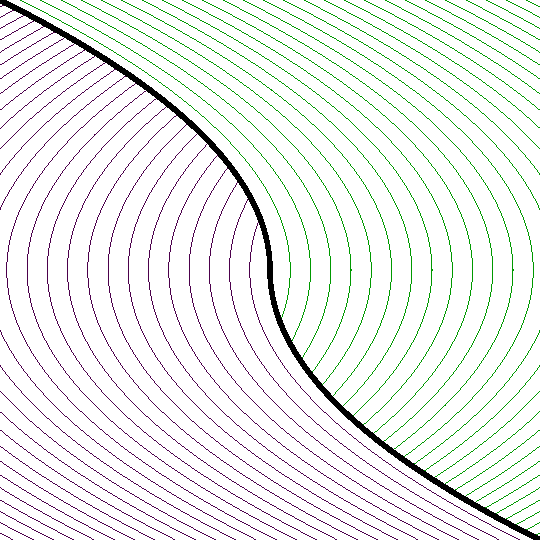
\includegraphics{figures/optimalswitching.pdf}}
\end{center}

\setcounter{tocdepth}{1}

\vspace{20.0pt}

\tableofcontents


\newpage


\section*{Part 1. Hamiltonian and Lagrangian mechanics}
\addtocounter{section}{1}
\setcounter{subsection}{0}

\subsection{Introduction}

Newton made the famous discovery that the motion of physical bodies can be described by a second-order differential equation
\eqst { \mathbf{F} = m \mathbf{a}, }
where $\mathbf{a}$ is the acceleration (the second derivative of the position of the body), $m$ is the mass, and $\mathbf{F}$ is the force, which has to be specified in order for the motion to be determined (for example, Newton's law of gravity gives a formula for the force $\mathbf{F}$ arising out of the gravitational influence of celestial bodies). The quantities $\mathbf{F}$ and $\mathbf{a}$ are vectors, but in simple problems where the motion is along only one axis can be taken as scalars.

In the 18th and 19th centuries it was realized that Newton's equations can be reformulated in two surprising ways. The new formulations, known as \emph{Lagrangian} and \emph{Hamiltonian} mechanics, make it easier to analyze the behavior of certain mechanical systems, and also highlight important theoretical aspects of the behavior of such systems which are not immediately apparent from the original Newtonian formulation. They also gave rise to an entirely new and highly useful branch of mathematics called the \emph{calculus of variations}---a kind of ``calculus on steroids'' (see Section~\ref{sec:variational-calculus}).

Our goal in this chapter is to give an introduction to this deep and beautiful part of the theory of differential equations. For simplicity, we restrict the discussion mostly to systems with one degree of freedom, and comment only briefly on higher-dimensional generalizations.

\subsection{Hamiltonian systems}

Recall that the general form of a planar differential equation (i.e., a system of two first-order ODEs) is
\eq{ \label{eq:genericsystem}
\dot{p} &= F(p,q,t), \\
\dot{q} &= G(p,q,t),
}
where, in keeping with a tradition in the theory of ODEs, $\dot{f}$ denotes the derivative of a quantity $f$ with respect to the time variable $t$.
The system is called a \emph{Hamiltonian system} if there is a function 
$$H=H(p,q,t)$$ 
(called the \emph{Hamiltonian} associated with the system) such that the functions $F$ and $G$ satisfy $$F(p,q,t) = -\frac{\partial H}{\partial q}, \quad G(p,q,t) = \frac{\partial H}{\partial p}.$$
In this case the system has the form
\eq{ \label{eq:hamiltoniansystem}
\dot{p} &= -\frac{\partial H}{\partial q}, \\
\dot{q} &= \ \ \frac{\partial H}{\partial p}.
}
The variable $p$ is sometimes called a \emph{generalized coordinate}, and the variable $q$ is called the \emph{generalized momentum} associated to $p$.

When can we say that a given system \eqref{eq:genericsystem} is Hamiltonian? Assuming that $F$ and $G$ are continuously differentiable, it is not difficult to see that a necessary condition is that
\eq{ \label{eq:hamiltonian-sufficient}
\frac{\partial F}{\partial p} = -\frac{\partial G}{\partial q},
}
(or $\frac{\partial F}{\partial p} +\frac{\partial G}{\partial q}=0$) since both sides of the equation are equal to $-\frac{\partial^2 H}{\partial p \partial q}$. Equivalently, this condition can be written as
$$ \divr \mathbf{V} = 0, $$
where $\mathbf{V}$ denotes the planar vector field $\mathbf{V}= (F,G)$ (we interpret the first coordinate of $\mathbf{V}$ as the ``$p$-coordinate'' and the second coordinate as the ``$q$-coordinate''), and $\divr \mathbf{V}$ denotes the divergence of $\mathbf{V}$. In physics, a vector field with this property is called \emph{divergence-free} or \emph{solenoidal}. Yet another way to write \eqref{eq:hamiltonian-sufficient} is
\eqst{
\curl \mathbf{W} = 0, 
}
where $\mathbf{W}$ is the vector field $\mathbf{W}=(G,-F)$, and $\curl$ is the (2-dimensional version of the) curl operator, defined by $\curl(A,B) = \frac{\partial A}{\partial q}-\frac{\partial B}{\partial p}$. A vector field with this property is called \emph{curl-free} or \emph{irrotational}.

\begin{lem} \label{lem:hamiltonian-div}
If the equation \eqref{eq:genericsystem} is defined on a simply connected domain, the condition \eqref{eq:hamiltonian-sufficient} is both necessary and sufficient for the system to be Hamiltonian.
\end{lem}

\begin{proof} This is a slight reformulation of a familiar fact from vector calculus, that says that in a simply connected domain, a vector field $\mathbf{W}=(A,B)$ is curl-free if and only if it is \emph{conservative}. A conservative vector field is one for which the line integral of the field between two points is independent of the contour connecting them, or equivalently, such that the line integral on any \emph{closed} contour vanishes. Such a vector field can always be represented as $\mathbf{W} = \grad H$ (the gradient of $H$) for some scalar function $H$; one simply defines $H(p,q)$ as the line integral (which for a conservative field is independent of the path of integration)
$$ H(p,q) = \int_{(p_0,q_0)}^{(p,q)} \mathbf{W}\cdot \mathbf{ds} = \int_{(p_0,q_0)}^{(p,q)} A\,dp + B\,dq
$$
between some fixed but arbitrary initial point $(p_0,q_0)$ and the point $(p,q)$. The fact that $\mathbf{W}=\grad H$ is immediate from the fundamental theorem of calculus. In our case, $\mathbf{W}=(G,-F)$ so the equation $\mathbf{W}=\grad H$ gives exactly the pair of equations $F=-\frac{\partial H}{\partial q}$, $G=\frac{\partial H}{\partial p}$, with $H$ serving as the desired Hamiltonian.
\end{proof}


\subsection{The Euler-Lagrange equation} Given a function of three variables $L=L(\dot{q},q,t)$, the differential equation
\eq{ \label{eq:euler-lagrange}
\frac{d}{dt}\left( \frac{\partial L}{\partial \dot{q}} \right) = \frac{\partial L}{\partial q}
}
is called the \emph{Euler-Lagrange equation}. Note that the notation here may be slightly confusing: for the purpose of computing $L(\dot{q},q,t)$ and finding $\frac{\partial L}{\partial \dot{q}}$, one must think of $\dot{q}$ as an independent variable that has no connection to $q$. But once $\frac{\partial L}{\partial \dot{q}}$ is evaluated, to apply the time-derivative $\frac{d}{dt}$, one should think of $\dot{q}$ as the time-derivative of $q$. This leads to a second-order ordinary differential equation for the quantity $q$. The function $L$ is called the \emph{Lagrangian}.

\subsection{Equivalence of the Lagrange and Hamilton formalisms}

We now wish to show that the Euler-Lagrange equation is equivalent to the idea of a Hamiltonian system. Start with the equation \eqref{eq:euler-lagrange}. Denote $p=\frac{\partial L}{\partial \dot{q}}$. The Hamiltonian will be defined by
\eq{ \label{eq:hamilton-lagrange}
H(p,q,t) = p\dot{q} - L(\dot{q}, q, t),
}
where $\dot{q}$ is again interpreted as a symbol representing an independent variable, which is extracted from $p, q, t$ by inverting the relation $p=\frac{\partial L}{\partial \dot{q}}$ (i.e., this relation defines a transformation from the system of variables $\dot{q},q,t$ to the system $p,q,t$). Then, using the chain rule we can compute
\eqst{
\pder{H}{p} &= \dot{q} + p \pder{\dot{q}}{p} - \pder{L}{\dot{q}} \pder{\dot{q}}{p} = 
\dot{q} + p \pder{\dot{q}}{p} - p \pder{\dot{q}}{p} = \dot{q}, \\
\pder{H}{q} &= p \pder{\dot{q}}{q} - \pder{L}{\dot{q}}\pder{\dot{q}}{q}-\pder{L}{q} = -\pder{L}{q} =
- \der{}{t} \left( \pder{L}{\dot{q}}\right) = -\der{p}{t} = -\dot{p},
}
which shows that we indeed get the Hamiltonian system \eqref{eq:hamiltoniansystem}.

Going in the other direction, if we start with a Hamiltonian system, we can construct a Lagrangian by setting
\eq{ \label{eq:lagrange-hamilton}
L(\dot{q}, q, t) = p\dot{q} - H(p,q,t),
}
where in this definition $p=p(q,\dot{q},t)$ is interpreted as a function of the independent variables $q, \dot{q}, t$, defined by the implicit equation $\dot{q} = \pder{H}{p}$. Again computing using the chain rule and the Hamiltonian equations \eqref{eq:hamiltoniansystem}, we now have that
\eqst{
\pder{L}{\dot{q}} &= p + \dot{q} \pder{p}{\dot{q}} - \pder{H}{p} \pder{p}{\dot{q}} = p, \\
\pder{L}{q} &= \dot{q}\pder{p}{q}-\pder{H}{p}\pder{p}{q}-\pder{H}{q}=-\pder{H}{q}=\dot{p} = \der{}{t} 
\left( \pder{L}{\dot{q}} \right),
}
so we have recovered the Euler-Lagrange equation \eqref{eq:euler-lagrange}.

\beginexercise{Legendre transform} The connection between the Hamiltonian and Lagrangian is that each is obtained from the other via a transformation called the \emph{Legendre transform}. Here is a simplified version of the definition of this transform: given a strictly convex smooth function $f(x)$ defined on some interval $[x_0,x_1]$ (i.e., $f''>0$), its Legendre transform is a function $g(p)$ defined on the interval $[p_0,p_1]$, where $p_i=f'(x_i)$. To compute $g(p)$, we first find the point $x$ such that $p=f'(x)$, and then set
\eqst{
g(p) = px - f(x).
}
\begin{enumerate}
\item Prove that $g$ is also strictly convex.
\item Prove that the Legendre transform is its own inverse: i.e., $f(x)$ is the Legendre transform of $g(p)$.
\item Compute the Legendre transforms of the following functions: (i) $f(x)=x^{\alpha}, \alpha>1$; (ii) $f(x)=e^x$; (iii) $f(x)=\cosh x$.
\end{enumerate}



\subsection{Lagrangian formulation of Newtonian mechanics} Assume a particle of mass $m$ is constrained to move in one dimension under the influence of a force $F=F(q,t)$, where $q$ is the position coordinate. The equation of motion is
\eq{ \label{eq:newtonmotion}
\ddot{q} = \frac{F}{m} = -\pder{U}{q},
}
where $U=U(q,t)$ is the potential energy per unit mass associated with the force $F$ at time $t$, defined by $U(q)=-\frac{1}{m}\int_{q_0}^ q F(u)\,du$.
Define a Lagrangian $L=L(\dot{q},q,t)$ by
$$ 
L(\dot{q},q,t) = \tfrac12 \dot{q}^2 - U(q,t)
$$
(the kinetic energy of the particle \emph{minus} the potential energy, divided by its mass). Now let us write the Euler-Lagrange equation for this Lagrangian. The relation $p=\pder{L}{q} = \dot{q}$ means that $p$ is simply equal to the velocity of the particle, and \eqref{eq:euler-lagrange} becomes
$$ \ddot{q} = \dot{p} = \der{}{t} \left( \pder{L}{\dot{q}} \right) = \pder{L}{q} = -\pder{U}{q}, $$
which is the same as \eqref{eq:newtonmotion}. The strange-looking Lagrangian formalism has reproduced Newton's equation of motion! Also note that the Hamiltonian associated with the system, related to the Lagrangian by equations \eqref{eq:hamilton-lagrange} and \eqref{eq:lagrange-hamilton}, is
\eqst{
H = p \dot{q} - L = \dot{q}^2 - \left( \tfrac12 \dot{q}^2 - U(q,t) \right)
= \tfrac12 \dot{q}^2 + U(q,t), 
}
i.e., the Hamiltonian is the kinetic energy \emph{plus} the potential energy, or the total energy of the particle, divided by the mass.

Let us now see whether this phenomenon can be generalized. Assume that the particle is now moving in \emph{three} dimensions, so its position $\mathbf{x}(t)$ as a function of time is a vector, which varies under the influence of an external force field, which we take to be conservative. However, since we prefer to keep working with planar ODEs for the time being, assume that the motion of the particle is nonetheless constrained to lie on some one-dimensional curve $\Gamma=\Gamma_t$ (which could itself be moving in space, so depends on $t$). For example, the physical interpretation can be of a bead sliding without friction along a curved wire, which may be moving in space. In this case, the equation of motion can be written in the form
\eq{ \label{eq:curve-forces}
\ddot{\mathbf{x}} - \frac{1}{m}\mathbf{F} = \ddot{\mathbf{x}} + \grad U = \frac{1}{m} \mathbf{G}(\mathbf{x},t),
}
where $\mathbf{F}(\mathbf{x},t)$ denotes the external force field, associated with the potential energy $U(\mathbf{x},t)$, and where a second force function $\mathbf{G}(\mathbf{x},t)$ is a \emph{constraint force} acting in a direction normal to the curve $\Gamma_t$. The role of the constraint force is to make sure that the particle's trajectory remains constrained to the curve.

Now, since the particle is constrained to a curve, we should be able to describe its position at any instant using a single real number. That means introducing a new (scalar) quantity $q$, such that $\mathbf{x}$ can be described in terms of a functional relation with $q$:
\eqst { \mathbf{x} = \mathbf{x}(q,t). }
The idea is that $q$ is a parameter measuring position along the curve (in a way that may depend on $t$) in some way. For example, $q$ may measure arc length along the curve as measured from some known reference point $\mathbf{x_0}(t)$ on the curve. The details of the definition of $q$ depend on the specific problem (there are many possible choices of $q$ for a given situation) and are not important for the present analysis.

Let us now show that the equation of motion can be represented using the Lagrangian formalism as applied to the new coordinate $q$. Begin by observing that we have the relation
\eqst{ \mathbf{G}\cdot \pder{\mathbf{x}}{q} = 0, }
since $\mathbf{G}$ acts normally to the curve and $\pder{\mathbf{x}}{q}$ is tangential to it. Then taking the scalar product of both sides of \eqref{eq:curve-forces} with $\pder{\mathbf{x}}{q}$ gives
\eqst{ 
\ddot{\mathbf{x}} \cdot \pder{\mathbf{x}}{q} + (\grad U) \cdot \pder{\mathbf{x}}{q} = 0,
}
or 
\eq{ \label{eq:curveeq1}
\ddot{\mathbf{x}} \cdot \pder{\mathbf{x}}{q} + \pder{U}{q} = 0,
}
where we now interpret $U=U(\mathbf{x},t)$ as a function $U(q,t)$ of $q$ and $t$. Now define the Lagrangian $L$ by again taking the difference of the kinetic and potential energies, namely
\eqst{
L = \tfrac12 |\dot{\mathbf{x}}|^2 - U
= \tfrac12 \left| \pder{\mathbf{x}}{q} \dot{q} + \pder{\mathbf{x}}{t} \right|^2 - U,
}
which can be interpreted as a function of $q$, $\dot{q}$ and $t$. Note that 
the velocity $\dot{\mathbf{x}}=\pder{\mathbf{x}}{q} \dot{q} + \pder{\mathbf{x}}{t}$, also considered as a function of $q, \dot{q}$ and $t$, satisfies
$$ \pder{\dot{\mathbf{x}}}{\dot{q}} = \pder{\mathbf{x}}{q}. $$
Taking partial derivatives of $L$ with respect to $q$ and $\dot{q}$, we get
\eq{ \label{eq:curveeq2}
\pder{L}{\dot{q}} &= 
\tfrac12 \pder{}{\dot{q}} \left( \dot{\mathbf{x}}\cdot \dot{\mathbf{x}} \right)
=
\dot{\mathbf{x}} \cdot \pder{\mathbf{x}}{q}, \\
\pder{L}{q} &= 
\tfrac12 \pder{}{q} \left( \dot{\mathbf{x}}\cdot \dot{\mathbf{x}} \right) - \pder{U}{q}
=
\dot{\mathbf{x}}\cdot \pder{\dot{\mathbf{x}}}{q}-\pder{U}{q}.
}
Also, note that
\eq{ \label{eq:curveeq3}
\der{}{t}\left(\pder{\mathbf{x}}{q}\right) = \pder{\hspace{1pt}^2 \mathbf{x}}{q^2}\dot{q}
+ \pder{\hspace{1pt}^2 \mathbf{x}}{q\partial t} = \pder{}{q}
\left( \pder{\mathbf{x}}{q}\dot{q}+\pder{\mathbf{x}}{t}
\right) = \pder{\mathbf{\dot{x}}}{q}
}
Combining the results \eqref{eq:curveeq1}, \eqref{eq:curveeq2} and \eqref{eq:curveeq3}, we get finally that
\eqst{
\der{}{t}\left(\pder{L}{\dot{q}}\right)
&=
\ddot{\mathbf{x}} \cdot \pder{\mathbf{x}}{q}
+ \dot{\mathbf{x}}\cdot \der{}{t}\left( \pder{\mathbf{x}}{q}\right)
%\\ &
=
\ddot{\mathbf{x}} \cdot \pder{\mathbf{x}}{q}
+ \dot{\mathbf{x}} \cdot \pder{\dot{\mathbf{x}}}{q}
\\ &= 
\ddot{\mathbf{x}} \cdot \pder{\mathbf{x}}{q}
+ \pder{}{q}\left(\tfrac12|\dot{\mathbf{x}}|^2\right)
= -\pder{U}{q}+\pder{}{q}(L+U)
\\ &= \pder{L}{q}.
}
Thus, the equation of motion becomes the Euler-Lagrange equation for the Lagrangian $L$ when the motion is parametrized using the scalar coordinate $q$.

It is interesting to find also the Hamiltonian associated with the system. Is it equal to the total energy per unit mass? The energy per unit mass is
\eqst{ E = K + U, }
where $U$ is the potential energy and $K = \tfrac12|\dot{x}|^2$ is the kinetic energy, which can be written more explicitly as
\eqst{
K = \tfrac12 \left|\pder{\mathbf{x}}{q}\right|^2 \dot{q}^2 + \left(\pder{\mathbf{x}}{q}\cdot\pder{\mathbf{x}}{t}\right)
\dot{q} + \tfrac12\left|\pder{\mathbf{x}}{t}\right|^2,
}
(a quadratic polynomial in $\dot{q}$). The generalized momentum coordinate $p$ is in this case given by
\eqst{
p = \pder{L}{\dot{q}} = 
\left|\pder{\mathbf{x}}{q}\right|^2 \dot{q} + \pder{\mathbf{x}}{q}\cdot\pder{\mathbf{x}}{t}.
}
Note that it is in one-to-one correspondence with $\dot{q}$, as should happen. By \eqref{eq:hamilton-lagrange}, we get the Hamiltonian as
\eqst{
H &= 
\left|\pder{\mathbf{x}}{q}\right|^2 \dot{q}^2 + \left(\pder{\mathbf{x}}{q}\cdot\pder{\mathbf{x}}{t}\right)\dot{q} - L
\\ &=
\left|\pder{\mathbf{x}}{q}\right|^2 \dot{q}^2 + \left(\pder{\mathbf{x}}{q}\cdot\pder{\mathbf{x}}{t}\right)\dot{q} - (K-U)
\\ &= E - \left(\pder{\mathbf{x}}{q}\cdot\pder{\mathbf{x}}{t}\right)\dot{q} -
\tfrac12\left|\pder{\mathbf{x}}{t}\right|^2.
}
In particular, if $\mathbf{x}$ does not have an explicit dependence on $t$ (which corresponds to a situation in which $\mathbf{x}=\mathbf{x}(q)$, i.e., the constraint curve is stationary), then $\pder{\mathbf{x}}{t}=0$, and in this case $H=E$. However, in the general case the Hamiltonian differs from the energy of the system.

%\subsection{Examples} We illustrate the above discussion with a few examples.

%\subsubsection*{Example 1. the harmonic oscillator}

\beginexample{The harmonic oscillator}
The one-dimensional harmonic oscillator corresponds to the motion of a particle in a parabolic potential well, $U(q)=\tfrac12 k q^2$, where $k>0$, or equivalently, motion under a linear restoring force $F(q)=-m k q$ (e.g., an oscillating weight attached to an idealized elastic spring satisfiying Hooke's law). In this case we have
\eqst{ 
L &= \tfrac12 \dot{q}^2 - \tfrac12 kq^2, \\ 
H &= \tfrac12 \dot{q}^2 + \tfrac12 kq^2, \\
p &= \pder{L}{\dot{q}} = \dot{q},
}
and the equation of motion $\der{}{t}\left(\pder{L}{\dot{q}}\right)=\pder{L}{q}$ is
\eqst{
\ddot{q} = -kq.
}
Its general solution has the form
\eqst{ q = A\cos(\omega t) + B \sin(\omega t), }
where $\omega= \sqrt{k}$.

%\subsubsection*{Example 2. The simple pendulum}
\beginexample{The simple pendulum}
Next, consider the simple pendulum, which consists of a point mass $m$ attached to the end of a rigid rod of length $\ell$ and negligible mass, whose other end is fixed to a point and is free to rotate in one vertical plane. This simple mechanical system also exhibits oscillatory behavior, but its behavior is much richer and more complex due to the nonlinearity of the underlying equation of motion. Let us use the Lagrangian formalism to derive the equation of motion. This is an example of the more generalized scenario of motion constrained to a curve (in this case a circle). The natural choice for the generalized coordinate $q$ is the angle $q=\theta$ between the two vectors pointing from the fixed end of the rod in the down direction and towards the pendulum, respectively. In this case, we can write
\eqst{
\mathbf{x} &= (\ell\sin q, 0, -\ell \cos q), \\
K &= \textrm{Kinetic energy per unit mass} = \tfrac12|\dot{\mathbf{x}}|^2 = \tfrac12 \ell^2 \dot{q}^2, \\
U &= \textrm{Potential energy per unit mass} = -g\ell\cos q, \\
L &= K-U = \tfrac12 \ell^2 \dot{q}^2 + g \ell \cos q, \\
p &= \pder{L}{\dot{q}} = \ell^2 \dot{q}, \\
H &= E = K+U = \tfrac12 \ell^2 \dot{q}^2 - g \ell\cos q
= \frac{p^2}{2\ell^2} - g\ell\cos q.
}
The equation of motion becomes $\ell^2 \ddot{q}=\dot{p} = \pder{L}{q}=-g\ell \sin q$, or
\eqst{
\ddot{q} = -\frac{g}{\ell} \sin q.
}
This is often written in the form
\eq{ \label{eq:pendulumeq}
\ddot{q} + \omega^2 \sin q = 0,
}
where $\omega^2 = \frac{g}{\ell}$. In Hamiltonian form, the equations of motion will be
\eqst{ \dot{p}&= -g\ell \sin q, \\ \dot{q}&=\frac{p}{\ell^2}. }

%\subsubsection*{Example 3. A rotating pendulum} 
\beginexample{A rotating pendulum}
Let us complicate matters by assuming that the pendulum is rotating around the vertical axis (the $z$-axis, in our coordinate system) with a fixed angular velocity $\omega$. In terms of the coordinate $q$, which still measures the angle subtended between the vector pointing from the origin to the particle and the vertical, the particle's position will now be
\eqst{
\mathbf{x} = (\ell \sin q \cos(\omega t), \ell \sin q \sin(\omega t), -\ell\cos(\omega t)). 
}
The kinetic and potential energies per unit mass, and from them the Lagrangian and Hamiltonian, and the generalized momentum coordinate $p$, can now be found to be
\eqst{
K &= \tfrac12|\dot{x}|^2 = \tfrac12 \ell^2(\dot{q}^2 + \omega^2 \sin^2 q), \\
U &= -g\ell \cos q, \\
L &= \tfrac12\ell^2(\dot{q}^2+\omega^2\sin^2 q)+g\ell\cos q, \\
p &= \ell^2 \dot{q}, \\
H &= \frac{p^2}{2\ell^2}-g\ell\cos q-\tfrac12 \omega^2 \ell^2 \sin^2 q.
}
The Euler-Lagrange equation of motion is
\eqst{
\ddot{q} + \Omega^2 \sin q - \omega^2 \sin q \cos q = 0,
}
where $\Omega^2 = \frac{g}{\ell}$. The system in Hamiltonian form is
\eqst{
\dot{p} &= -g\ell \sin q + \omega^2 \ell^2 \sin q \cos q, \\
\dot{q} &= \frac{p}{\ell^2}.
}

\subsection{An autonomous Hamiltonian is conserved} In the last example above, it is important to note that although the system in its original form depends on time due to the motion of the constraint curve, the Hamiltonian, Lagrangian and the associated equations are \emph{autonomous}, i.e., do not depend on time. This is an illustration of the type of simplification that can be achieved using the Lagrangian and Hamiltonian formulations. Furthermore, the fact that the Hamiltonian is autonomous has an important consequence, given by the following lemma.

\begin{lem} \label{lem:hamiltonian-conserved}
If the Hamiltonian is autonomous, then $H$ is an integral (i.e., an invariant or conserved quantity) of Hamilton's equations.
\end{lem}

\begin{proof} The assumption means that $\pder{H}{t} = 0$. By the chain rule, it follows that
\eqst{
\der{H}{t} &= \pder{H}{p} \dot{p}+\pder{H}{q} \dot{q} + \pder{H}{t}
\\ &= \pder{H}{p}\left(-\pder{H}{q}\right)+\pder{H}{q}\left(\pder{H}{p}\right)+\pder{H}{t}
= \pder{H}{t} = 0.
}
\end{proof}

In the first two examples of the harmonic oscillator and the simple pendulum, the Hamiltonian was equal to the system's energy, so Lemma~\ref{lem:hamiltonian-conserved} corresponds to the conservation of energy. In the example of the rotating pendulum, the Hamiltonian is \emph{not} equal to the energy of the system, yet it is conserved. Can you think of a physical meaning to assign to this conserved quantity?

\subsection{Systems with many degrees of freedom}

In the above discussion, we focused on a system with only one degree of freedom. In this case the equations of motion consisted of a single second order differential equation (the Euler-Lagrange equation), or in the equivalent Hamiltonian form, a planar system of first-order equations. We can describe the behavior of systems having more degrees of freedom, involving for example many particles or an unconstrained particle moving in three dimensions, using a multivariate form of the Euler-Lagrange and Hamilton equations. We describe these more general formulations of the laws of mechanics briefly, although we will not develop this general theory here.

Let the system be described by $n$ generalized coordinates $q_1, \ldots, q_n$. The Lagrangian will be a function of the coordinates and their time derivatives (generalized velocities):
\eqst{ L = L(q_1,\ldots,q_n,\dot{q}_1,\ldots,\dot{q}_n, t) }
As before, the Lagrangian will be defined as the kinetic energy minus the potential energy of the system. The equations of motion will be given as a system of Euler-Lagrange second-order equations, one for each coordinate:
\eqst{
\frac{d}{dt}\left( \frac{\partial L}{\partial \dot{q}_j} \right) = \frac{\partial L}{\partial q_j} \ \ \quad (j=1,\ldots,n).
}
To write the Hamiltonian formulation of the system, first we define generalized momentum coordinates $p_1,\ldots,p_n$. They are given analogously to the one-dimensional case by
\eqst{ 
p_j = \pder{L}{\dot{q}_j} \ \ \quad (j=1,\ldots,n).
}
The Hamiltonian system is written as a system of $2n$ first-order ODEs:
\eqst{ \begin{array}{rl} \displaystyle
\dot{p}_j &= \displaystyle-\frac{\partial H}{\partial q_j}, \raisebox{-20pt}{\ } \\
\displaystyle \dot{q}_j &= \displaystyle \ \ \frac{\partial H}{\partial p_j},
\end{array} \qquad (j=1,\ldots,n),
}
where $H=H(p_1,\ldots,p_n,q_1,\ldots,q_n, t)$ is the Hamiltonian, which (like the Lagrangian) is still a scalar function.
This is sometimes written as the pair of vector equations
\eqst{
\dot{\mathbf{p}} &= -\frac{\partial H}{\partial \mathbf{q}}, \\
\dot{\mathbf{q}} &= \ \ \frac{\partial H}{\partial \mathbf{p}},
}
where we denote $\mathbf{p}=(p_1,\ldots,p_n)$, $\mathbf{q}=(q_1,\ldots,q_n)$.

As in the case of one-dimensional systems, it can be shown that (under some mild assumptions) the Hamiltonian and Lagrangian formulations are equivalent, and that they correctly describe the laws of motion for a Newtonian mechanical system if the Lagrangian is defined as the kinetic energy minus the potential energy. The relationship between the Lagrangian and Hamiltonian is given by
\eqst{
H = \sum_{j=1}^n \dot{q}_j p_j - L.
}

%\subsubsection*{Example 4. A pendulum with a sliding support} 
\beginexample{A pendulum with a cart}
An important example that we will discuss later from the point of view of control theory is that of a simple pendulum whose point of support is allowed to slide without friction along a horizontal axis (e.g., you can imagine the pendulum hanging on a cart with wheels rolling on a track of some sort). We assume the sliding support has mass $M$. This system has two degrees of freedom: the angle $q_1 = \theta$ between the pendulum and the vertical line extending down from the point of support, and the distance $q_2 = s$ (measured in the positive $x$ direction) between the point of support and some fixed origin. To derive the equations of motion, we write the kinetic and potential energies:
\eqst{
K &= \tfrac12 M \dot{s}^2 + \tfrac12 m \left[ \left(\dot{s}+\ell \dot{\theta} \cos \theta \right)^2 + \left(\ell \dot{\theta} \sin \theta \right)^2 \right], \\
U &= -mg \ell \cos \theta.
}
The Lagrangian $L=K-U$ is then given by
\eqst{
L &=
\tfrac12 M \dot{s}^2 + \tfrac12 m \left[ \left(\dot{s}+\ell \dot{\theta} \cos \theta \right)^2 + \left(\ell \dot{\theta} \sin \theta \right)^2 \right] + mg \ell \cos \theta \\
&= \tfrac12(M+m)\dot{s}^2 + m\ell \dot{s} \dot{\theta} \cos \theta + \tfrac12 m \ell^2 \dot{\theta}^2 + mg\ell \cos\theta.
}
Therefore the equations of motion $\der{}{t}\left(\pder{L}{\dot{s}}\right)=\pder{L}{s}$,
$\der{}{t}\left(\pder{L}{\dot{\theta}}\right)=\pder{L}{\theta}$ become
\eqst{
\der{}{t}\left[ (M+m)\dot{s} + m\ell\dot{\theta}\cos \theta \right] &= 0, \\
\der{}{t}\left[m(\ell \dot{s}  \cos\theta + \ell^2 \dot{\theta})\right] &= -m(\ell\dot{s} \dot{\theta} + g\ell)\sin \theta, 
}
or, written more explicitly,
\eqst{
(M+m)\ddot{s} + m\ell \ddot{\theta} \cos \theta -m\ell \dot{\theta}^2 \sin\theta &= 0, \\
\ddot{\theta} + \frac{1}{\ell}\ddot{x} \cos\theta + \frac{g}{\ell}  \sin\theta &= 0.
}

\beginexample{Double pendulum} The double pendulum consists of a mass $M$ hanging at the end of a rigid rod of negligible mass whose other end is attached to a fixed point of support, and another equal (for simplicity) mass hanging from another rigid rod, also of negligible mass attached to the free end of the first rod. Denote by $L_1$ and $L_2$ the respective lengths of the two rods. If we denote by $\theta_1, \theta_2$ the angles each of the rods forms with the vertical, a short computation gives the Lagrangian of the system:
\eq{ \label{eq:lagrangian-doublepend}
L &= K-U = 
L_1 \dot{\theta}_1^2 + \tfrac12 L_2 \dot{\theta}_2^2 + L_1 L_2 \cos(\theta_1-\theta_2)
\\ & \qquad\qquad \qquad +2gL_1 \cos \theta_1 + gL_2 \cos \theta_2.
}
It follows that the generalized momenta are given by
\eqst{
p_1 &= \pder{L}{\dot{\theta}_1} = \tfrac12 L_1^2 \dot{\theta}_1 - 2 L_1 L_2 \sin(\theta_1-\theta_2), \\
p_2 &= \pder{L}{\dot{\theta}_2} = \tfrac12 L_2^2 \dot{\theta}_2 + 2 L_1 L_2 \sin(\theta_1 - \theta_2),
}
and from this we get the equations of motion for the system:
\eqst{
%\dot{p}_1 &=
 \tfrac12 L_1^2 \ddot{\theta}_1 - 2 L_1 L_2 \cos(\theta_1-\theta_2)\dot{\theta}_1 &= 
- L_1 L_2 \sin(\theta_1-\theta_2) + g L_1 \sin\theta_1, \\
%\dot{p}_2 &= 
\tfrac12 L_2^2 \ddot{\theta}_2 - 2 L_1 L_2 \cos(\theta_1-\theta_2)\dot{\theta}_2 &= 
L_1 L_2 \sin(\theta_1-\theta_2) + gL_2 \sin\theta_2. 
}
This system of two nonlinear coupled second-order ODEs is in practice impossible to solve analytically, and for certain values of the energy is known to exhibit chaotic behavior which is difficult to understand in any reasonable sense; see Figure~\ref{fig:doublependulum-flips}. (Nonetheless, later in the course we will learn about some interesting things that can still be said about such systems.)

\begin{figure}
\begin{center}
\scalebox{0.25}{
\includegraphics{figures/doublependulum-flips.png}}
\caption{A color-coded map of the time required for the double pendulum to flip over as a function of its initial conditions reveals a chaotic structure. (Source: Wikipedia) \label{fig:doublependulum-flips}}
\end{center}
\end{figure}


%Note that the Lagrangian $L$ in \eqref{eq:lagrangian-doublepend} is symmetric under the  exchange of system parameters: $(L_1, \theta_1, \dot{\theta}_1) \leftrightarrow (L_2, \theta_2, \dot{\theta}_2)$. It follows that the equations of motion have the same symmetry; physically, this means that the pendulum will behave the same if we exchange the order of the two rods. Can you think of an intuitive explanation for this phenomenon? (For example, try imagining a system with one very short rod and one long, arranged in the two different possible orders, and comparing their evolutions.)


%\beginexample{One body problem in a central gravitational field}
%The (vector) equation of motion for a particle of mass $m$ moving under the influence of a conservative force field $\mathbf{F}=-m \grad U$ (where $U$ is the potential energy per unit of mass) is
%\eqst{
%\ddot{\mathbf{x}} = - \grad U.
%}
%Assume that $U$ is a \emph{central} potential, i.e., depends only on the distance $|\mathbf{x}|$ of $\mathbf{x}$ from the origin. That is, we can write $U = U(|\mathbf{x}|)$. In this case, we will show that the system of three equations describing the motion of the particle can be reduced to a single equation.
%***finish this***
%
%\beginexample{Two body problem}
%*** add this ***
%
%\beginexample{Spinning top}
%*** add this ***

\beginexercise{The Lorentz force} From the study of electricity and magnetism, it is known that the motion of a charged particle with mass $m$ and electric charge $q$ is described by the equation $\mathbf{F}=m \ddot{\mathbf{x}}$, where $\mathbf{x}$ is the (vector) position of the particle and $\mathbf{F}$ is the \emph{Lorentz force}, given by
$$ \mathbf{F} = q\left(\mathbf{E} + \dot{\mathbf{x}}\times \mathbf{B}\right). $$
The vector field $\mathbf{E}=\mathbf{E}(x,y,z,t)$ is the \emph{electric field}, and the vector field $\mathbf{B}=\mathbf{B}(x,y,z,t)$ is the \emph{magnetic field}. Using Maxwell's equations one can show that there exist functions $\phi=\phi(x,y,z,t)$ and $\mathbf{A}=\mathbf{A}(x,y,z,t)$ such that
\eqst{
\mathbf{E} &= - \grad \phi - \pder{\mathbf{A}}{t}, \\
\mathbf{B} &= \curl \mathbf{A}.
}
The (scalar) function $\phi$ is called the \emph{electric potential}, and the vector $\mathbf{A}$ is called the \emph{magnetic potential}, or \emph{vector potential}. Note that $\mathbf{E}$ behaves exactly like a conventional force field, causing the particle an acceleration in the direction of $\mathbf{E}$ that is equal to the field magnitude multiplied by the (constant) scalar $q/m$, whereas the influence of the magnetic field $\mathbf{B}$ is of a more exotic nature, causing an acceleration that depends on the particle's \emph{velocity} in a direction perpendicular to its direction of motion.

\smallskip \noindent Show that motion under the Lorentz force is equivalent to the Euler-Lagrange equation $ \der{}{t}\left(\pder{L}{\dot{\mathbf{x}}}\right)=\pder{L}{\mathbf{x}}$, where the Lagrangian is given by
$$ L(\dot{\mathbf{x}},\mathbf{x},t) = \tfrac12 m |\dot{\mathbf{x}}|^2 - q \phi(\mathbf{x},t) +q \mathbf{A}(\mathbf{x},t)\cdot \dot{\mathbf{x}}. $$




\subsection{Rest points in autonomous Hamiltonian systems} Assume that the Hamiltonian is autonomous. The rest points of the system correspond to the stationary points of the Hamiltonian, i.e., points for which
\eqst{ \pder{H}{p} = 0, \quad \pder{H}{q} = 0. }
Let $(p_0,q_0)$ be a rest point of the system. We can analyze the stability properties of the rest point by linearizing. Setting
\eqst{ x = p-p_0, \quad y=q-q_0, }
the behavior of the system near $(p_0,q_0)$ can be described as
\eqst{
\dot{x} &= -bx-cy + O(x^2+y^2), \\ \dot{y}&= \ \ ax+by + O(x^2+y^2),
}
where
\eqst{
a = \frac{\partial^2 H}{\partial p^2} \raisebox{-5pt}{\Big|}_{(p_0,q_0)},\quad
b = \frac{\partial^2 H}{\partial p \partial q} \raisebox{-5pt}{\Big|}_{(p_0,q_0)}, \quad
c = \frac{\partial^2 H}{\partial q^2} \raisebox{-5pt}{\Big|}_{(p_0,q_0)}.
}

By the theory of stability analysis of planar ODEs, the stability type of the rest point can now be understood in terms of the behavior of the eigenvalues of the matrix
\eqst{ \left(\begin{array}{cc} -b&-c\\a&b\end{array}\right) }
(the Jacobian matrix of the vector field at the rest point). The eigenvalues are given by
\eqst{ \lambda^2 = b^2-ac. }
So we see that, when $b^2<ac,$ the eigenvalues are pure imaginary numbers, and recall that in that case the rest point is a center. On the other hand, when $b^2>ac$ the eigenvalues are the two real square roots $\pm \sqrt{b^2-ac}$. Since in that case we have one negative and one positive eigenvalue, the stability theory says that the rest point is a saddle point. (We assume that the Hessian matrix of second derivatives is non-degenerate, i.e., that $b^2\neq ac$, so that the usual criteria for stability apply.)
Liouville's theorem, which we will discuss in a later section, will give another, more geometric, explanation why rest points cannot be asymptotically stable or unstable.


\subsection{The principle of least action} For times $t_0<t_1$, define the \emph{action} $A(t_0,t_1)$ of a Lagrangian system from time $t_0$ to time $t_1$ as the integral of the Lagrangian:
\eqst{
A(t_0,t_1)=\textrm{action} = \int_{t_0}^{t_1} L(\dot{q}(t),q(t),t)\,dt.
}
The action is a function of an arbitrary curve $q(t)$.
The \emph{principle of least action} is the statement that if the system was in coordinate $q_0$ at time $t_0$ and in coordinate $q_1$ at time $t_1$, then its trajectory between time $t_0$ and time $t_1$ is that curve which minimizes the action $A(t_0,t_1)$, subject to the constraints $q(t_0)=q_0, q(t_1)=q_1$. This is a surprising statement, which we will see is \emph{almost} equivalent to the Euler-Lagrange equation---only almost, since, to get the equivalence, we will need to first modify the principle slightly to get the more precise version known as the \emph{principle of stationary action}.

The principle of least action can be thought of as a strange, \emph{non-causal} interpretation of the laws of mechanics. We are used to thinking of the laws of nature as manifesting themselves through interactions that are local in space and time: a particle's position $\mathbf{x}+d\mathbf{x}$ and velocity $\mathbf{v}+d\mathbf{v}$ at time $t+dt$, are related to its position $\mathbf{x}$ and velocity $\mathbf{v}$ at time $t$, as well as to external forces acting on the particle, which are also determined by ``local'' events in the vicinity of $\mathbf{x}$ at time $t$. This way of thinking can be thought of as the \emph{causal} interpretation, in which every effect produced at a given point in space and time is immediately preceded by, and can be directly attributable to, another event causing the effect. Mathematically, this means the laws of nature can be written as (ordinary or partial) differential equations. 

On the other hand, the principle of least action (and other similar principles that appear in physics, including in more fundamental areas of physics such as quantum mechanics, that we know represent a more correct view of our physical reality) can be thought of as saying that, in order to bring a physical system from state $A$ to state $B$ over a given period of time, Nature somehow tries all possible ways of doing it, and selects the one that minimizes the action. The entire trajectory appears to be chosen ``all at once,'' so that each part of it seems to depend on other parts which are far away in space and time. This rather unintuitive interpretation is nonetheless mathematically correct, and even at the physical level it has been suggested that there is some truth to it (the arguments for why this is so involve deep ideas from quantum mechanics that are beyond the scope of this course).

\subsection{The calculus of variations \label{sec:variational-calculus}} Let us consider the problem of minimizing the action in slightly greater generality. In many areas of mathematics we encounter expressions of the form
\eq{ \label{eq:functional}
\Phi(q) = \int_{t_0}^{t_1} L(\dot{q}(t),q(t),t)\,dt 
}
which take a (sufficiently smooth) function $q(t)$ defined on an interval $[t_0,t_1]$ and return a real number. The form of the integrand $L(\dot{q},q,t)$ depends on the problem, and may have nothing to do with Lagrangian mechanics (indeed, in many problems with a geometric flavor, $t$ represents a space variable instead of a time variable, and is therefore often denoted by $x$; in this case, we write $q'$ instead of $\dot{q}$ for the derivative of $q$). Usually the function $q$ is assumed to take specific values at the ends of the interval, i.e., $q(t_0)=q_0$ and $q(t_1)=q_1$.

Such a mapping $q\mapsto \Phi(q)$ is called a \emph{functional}---note that a functional is just like an ordinary function from calculus, except that it takes as its argument an entire function instead of only one or several real-valued arguments (that is why we call such functions \emph{functionals}, to avoid an obvious source of confusion). In many cases it is desirable to find which function $q$ results in the least and/or the greatest value $\Phi(q)$. Such a minimization or maximization problem is known as a \emph{variational problem} (the reason for the name is explained below), and the area of mathematics that deals with such problems is called the \emph{variational calculus}, or \emph{calculus of variations}. In more advanced variational problems the form of the functional \eqref{eq:functional} can be more general and depend for example on a vector-valued function $\mathbf{q}(t)$, or on higher-order derivatives of $q$, or on a function $q(x_1,\ldots,x_k)$ of several variables

Here are some examples of variational problems.
\begin{enumerate}
\item What is the shortest curve in the plane connecting two points? We all know it is a straight line, but how can we prove it? (And how do we find the answer to the same question on some complicated surface?)
\item What is the curve of given length in the plane bounding the largest area? (It is a circle---this fact, which is not trivial to prove, is known as the \emph{isoperimetric inequality}.)
\item What is the curve connecting a point $\mathbf{A}$ in the plane with another lower point $\mathbf{B}$ such that a ball rolling downhill without friction along the curve from $\mathbf{A}$ to $\mathbf{B}$ under the influence of gravity will reach $\mathbf{B}$ in the minimal possible time? This problem is known as the \emph{brachistochrone problem}, and stimulated the development of the calculus of variations in the 18th century.
\item What is the curve in the phase space of a Lagrangian system that minimizes the action?
\end{enumerate}

The basic idea involved in solving variational problems is as follows: if $q$ is an extremum (minimum or maximum) point of the functional $\Phi$, then it is also a \emph{local extremum}. That means that for any (sufficiently smooth) function $h:[t_0,t_1]\to \R$ satisfying $h(t_0)=h(t_1)=0$, the function
$$ \phi_{q,h}(s) = \Phi(q+s h)=\int_{t_0}^{t_1} L(\dot{q}(t)+sh'(t),q(t)+sh(t),t)\,dt  $$
(an ordinary function of a single real variable $s$) has a local extremum at $s=0$. From ordinary calculus, we know that the derivative of $\phi_{q,h}$ at $0$ must be $0$:
$$ \phi_{q,h}'(0) = 0. $$
To evaluate this derivative, differentiate under the integral sign and integrate by parts, to get
\eqst{
\phi_{q,h}'(0) 
&=
\int_{t_0}^{t_1} \der{}{s} \raisebox{-6pt}{\tiny \Big|s=0}  L(\dot{q}(t)+sh'(t),q(t)+sh(t),t)\,dt
\\
&= \int_{t_0}^{t_1} \left(\pder{L}{\dot{q}} h'(t) + \pder{L}{q} h(t) \right)\,dt
\\ &=
\int_{t_0}^{t_1} \left(-\der{}{t}\left(\pder{L}{\dot{q}}\right) + \pder{L}{q} \right)h(t)\,dt
+ \pder{L}{\dot{q}} h(t)\Big|_{t=t_0}^{t=t_1}
\\ &= \int_{t_0}^{t_1} \left(-\der{}{t}\left(\pder{L}{\dot{q}}\right) + \pder{L}{q} \right)h(t)\,dt
}
This brings us to an important definition. We denote
\eq{ \label{eq:first-variation}
\delta\Phi_q(h) = \int_{t_0}^{t_1} \left(-\der{}{t}\left(\pder{L}{\dot{q}}\right) + \pder{L}{q} \right)h(t)\,dt,
}
and call this quantity the \emph{variation of the functional} $\Phi$ at $q$, evaluated at $h$ (also sometimes called the \emph{first variation of $\Phi$}, since there is also a second variation, third variation etc., which we will not discuss; this is where the name \emph{calculus of variations} comes from). It is analogous to a directional derivative $\pder{f}{\mathbf{u}} = \nabla f \cdot \mathbf{u}$ of a function of several variables in calculus, in that it measures the instantaneous rate of change of $\Phi$ if we start from the ``point'' $q$ and head off in a ``direction'' corresponding to the small perturbation $s\cdot h$. We say that the function $q$ is a \emph{stationary point} of $\Phi$ if $\delta\Phi_q(h) = 0$ for any (sufficiently smooth) function $h$ satisfying $h(t_0)=h(t_1)=0$. With the computation above, we have proved:

\begin{lem} If $q$ is an extremum (minimum or maximum) of the functional $\Phi$, then it is a stationary point.
\end{lem}

Finally, note that the formula for the variation $\delta \Phi_q(h)$ involves a quantity that is suspiciously reminiscent of the Euler-Langrange equation. Indeed, we can now easily prove:

\begin{thm}
The function $q$ is a stationary point of $\Phi$ if and only if it satisfies the Euler-Lagrange equation
\eqst{
\frac{d}{dt}\left( \frac{\partial L}{\partial \dot{q}} \right) = \frac{\partial L}{\partial q}.
}
\end{thm}

\begin{proof}
It is easy to see that the integral on the right-hand side of 
\eqref{eq:first-variation} is $0$ \emph{for every} $h$ satisfying $h(t_0)=h(t_1)=0$ if and only if the quantity in parentheses in the integrand vanishes for all $t$.
\end{proof}

Reformulating this result in the language of Lagrangian systems gives the correct version of the principle of least action.

\begin{thm}[Principle of stationary action]
Given a mechanical system defined by a Lagrangian $L$, the trajectory of the system between two times $t_1<t_2$ satisfying $q(t_0)=q_0$ and $q(t_1)=q_1$ is a stationary point of the action functional
\eqst{
\Phi(q) = A(t_0,t_1) = \int_{t_0}^{t_1} L(\dot{q},q,t)\,dt.
}
\end{thm}

The stationary point which solves the Euler-Lagrange equation will usually be a minimum point for simple systems, but in general does not have to be. There is a method for determining whether a given stationary point is a minimum, maximum, or saddle point, which involves computing the \emph{second variation} of the functional (analogous to the Hessian matrix of second derivatives of a function of several variables), but we will not discuss it here.

Let us see how the theory works in a few examples to solve some interesting variational problems.

\beginexample{Plane geodesics} Consider the problem of determining the shortest line between two points $(x_1,y_1)$ and $(x_2,y_2)$, where we assume for concreteness that $x_1<x_2$ (The shortest line between two points on a general surface or curved space is known as a \emph{geodesic}.) As is well-known from the arc length formula $ds^2=dx^2+dy^2$ from calculus, the length of a curve $y=q(x)$ is given by
\eqst{ 
\Phi = \int_{x_1}^{x_2} \,ds = \int_{x_1}^{x_2} \sqrt{1+q'(x)^2}\,dx 
= \int_{x_1}^{x_2} L(q',q)\,dx, 
}
where the ``Lagrangian'' is given by
\eqst{ 
L(q',q) = \sqrt{1+q'(x)^2}.
}
To find the minimizing curve, we write the Euler-Lagrange equation:
\eqst{
\der{}{x} \left(\frac{q'(x)}{\sqrt{1+q'(x)^2}}\right) = \der{}{x}\left( \pder{L}{q'} \right) = \pder{L}{q} = 0.
}
The solution is
\eqst{ 
\frac{q'(x)}{\sqrt{1+q'(x)^2}} = \textrm{const},
}
which is equivalent to $q'(x)=\textrm{const}$, i.e., we have recovered the equation for a straight line $y=ax+b$.

\beginexample{Brachistochrone problem} In this problem, we try to find the curve connecting the points $\mathbf{A}$ and $\mathbf{B}$ in the plane, for which a ball rolling downhill without friction from $\mathbf{A}$ to $\mathbf{B}$, with an initial velocity of $0$, will take the shortest time to arrive. We choose a coordinate system such that the $x$-axis is the \emph{vertical} axis and points downward for positive $x$, and such that $\mathbf{A}=(0,0)$, $\mathbf{B}=(x_b,y_b)$ with $x_b,y_b>0$. If the curve is given by $y=q(x)$, the time is given by the integral along the curve
\eqst{
T = \int_{\mathbf{A}}^{\mathbf{B}} \frac{ds}{v}, 
}
where $ds$ is the arc length element and $v$ is the velocity of the ball at each point. More explicitly, we have $ds = \sqrt{1+q'(x)^2}\,dx$, and $v=\sqrt{2g x}$, where $g$ is the gravitational constant (this follows from conservation of energy, which gives the relation $\tfrac12 m v^2 = mgx$). So, the functional we are trying to minimize is
\eqst{
T = \int_0^{x_b} L(q',q,x)\,dx, 
}
where
\eqst{
L(q',q,x) = \frac{\sqrt{1+q'^2}}{\sqrt{2g x}}. 
}
The Euler-Lagrange equation in this case becomes
\eqst{
\der{}{x}\left(\frac{q'(x)}{\sqrt{2 g x(1+q'(x)^2}}\right) = 0,
}
which therefore gives
\eqst{
\frac{q'(x)}{\sqrt{2 g x(1+q'(x)^2)}} = \alpha,
}
where $\alpha$ is a constant. This can be rewritten as
$$ \frac{q'(x)^2}{1+q'(x)^2} = x/\lambda, $$
where $\lambda=(2\alpha^2 g)^{-1}$, and then solved by solving for $q'$ and integrating, giving
the expression
\eq{ \label{eq:cycloidquadrature}
q(x) = \int_0^x \sqrt{\frac{u}{\lambda-u}}\,du.
}
Setting $a=\lambda/2$ and using the trigonometric substitution
\eqst{ u = 2a \sin^2(\theta/2) = a(1-\cos \theta), }
we obtain a convenient parametric representation for the curve, namely
\eqst{
x(\theta) &= a(1-\cos \theta), \\
y(\theta) &= \int_0^\theta \sqrt{\frac{1-\cos\theta}{1+\cos\theta}}\,a\sin \theta\,d\theta
= a\int_0^\theta (1-\cos\theta)\,d\theta = a(\theta-\sin\theta).
}
These are the equations for a \emph{cycloid} (or, rather, an \emph{inverted cycloid}, as the cycloid is usually drawn with its ``flat'' side up): as can be seen easily from the parametric equations, it describes the trajectory of a point on a wheel that rolls along the $y$-axis (the parameter $\theta$ represents the angle by which the wheel has rolled forward; see Figure~\ref{fig:brachistochrone}). The scaling constant $a$ can now be chosen to fit the condition that $q(x_b)=y_b$, i.e., the curve must pass through the point $\mathbf{B}$. It may also be verified using \eqref{eq:cycloidquadrature} that the nonparametric equation for the cycloid is
\eqst{
y = q(x) = a \cos^{-1}\left(\frac{a-x}{a}\right)-\sqrt{x(2a-x)}.
}

\beginexercise{Tautochrone problem} \begin{enumerate}
\item Find a formula for the time it takes a ball rolling down a brachistochrone curve to get to the lowest point on the curve.
\item Show that the inverted cycloid is also a \emph{tautochrone curve}, i.e., it has the property that a ball placed on the curve and allowed to roll downhill and then up repeatedly would undergo an oscillatory motion whose period is independent of the ball's initial position along the curve. (This fact was discovered by Christiaan Huygens, the famous 17th century Dutch mathematician and astronomer. Huygens, who invented the pendulum clock, was aware that the period of a pendulum \emph{does} depend on its amplitude of oscillation---a fact which limits its accuracy for timekeeping applications---and tried unsuccessfully to design a more accurate modified pendulum clock based on the tautochrone curve.)
\end{enumerate}

\begin{figure}
\begin{center}
\scalebox{1.0}{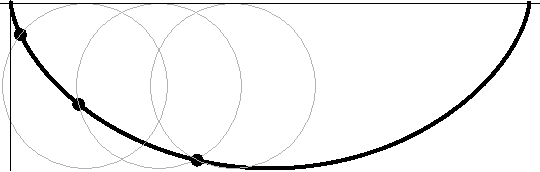
\includegraphics{figures/brachistochrone.pdf}}
\end{center}
\caption{The brachistochrone curve (cycloid) as the trajectory of a point on the boundary of a circle rolling on a line. \label{fig:brachistochrone}}
\end{figure}


\beginexample{Geodesics in the hyperbolic plane} The hyperbolic plane is a well-known example of a \emph{non-Euclidean geometry}, i.e., a geometry in which Euclid's parallel postulate fails to hold. A concrete realization of the hyperbolic plane consists of the set
\eqst{ \mathbb{H} = \{ (x,y)\in \mathbb{R}^2\,:\, y>0 \} }
(known as the \emph{upper half plane} in complex analysis), together with a modified formula for the arc length of a line segment, namely
\eqst{ ds = \frac{\sqrt{dx^2 + dy^2}}{y}, }
which replaces the usual formula $ds = \sqrt{dx^2+dy^2}$ for the ordinary Euclidean arc length. In other words, in the hyperbolic plane, the higher you go, the more ``flat'' in the vertical direction your hyperbolic length measurement becomes, in the sense that you need to traverse $y$ units of ordinary Euclidean distance for each unit of hyperbolic arc length. 

(The hyperbolic plane can also be realized inside a unit disk, resulting in a geometry in which objects seem to shrink---to our Euclidean eyes---as they approach the boundary of the disk. This geometry was famously portrayed by the Dutch artist M.~C.~Escher in a beautiful series of wood engravings; see Figure~\ref{fig:escher}.)

\begin{figure}
\begin{center}
\scalebox{0.25}{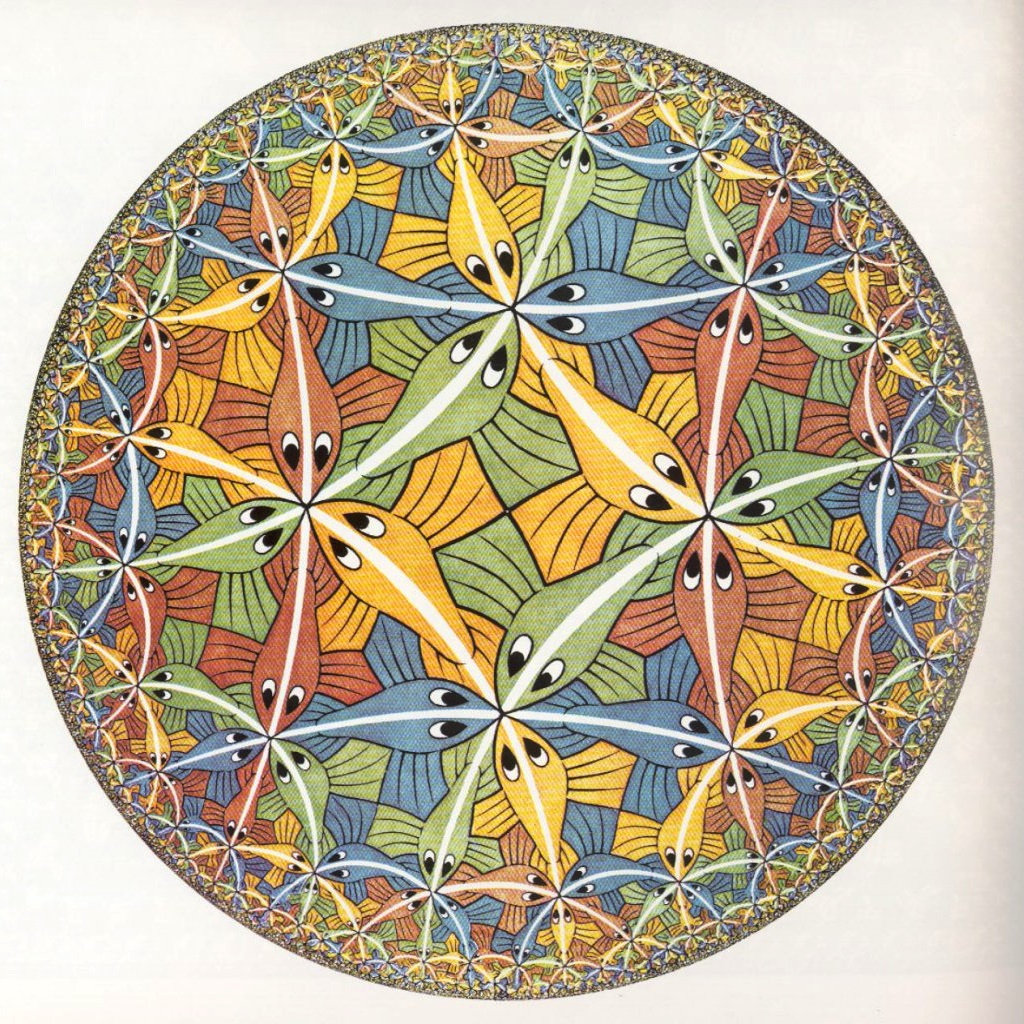
\includegraphics{figures/circlelimit3.jpg}}
\caption{M.~C.~Escher's \textit{Circle Limit III} (1959). \label{fig:escher}}
\end{center}
\end{figure}


Let us use the methods of the calculus of variations to find the hyperbolic geodesics, which are the ``straight lines'' (actually shortest paths) between two points $(x_1,y_1), (x_2,y_2)$ in the hyperbolic plane. Imitating the setup of the plane geodesics example, we are trying to minimize the functional
\eqst{ 
\Phi_{\mathbb{H}} = \int_{x_1}^{x_2} \,ds = \int_{x_1}^{x_2} \frac{\sqrt{1+q'(x)^2}}{q}\,dx 
= \int_{x_1}^{x_2} L_{\mathbb{H}}(q',q)\,dx, 
}
which is expressed in terms of a Lagrangian
\eqst{ 
L_{\mathbb{H}}(q',q) = \frac{\sqrt{1+q'^2}}{q}.
}
The Euler-Lagrange equation becomes
\eqst{
\der{}{x}\left(\frac{q'(x)}{q(x)\sqrt{1+q'(x)^2}}\right)=
\der{}{x}\left(\pder{L_{\mathbb{H}}}{q'} \right) = \pder{L_{\mathbb{H}}}{q} = -\frac{\sqrt{1+q'(x)^2}}{q(x)^2}.
}
After a short computation, this reduces to the equation
\eqst{
1+q'(x)^2+q(x)q''(x) = 0,
}
or
\eqst{
\frac{d^2}{dx^2}\left(\tfrac12 q(x)^2\right)
= \der{}{x}\left(q(x) q'(x)\right) = -1.
}
This is readily integrated, to give
\eqst{
\tfrac12 q(x)^2 = -x^2 + Cx + D,
}
or
\eqst{
q(x) = \sqrt{a^2 - (x-b)^2},
}
where $D=a^2-b^2, C=2b$. The equation $y=q(x)$ is the equation for a semicircular arc that crosses the $y$-axis perpendicularly---these semicircular arcs are the geodesics in the hyperbolic plane. In addition, in the case when $x_1=x_2$, it is easy to verify that the geodesic connecting $(x_1,y_1)$ to $(x_2,y_2)$ will be a vertical straight line. (In the ``unit disk'' version of the hyperbolic plane, the geodesics are circular arcs that intersect the boundary of the disk perpendicularly.)

\beginexer Find a formula for the length (as measured using the hyperbolic metric!) of a hyperbolic geodesic arc between the points $(x_1,y_1), (x_2,y_2)\in \mathbb{H}$.

%\beginexample{Tautochrone problem}


\beginexample{Isoperimetric inequality} The \emph{isoperimetric problem} was the classical problem, discussed already by the ancient Greeks, of finding the simple closed curve in the plane with perimeter $L$ that bounds the largest area (in modern times the problem has been considerably generalized to higher dimensions, curved spaces etc.). The answer is that the so-called \emph{isoperimetric curve} is a circle, and can be derived using the calculus of variations. A slight complication is that the problem involves minimizing a functional (the area bounded by the curve) subject to a constraint (representing the fixed perimeter); this difficulty can be addressed easily using the standard idea of Lagrange multipliers from ``ordinary'' calculus (note the repeated occurrence of the mathematician Joseph Louis Lagrange's name---it is no coincidence, of course).

We model the isoperimetric problem as the problem of minimizing the area functional
\eqst{
A = \int_{x_0}^{x_1} q(x)\,dx
}
among all curves $q(x)$ taking nonnegative values on $[x_0,x_1]$, and satisfying $q(x_0)=q(x_1)=0$ as well as the arc length constraint
\eqst{
\int_{x_0}^{x_1} ds =  \int_{x_0}^{x_1} \sqrt{1+q'(x)^2}\,dx = \ell.
}
Such a curve $q(x)$ represents the ``upper part'' of the closed  curve that lies above the $x$-axis, and meets it at the points $x=x_0, x=x_1$. The solution should be a semicircle meeting the $x$-axis perpendicularly at those points; once this fact is derived, one can derive the claim about circles being the solution to the isoperimetric problem without too much effort, after making reasonable assumptions about the form of the solution. % (see the exercise below).

Since this is an optimization problem under constraints, the technique of Lagrange multipliers requires us to solve the modified \emph{non-constrained} problem of optimizing the functional
\eqst{
A_\lambda = \int_{x_0}^{x_1} q(x) + \lambda \sqrt{1+q'(x)^2}\,dx
= \int_{x_0}^{x_1} L_\lambda(q',q)\,dx,
}
where $L_\lambda$ is a new Lagrangian that is obtained by taking the ``original'' Lagrangian $L=q$ and adding a constant multiple of the constraint function $\sqrt{1+q'^2}$. The price of replacing the constrained problem by an unconstrained one is the introduction of an additional parameter, $\lambda$, known as the \emph{Lagrange multiplier}. After solving the unconstrained problem in terms of the parameter $\lambda$, the requirement for the constraint to be satisfied gives an equation for $\lambda$. (A proof that this technique works is beyond the scope of this course, but the geometric intuition is very similar to the case of Lagrange multipliers in ordinary calculus.)

To see how this idea works in practice, we write the Euler-Lagrange equation $\der{}{x}\left(\pder{L_\lambda}{q'}\right) = \pder{L_\lambda}{q}$ for the unconstrained optimization problem. This gives
\eqst{
\der{}{x}\left( \frac{\lambda q'(x)}{\sqrt{1+q'(x)^2}}\right) = 1,
}
or
\eqst{
\frac{q'(x)^2}{1+q'(x)^2} = (Ax+B)^2,
}
where $A,B$ are constants related to the values of $\lambda$ and an integration constant. 
Solving for $q'$ and then integrating, we get
\eqst{
q'(x) &= \pm \frac{Ax+B}{\sqrt{1-(Ax+B)^2}}, \\
q(x) &= \pm \sqrt{A^{-1}-(x+B/A)^2}+E = \pm \sqrt{C-(x+D)^2} + E,
}
where $C,D,E$ are constants. If we now impose the constraints that $q$ is nonnegative, $q(x_0)=q(x_1)=0$, and assume that the arc length $\ell$ is exactly $\frac{\pi}{2}(x_1-x_0)$, we find that the solution to our optimization problem must have the form
\eqst{
q(x) = \sqrt{\left(\frac{x_1-x_0}{2}\right)^2 - \left(x-\frac{x_1+x_0}{2}\right)^2},
}
which is indeed a semicircular arc that meets the $x$-axis perpendicularly at $x_0,x_1$.

%\beginexer Show that if a closed curve in the plane with given perimeter $\ell$ can be described in terms of two curves $q_-(x) \le 0 \le q_+(x)$ defined on the interval $[x_0,x_1]$ (representing the ``upper'' part and the ``lower'' part of the closed curve), and satisfying $q_-(x_0)=q_+(x_0)=q_-(x_1)=q_+(x_1)=0$, then the total area bounded by the curve is minimized when both $q_-$ and $q_+$ are the semicircles obtained as the solution to the minimization problem discussed above. (Note that this is still not a complete solution to the isoperimetric problem, since we have made various assumptions about the form and smoothness properties of a solution. More elegant solutions of the problem which make no such assumptions can be found in many differential geometry and calculus of variations textbooks.)


\beginexercise{Surfaces of revolution} The surface obtained by taking a curve $y=q(x)$ on some interval $[x_1,x_2]$ and rotating it around the $x$-axis is called the \emph{surface of revolution} of the curve. Its surface area is known to be
\eqst{
S = \int_{x_1}^{x_2} 2\pi y\,ds = 2\pi \int_{x_1}^{x_2} q(x)\sqrt{1+q'(x)^2}\,dx.
}
For given values of $x_1<x_2$ and boundary values $q(x_1)=y_1, q(x_2)=y_2$, find the nonnegative curve that minimizes $S$. The surface of revolution of this famous curve can be physically realized as the shape of a soap film between two circular metal rings (see Figure~\ref{fig:catenoid}).

\begin{figure}
\begin{center}
\scalebox{0.5}{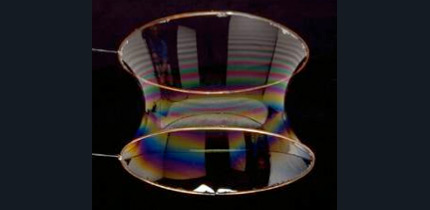
\includegraphics{figures/catenoid.jpg}}
\caption{The catenoid, a minimal surface of revolution. \label{fig:catenoid}}
\end{center}
\end{figure}


\beginexercise{A hanging rope} A rope of length $L$ and uniform linear density $\rho$ hangs between two points $\mathbf{A}=(x_1,y_1)$, $\mathbf{B}=(x_2,y_2)$, where $x_1<x_2$, and clearly we have to assume that $(x_2-x_1)^2+(y_2-y_1)^2 \le L^2$. Its shape is determined by the requirement that the potential energy
$$ E = -\int_{x_1}^{x_2} \rho gy\,ds $$
is minimized. Find the general equation for the shape.

\beginexample{The elastic rod} A thin elastic rod of length $L$ is made to bend as it is clamped horizontally between the two points $(0,0)$ and $(A,0)$ (where $A<L$). Its shape can be determined from the condition that the elastic energy is minimized. The energy is proportional to an integral along the curve of the square of its curvature:
$$ E = \int \tfrac12 J (\textrm{curvature})^2\,ds = \tfrac12 J \int \kappa(s)^2 \,ds, $$
where $J$ is a constant characteristic of the material and geometric cross section of the rod, and $ds$ denotes arc length.
The curvature $\kappa(s)$ at a point along the curve is the reciprocal of the \emph{radius of curvature}, defined as the radius of a circle that can be brought to touch the curve tangentially in such a way that both the first and second derivatives of the curve and circle coincide. 

Let the shape of the rod be described by the functions $(x(s), y(s))$ of the arc length parameter $s$, which varies from $0$ to $L$. Let $\theta=\theta(s)$ be the angle between the positive $x$-axis and the tangent to the curve at the point $(x(s),y(s))$; i.e., we have the relations
\eqst{ \tan \theta = \der{y}{x}, \quad \cos\theta = \der{x}{s}, \quad \sin\theta = \der{y}{s}. }
From elementary geometry it is known that $\kappa(s) = |\der{\theta}{s}|$, i.e., the curvature is the absolute rate of change of the angle of the tangent with arc length [it is also the magnitude of the acceleration vector $(x''(s),y''(s))$]. So, in terms of the angle-arc-length functional representation $\theta(s)$ of the curve, the energy functional can be written as
\eqst{ E = \int_0^L \tfrac12 J \theta'(s)^2 \,ds. }
To derive an ODE for this minimization problem, note that the boundary conditions
\eqst{ 
y(0) = y(L) = x(0)= 0, \ \ \ x(L)=A,
} 
translate to two constraints
\eqst{
\int_0^L \der{y}{s}\,ds = \int_0^L \sin\theta(s)\,ds &= 0, \\
\int_0^L \der{x}{s}\,ds = \int_0^L \cos\theta(s)\,ds &= A.
}
In addition, we have the condition $\theta(0)=\theta(L)=0$.
We therefore need to introduce two Lagrange multipliers $\lambda_1, \lambda_2$, and solve the unconstrained optimization problem for the modified energy functional
\eqst{ E_{\lambda_1, \lambda_2} = \int_0^L \left(\tfrac12 J \theta'(s)^2 - \lambda_1 \sin\theta(s) - \lambda_2 \cos\theta(s)\right)\,ds }
This gives the Euler-Lagrange equation
\eq{ \label{eq:elasticaeq}
J \theta''(s) = -\lambda_1 \cos \theta(s) + \lambda_2 \sin\theta(s).
}
Note that this equation is somewhat similar to the pendulum equation \eqref{eq:pendulumeq}, and indeed can be brought to the form of \eqref{eq:pendulumeq} by replacing the function $\theta(s)$ by a shifted version of it $\varphi(s)=\theta(s)+\alpha$, for a suitable $\alpha$. The curves solving \eqref{eq:elasticaeq} are known as \emph{elastica} curves, and this useful coincidence between the elastica equation and the theory of the pendulum is the starting point for a beautiful analysis of the possible shapes that can be assumed by an elastic rod. We will not go into the details of this analysis here.

\beginexercise{Solid of revolution with least airflow resistance}
The air resistance experienced by a bullet, whose shape is the solid of revolution of a curve $y=q(x)$, moving through the air is
\eqst{ \Phi = 4\pi \rho v^2 \int_0^L q(x) q'(x)^3\,dx, }
where $\rho$ is the density of the material, $v$ is the velocity of motion and $L$ is the length of the body of the bullet. Find the optimal shape $q(x)$ that results in the smallest resistance, subject to the conditions $q(0)=0, q(L)=R$.




\subsection{The phase flow and Liouville's theorem}

Hamiltonian systems often have quantities which are conserved; for example, in autonmous systems we saw that the Hamiltonian itself is conserved. In other cases, if the Lagrangian does not depend on one of the generalized coordinates $q_j$, then $\pder{L}{q_j}=0$, so, by the Euler-Lagrange equation for that coordinate, the generalized momentum $p_j = \pder{L}{\dot{q}_j}$ is a conserved quantity (in such a case we say that $q_j$ is a \emph{cyclic coordinate}). Such invariant quantities lead directly to the usual conservation laws from mechanics---the conservation of energy, of momentum, and of angular momentum---as well as to more exotic conserved quantities that arise in specific problems.

We now discuss a different kind of conserved quantity, one that is associated not with specific solutions, but rather with an entire family of solutions. What we will do is to start with an entire set of initial states in the phase space, then let those states evolve according to the dynamical equations. After some time $t$, the initial states have evolved to occupy some new set in the phase space. It turns out that the total \emph{area} of the set is conserved: this is the statement of Liouville's theorem.

To state the theorem formally, given a Hamiltonian system \eqref{eq:hamiltoniansystem}, for each point $\mathbf{x}=(p_0,q_0)\in\mathbb{R}^2$ and time $t\ge 0$, denote by $\varphi_t(\mathbf{x})$ the point $(p(t),q(t))$, where $(p(t),q(t))$ are the solutions to the equations \eqref{eq:hamiltoniansystem} with initial condition $p(0)=p_0, q(0)=q_0$. (We assume that the system is such that the solutions exist for all time $t\ge 0$.) Thus, for each $t\ge 0$ we have constructed a mapping
$$ \varphi_t:\mathbb{R}^2\to\mathbb{R}^2, $$
which takes a ``present'' point corresponding to the state of the system at time $0$ into a ``future'' point corresponding to the state of the system $t$ units of time later. The family of maps $(\varphi_t)_{t\ge 0}$ is called the \emph{phase flow} of the system: it describes how points ``flow'' along the solution lines of the system.

\begin{thm}[Liouville's theorem] 
The phase flow preserves area. More precisely, given a region $E\subset\mathbb{R}^2$ with finite area, for any $t\ge 0$ we have
\eqst{ 
\operatorname{area}(\varphi_t(E)) = \operatorname{area}(E). 
}
\end{thm}

\begin{proof}
Note that for fixed $t$, there is a one-to-one correspondence between points $(p,q) \in \varphi_t(E)$ and points $(p_0,q_0)\in E$, defined by $(p,q)=\varphi_t(p_0,q_0)$. This smooth map has a Jacobian
\eqst{
J_t = \pder{(p,q)}{(p_0,q_0)},
}
i.e., $J_t$ is the determinant of the Jacobian matrix 
\eqst{
\renewcommand{\arraystretch}{1.5}
\frac{D(p,q)}{D(p_0,q_0)} = \left(\begin{array}{cc}
\pder{p}{p_0} & \pder{p}{q_0} \\ \pder{q}{p_0} & \pder{q}{q_0}
\end{array}\right).
}
The Jacobian factor $J_t$ enters into the area computation via a change of variables in a double integral, as follows:
\eqst{
\operatorname{area}(\varphi_t(E)) &= \iint_{\varphi_t(E)} dp\,dq 
= \iint_E \pder{(p,q)}{(p_0,q_0)}\,dp_0\,dq_0
\\ &= \iint_E J_t \,dp_0\,dq_0.
}
We claim that $J_t\equiv 1$ for all $t$. This will imply that
\eqst{
\operatorname{area}(\varphi_t(E)) &= \iint_{\varphi_t(E)} dp\,dq 
= \iint_E \,dp_0\,dq_0 = \operatorname{area}(E),
}
and therefore finish the proof. It will be instructive to do this by computing $J_t$ more generally for the generic (not necessarily Hamiltonian) planar system
\eqst{
\dot{p} = F(p,q,t), \qquad
\dot{q} = G(p,q,t).
}
Denote 
\eqst{
\renewcommand{\arraystretch}{1.5}
X_t = \frac{D(p,q)}{D(p_0,q_0)} = \left(\begin{array}{cc}
\pder{p}{p_0} & \pder{p}{q_0} \\ \pder{q}{p_0} & \pder{q}{q_0}
\end{array}\right),
}
and observe that, by the chain rule,
\eqst{
\der{X_t}{t} = 
\renewcommand{\arraystretch}{1.5}
\left(\begin{array}{cc}
\pder{\dot{p}}{p_0} & \pder{\dot{p}}{q_0} \\ \pder{\dot{q}}{p_0} & \pder{\dot{q}}{q_0}
\end{array}\right) =
\left(\begin{array}{cc}
\pder{p}{p_0} \pder{F}{p} + \pder{q}{p_0} \pder{F}{q} & \pder{p}{q_0} \pder{F}{p} + \pder{q}{q_0} \pder{F}{q} \\
\pder{p}{p_0} \pder{G}{p} + \pder{q}{p_0} \pder{G}{q} & \pder{p}{q_0} \pder{G}{p} + \pder{q}{q_0} \pder{G}{q}
\end{array}\right)
 = A_t X_t,
}
where
\eqst{
\renewcommand{\arraystretch}{1.5}
A_t = A_t(p_0,q_0) = \left(\begin{array}{cc} \pder{F}{p} & \pder{F}{q} \\ \pder{G}{p} & \pder{G}{q} \end{array}\right).
}
In other words, for fixed $(p_0,q_0)$, the matrix $X_t$ satisfies the time-dependent linear matrix ODE 
\eqst{ \dot{X}_t = A_t X_t, }
with the initial condition $X_0 = I$ (the $2\times2$ identity matrix).

As a consequence, we now claim that the determinant $J_t = \det X_t$ also satisfies an ODE, namely
\eq{ \label{eq:liou-jac-ode}
\dot{J}_t = \operatorname{tr}(A_t) J_t.
}
Indeed, for small positive $h>0$ we have
\eqst{
J_{t+h} &= \det(X_{t+h}) = \det( X_t+h A_t X_t + O(h^2) ) \\ 
&= \det((I+h A_t)X_t+O(h^2))
= \det(I+h A_t) \det(X_t) + O(h^2)
\\ &= (1 + h \operatorname{tr}(A_t)) J_t + O(h^2),
}
where the last step is true because of the exercise below on determinants of perturbations of the identity matrix.
Subtracting $J_t$ from both sides and taking the limit as $h\downarrow 0$ gives
\eqst{
\der{J_t}{t} = \lim_{h\downarrow 0} \frac{J_{t+h}-J_t}{h} = 
\lim_{h\downarrow 0} \left(\operatorname{tr}(A_t)J_t + O(h)\right) = \operatorname{tr}(A_t)J_t.
}
The equation \eqref{eq:liou-jac-ode} is an easy scalar ODE for $J_t$, with the initial condition $J_0=1$. Its solution is
\eq{ \label{eq:liouville-jacobian}
J_t &= \exp\left( \operatorname{tr}\left(\int_0^t A_s\,ds\right)\right)
\\ &= \exp\left[ \int_0^t \left(\pder{F}{p}+\pder{G}{q}\right)\,ds \right]
\\ &= \exp\left( \int_0^t \divr(F,G) \,ds \right).
}
Going back to the case of the Hamiltonian system, we recall that in this case
$$ \divr (F,G) = \pder{F}{p}+\pder{G}{q} = -\frac{\partial^2 H}{\partial p \partial q} + 
\frac{\partial^2 H}{\partial p \partial q} = 0, $$
so we finally get that $J \equiv 1$, as claimed.
\end{proof}

\beginexercise{Determinants of perturbations of the identity matrix} Show that if $A$ is a square matrix then
\eqst{
\der{}{h}{\raisebox{-5pt}{\Big|}_{h=0}} \det(I+h A) = \operatorname{tr}(A),
}
or equivalently
\eqst{
\det(I+h A) = 1 + h \operatorname{tr}(A) + O(h^2).
}

\beginexercise{Matrix exponentials} The exponential $\exp(A)$ of a square matrix $A=(a_{i,j})_{i,j=1}^d$ is defined by
\eqst{ \exp(A) = \sum_{n=0}^\infty \frac{1}{n!} A^n. }
\begin{enumerate}
\item Show that the series converges absolutely in the matrix norm 
\eqst{ \lVert A \rVert = \sum_{i,j} |a_{i,j}|. }
\item Show that the unique solution to the linear vector ODE
\eqst{
\dot{\mathbf{x}} = A \mathbf{x}
}
with initial condition $\mathbf{x}(0) = \mathbf{x}_0$ (where we think of $\mathbf{x}$ as a column vector in $\mathbb{R}^d$) can be expressed in terms of matrix exponentials, namely
\eqst{ \mathbf{x}(t) = \exp\left(t \mathbf{A}\right) \mathbf{x}_0, \qquad t\ge 0. }
\item Use this to explain the characterization of the stability of rest points in a planar system in terms of the eigenvalues of the Jacobian matrix.

\item Prove that if $A, B$ are commuting square matrices (i.e., matrices which satisfy $AB=BA$) then $\exp(A+B)=\exp(A)\exp(B)$.
\end{enumerate}

\beginexercise{Determinant of a matrix exponential}
Prove the formula
\eqst{ \det\left( \exp(A)\right) = e^{\operatorname{tr}(A)}, }
where $A$ is a square matrix and $\operatorname{tr}(A)$ denotes the trace of $A$. 

\medskip \noindent \textbf{Hint.} 
Take determinants of both sides of the equation $\exp(A)=\exp(n^{-1} A)^n$, which is true by part (4) of the exercise above, then use the fact that $\exp(n^{-1} A)=I+n^{-1}A + O(n^{-2})$ and the exercise above on determinants of matrices close to $I$.

\begin{cor} The phase flow of a planar system preserves area if and only if the system is Hamiltonian.
\end{cor}

\begin{proof} We saw in the proof of Liouville's theorem that the preservation of area is determined by the Jacobian $J_t$ of the phase flow: if $J_t \equiv 1$ then the system preserves area; conversely, if $J_t(p,q)\neq 1$ for some $t$ at a point $(p,q)=\varphi_t(p_0,q_0)$, then a small disk of radius $\epsilon$ and area $\pi \epsilon^2$ around $(p_0,q_0)$ is mapped by $\varphi_t$ to a set of area approximately $\pi \epsilon^2 J_t \neq \pi \epsilon^2$, and therefore the phase flow does not preserve area.

To conclude, from the computation in \eqref{eq:liouville-jacobian} it follows that the system preserves area if and only if $\divr(F,G)=0$, and we already showed in Lemma~\ref{lem:hamiltonian-div} that this is equivalent to the system being Hamiltonian.
\end{proof}

\begin{cor} The rest points of an autonomous Hamiltonian system are either saddle points or centers.
\end{cor}

\begin{proof} An asymptotically stable or unstable rest point (which is either a node or a spiral) would imply that the phase flow either contracts or expands small disks around the rest point; by Liouville's theorem, this is impossible.
\end{proof}

\subsection{Poincar\'e recurrence theorem}

Liouville's theorem is the starting point for a set of important investigations into the qualitative behavior of Hamiltonian systems. The following theorem illustrates the kind of conclusions that the theorem will enable us to draw.

\begin{thm}[Poincar\'e recurrence theorem]
\label{thm:poincare-recurrence}
Let $D$ be a bounded region of the plane. Let $\varphi:D\to D$ be a continuous one-to-one map which is area-preserving. Then in any neighborhood $N\subset D$, there exists a point $\mathbf{p}=(p,q) \in N$ such that the sequence of points $(\varphi^k(\mathbf{p}))_{k=0}^\infty$ returns to $N$ infinitely many times. Here, $\varphi^k(\mathbf{p})$ denotes the \emph{$k$th iterate of $\varphi$}, i.e., $\varphi^2(\mathbf{p})=\varphi(\varphi(\mathbf{p})), \varphi^3(\mathbf{p})=\varphi(\varphi(\varphi(\mathbf{p})))$, etc.
\end{thm}

\begin{proof}
The images of the neighborhood $N$ under $\varphi$ are
\eqst{ N, \varphi(N), \varphi^2(N), \varphi^3(N), \ldots }
Since $\varphi$ preserves areas, these are all sets of equal area, which lie in the bounded region $D$. It follows that there must be two of them which intersect (otherwise the total area would be infinite), that is, we have $\varphi^k(N) \cap \varphi^\ell(N) \neq \emptyset$ for some $k>\ell\ge 0$. If $\mathbf{p}_1, \mathbf{p}_2 \in N$ are two points such that $\varphi^\ell(\mathbf{p}_1)=\varphi^k(\mathbf{p}_2)=\varphi^\ell(\varphi^{k-\ell}(\mathbf{p}_2))$, then, since $\varphi$ is one-to-one, we get that $\varphi^{k-\ell}(\mathbf{p}_2)=\mathbf{p}_1$. We have shown that there is a point $\mathbf{p}_2\in N$ and an integer $j>0$ such that $\varphi^j(\mathbf{p}_2)\in N$, i.e., the point returned to $N$ after $j$ iterations. To prove the stronger claim that there is a point that returns to $N$ \emph{infinitely many times}, the idea is to apply the same argument again, replacing $N$ with $N\cap \varphi^j(N)$. This is left as an exercise to the reader.
\end{proof}

In the context of an autonomous Hamiltonian system, Theorem~\ref{thm:poincare-recurrence} becomes applicable (by taking $\varphi=\varphi_s$ for any fixed $s>0$) when there is a set of trajectories that is known to be bounded; for example, trajectories with energy bounded from above in such a way that we know no trajectory can escape to infinity. The conclusion in this case is that in the vicinity of each state of the system included in the bounded region, there are states which, after evolving for some time, will return to the vicinity of the same state.

It should be noted that in all but the simplest possible systems, it is hopeless to solve the equations analytically. Many systems, such as the double pendulum, exhibit an additional complexity to their behavior, known as \emph{chaos}, which makes them even more difficult to analyze in detail. Thus, in many cases obtaining a rough understanding of the system's behavior, using qualitative results such as the Poincar\'e recurrence theorem, is our only hope. Note that Liouville's theorem also holds for Hamiltonian systems with more than one degree of freedom (we will not prove this, but the proof is not much more difficult than the planar case).
%In the next section we discuss briefly some more detailed information of a statistical nature that can sometimes be extracted using Liouville's theorem. This approach will lead us naturally to the subject of \emph{ergodic theory}, which we will discuss later in the course.

\subsection{Liouville's theorem and ``statistical dynamics''}

Another, more quantitative, way in which Liouville's theorem makes it possible to reach a broad understanding of a complicated nonlinear system without being able to describe in detail specific solutions, is by looking at \emph{statistical} behavior. To be more concrete, if $\mathbf{p}(t)$ is a solution curve in $\mathbb{R}^d$ of an autonomous Hamiltonian system with $d$ degrees of freedom, instead of trying to understand in detail the motion of $\mathbf{p}(t)$ through the phase space, we can simply ask about the frequency of time $\mathbf{p}(t)$ spends in any given part of it. That is, for a well-behaved (say, bounded and open) set $A \subseteq \mathbb{R}^2$, we look at the time average
\eqst{
f_A(T) = \frac{1}{T} \int_0^T 1_{\{ \mathbf{p}(t) \in A\}}\,dt,
}
where the integrand is equal to $1$ if $\mathbf{p}(t)\in A$ or $0$ otherwise, and ask whether this quantity
(which might be called the \emph{empirical frequency of visits to $A$}) might converge to an interesting limit (which will be a function of the set $A$) as $T\to\infty$. An ideal situation is one in which the limit does not depend on the initial condition $\mathbf{p}(0)$, and looks like
\eq{ \label{eq:idealdensity}
\lim_{T\to\infty} f_A(T) = f_A^{(\infty)} := \int_A g(\mathbf{p})\,d\mathbf{p}.
}
In this case we will say that the density $g(\mathbf{p})$ describes in some sense the ``ideal'' statistics of the system: by following the trajectory of a single solution for a long time, we will learn about the relative proportion of time spent in each part of the phase space by \emph{any} solution. Such knowledge may have very practical applications. Can we say what the density $g(\mathbf{p})$ might be? Note that the function $f_A^{(\infty)}$ by its definition ought to be invariant under the phase flow, in the sense that for all $t\ge 0$,
\eqst{
f_A^{(\infty)} = f_{\varphi_t(A)}^{(\infty)}
}
(an exercise to the reader: prove this). Liouville's theorem says that $A$ and $\varphi(A)$ have the same volume, i.e.,
\eqst{
\int_A d\mathbf{p} = \int_{\varphi_t(A)} d\mathbf{p},
}
so it is reasonable to guess that if \eqref{eq:idealdensity} holds then the density $g(\mathbf{p})$ might simply be a constant. Again, if a result of this type were true it would give us a very nice and potentially useful insight into the behavior of the system. It turns out that \eqref{eq:idealdensity} in its literal form cannot be true, for the simple reason that the system has a natural conserved quantity, the Hamiltonian (which here for convenience we will call the energy); so, each solution only gets to explore a part of the phase space with a constant energy, and therefore the limit on the right-hand side of \eqref{eq:idealdensity} cannot be independent of the initial condition and must instead necessarily be a function of the initial energy. However, there is a way to work around this slight complication and it does not detract from the usefulness of the statistical approach to analyzing dynamical systems. In fact, the argument we just sketched is the beginning of an area of mathematics called \emph{ergodic theory}, which we will discuss more in detail in the second part of the course.


\subsection{The pendulum equation, falling trees and domino waves}

In this section we show how to obtain an exact solution of the simple pendulum equation
\eqst{
\ddot{\theta} + \frac{g}{\ell} \sin \theta = 0
}
and show several applications of this solution. Unfortunately, the solution involves some exotic special functions that are unfamiliar to most people (possibly even to most mathematicians!)---the elliptic integrals and Jacobi elliptic functions---but it is useful (and entertaining) nonetheless.

\subsubsection{Analytic solution using elliptic integrals}

We derive the solution under the assumption that $\theta(0) = 0$, $\dot{\theta}(0)>0$.
%, and that $\theta$ remains bounded, i.e. $|\theta|\le \pi$ for all $t$. 
Let $\lambda=g/\ell$, so the equation becomes $\ddot{\theta}+\lambda \sin \theta=0$. Conservation of energy gives the equation
\eq{ \label{eq:pendulum-energy-cons}
\tfrac12 \dot{\theta}^2-\lambda \cos \theta = \textrm{const} }
(to verify this, differentiate both sides). For reasons which will become clear soon, denote the integration constant on the right by $\lambda(2k^2-1)$, where $k\ge0$ and use the relation $\cos \theta = 1-2\sin^2\tfrac{\theta}{2}$. This brings 
\eqref{eq:pendulum-energy-cons} to the form
\eq{ \label{eq:pendulum-energy-cons2}
(\dot{\theta})^2 = 4\lambda \left(k^2-\sin^2 \tfrac{\theta}{2} \right).
}
Note that this already makes it easy to plot the phase portrait (in the $\theta$-$\dot{\theta}$ plane, or wrapped around a cylinder, since adding multiples of $2\pi$ to $\theta$ does not change the physical state of the system); see Figure~\ref{fig:pendulum-phasediag}.
\begin{figure}
\begin{center}
\scalebox{0.8}{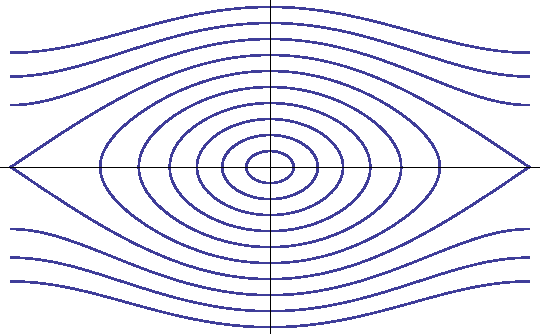
\includegraphics{figures/pendulumphasediag.pdf}} \quad 
\scalebox{0.5}{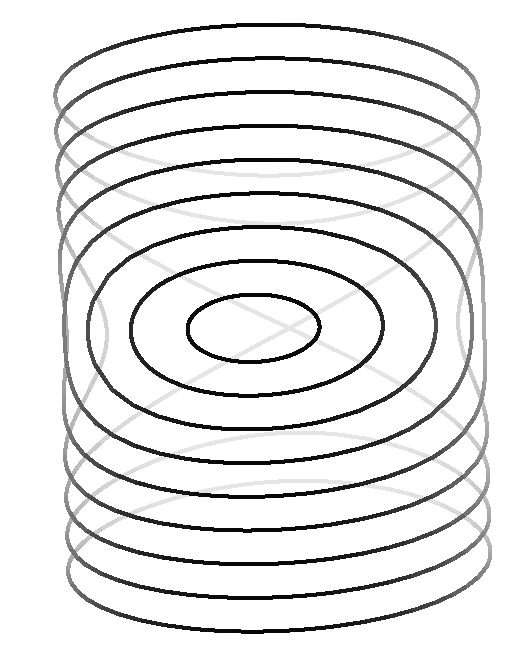
\includegraphics{figures/pendulumphasediag3d.pdf}}
\caption{The phase portrait of the simple pendulum: in the planar representation, the constant energy curves are given by the equation \hbox{$y=\pm 2 \sqrt{\lambda\left(k^2-\sin^2(x/2)\right)}$} for different values of $k$. \label{fig:pendulum-phasediag}}
\end{center}
\end{figure}
The relation between the parameter $k$ and the initial angular velocity $\dot{\theta}(0)$ is found by setting $t=0$ in \eqref{eq:pendulum-energy-cons2}, giving
\eqst{ k=\frac{1}{2\sqrt{\lambda}} \dot{\theta}(0).}
It is also easy to see from the energy conservation equation \eqref{eq:pendulum-energy-cons2} that the periodic solutions (which are the solutions for which $\theta$ remains bounded) correspond to $0<k<1$, and that in that case we have $k=\sin (\theta_{\textrm{max}}/2)$ where $\theta_{\textrm{max}}=\sup_{t\ge 0} \theta(t)$ is the maximal angle that the pendulum will reach (or approach asymptotically, in the case $\theta_{\textrm{max}}=\pi$).
The equation \eqref{eq:pendulum-energy-cons2} is a first-order ODE, and is in a form suitable for separation of variables; e.g., we can write
\eqst{
\frac{d\theta}{\sqrt{k^2-\sin^2 \tfrac{\theta}{2}}} = 2\sqrt{\lambda} \,dt, 
}
or (since we stipulated that $\theta(0)=0$)
\eq{ \label{eq:ellipticintegral-trig}
\int_0^\theta \frac{d\theta}{\sqrt{k^2-\sin^2 \tfrac{\theta}{2}}} = 2\sqrt{\lambda} t.
}
From this point on, assume that $k<1$.
Making the substitution $ku = \sin(\theta/2)$ in the integral on the left, we get the equivalent form
\eqst{
\int_0^u \frac{du}{\sqrt{(1-u^2)(1-k^2 u^2)}} = \sqrt{\lambda} t.
}
The integral on the left is related to a special function known as $\operatorname{sn}(u,k)$ (one of a family of special functions called the \emph{Jacobi elliptic functions}), by
\eqst{
\operatorname{sn}^{-1}(u,k) = \int_0^u \frac{du}{\sqrt{(1-u^2)(1-k^2 u^2)}},
}
(meaning the inverse function of $\operatorname{sn}(u,k)$ as a function of $u$; the variable $k$ is thought of as a parameter, sometimes called the \emph{elliptic modulus}). It follows that
\eqst{
\frac{1}{k}\sin\frac{\theta}{2} = u = \operatorname{sn}(\sqrt{\lambda}t ,k),
}
so finally we get that
\eq{ \label{eq:pendulum-almostfinal}
\sin\frac{\theta}{2} = k \operatorname{sn}(\sqrt{\lambda}t ,k).
}
We have thus obtained our analytic solution, given by the rather intimidating formula
\eqst{
\theta  = 2 \arcsin \left[k \operatorname{sn}(\sqrt{\lambda}t ,k)\right].
}
%This formula is valid also for the parameter values $k>1$ (which correspond to the non-oscillatory solutions where the pendulum has enough energy to ``flip over''), as long as the equation is interpreted as holding ``modulo $2\pi$'', (i.e., considering only the physical state of the pendulum, which corresponds to the geometrical picture of the phase space as a cylinder).

\subsubsection{Formula for the period} 
We can now easily derive a formula for the period of oscillation $T$ of the pendulum. Let $t_{\textrm{max}}$ be the time at which the maximal angle $\theta_{\textrm{max}}$ is attained. We have
\eqst{
k = \sin(\theta_{\textrm{max}}/2) = k \operatorname{sn}(\sqrt{\lambda}\, t_{\textrm{max}},k),
}
so $\operatorname{sn}(\sqrt{\lambda} t_{\textrm{max}},k)=1$, or equivalently,
\eqst{
\sqrt{\lambda}\, t_{\textrm{max}} = \operatorname{sn}^{-1}(1,k) = \int_0^1 \frac{du}{\sqrt{(1-u^2)(1-k^2u^2)}}.
}
The integral on the right-hand side is known as the \emph{complete elliptic integral of the second kind}, and denoted by $K(k)$:
\eqst{
K(k) = \int_0^1 \frac{du}{\sqrt{(1-u^2)(1-k^2u^2)}}.
}
which is also sometimes written as
\eqst{
K(k) = \int_0^{\pi/2} \frac{d\phi}{\sqrt{1-k^2 \sin^2\phi}},
}
using the substitution $u=\sin \phi$.
By symmetry, the period of oscillation of the pendulum is $4t_{\textrm{max}}$ (refer to Figure~\ref{fig:pendulum-phasediag}; the time from $0$ to $t_{\textrm{max}}$ represents a passage around one quadrant in the phase plane). So, we have derived the well-known formula
\eqst{
T= \frac{4}{\sqrt{\lambda}}K(k) = 4\sqrt{\frac{\ell}{g}} K(k)
= 4\sqrt{\frac{\ell}{g}} K(\sin (\theta_{\textrm{max}}/2)).
}
Since $K(0)=\pi/2$, for small values of $\theta_{\textrm{max}}$ we get the approximate formula for small oscillations
\eqst{
T \approx T_0 = 2\pi \sqrt{\frac{\ell}{g}}.
}
Figure~\ref{fig:pendulumperiod} illustrates the dependence of the period on the oscillation amplitude $\theta_{\textrm{max}}$.

\begin{figure}
\begin{center}
\scalebox{0.8}{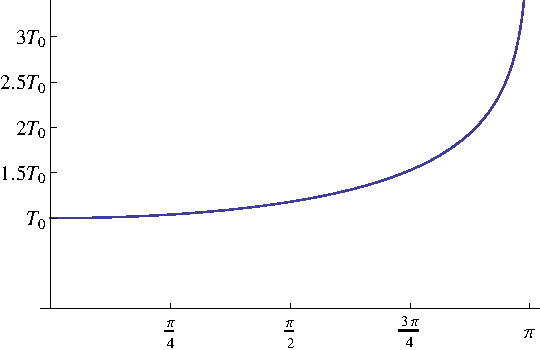
\includegraphics{figures/pendulumperiod.pdf}}
\caption{The period $T$ of a pendulum (measured in units of the period $T_0=2\pi\sqrt{\ell/g}$ for small oscillations) as a function of the oscillation amplitude $\theta_{\textrm{max}}$. \label{fig:pendulumperiod}}
\end{center}
\end{figure}


\subsubsection{Falling time of a tree} A related question concerns the time it takes a vertical standing object such as a tree to fall over from its vertical position once it is given a small destabilizing push. 
This corresponds almost exactly to the pendulum starting from the inverted position $\theta(0)=\pi$, except for the fact that a tree is actually a \emph{compound} pendulum whose mass is distributed in some fashion along its entire length. However, the essential facts remain the same for such a pendulum---one simply has to change the length parameter $\ell$ (see the exercise below, which deals with the case in which the distribution of mass is uniform along the length of the rod on which the pendulum swings). Of course, if the initial angular velocity $\dot{\theta}(0)$ is $0$, then we have an equilibrium state and the tree will not fall over. But this is an unstable equilibrium, so even a tiny non-zero initial angular velocity $\dot{\theta}(0)=\omega_0$ would lead to toppling.

To derive the toppling time, which we denote by $\tau$, observe that the question is equivalent to asking how long it would take for the pendulum starting from the modified initial condition $\theta(0)=0$, $\dot{\theta}(0)=\omega_{\textrm{max}}$ to swing between the angles $\theta=\pi/2$ and $\theta=\pi$, where $\omega_{\textrm{max}}$, the angular velocity at the bottom position $\theta=0$ (which is the maximal angular velocity the pendulum will attain during its motion), is related to $\omega_0$ by the conservation of energy equation
\eqst{
\tfrac12 \omega_0^2 - \lambda \cos(\pi) = \tfrac12 \omega_{\textrm{max}}^2 - \lambda \cos(0),
}
giving the relation $\omega_{\textrm{max}} = \sqrt{\omega_0^2+4\lambda}$.
In other words, using the solution we just derived for just such initial conditions, and specifically \eqref{eq:ellipticintegral-trig}, the quantity we are trying to compute can be written as the difference of two times $\tau = t_2-t_1$, where 
\eqst{
2 \sqrt{\lambda}\, t_1 &= \int_0^{\pi/2} \frac{d\theta}{\sqrt{k^2-\sin^2\tfrac{\theta}{2}}}, \\
2 \sqrt{\lambda}\, t_2 &= \int_0^{\pi} \frac{d\theta}{\sqrt{k^2-\sin^2\tfrac{\theta}{2}}}
}
and $k=\omega_{\textrm{max}}/2\sqrt{\lambda} = \sqrt{1+\frac{\omega_0^2}{4\lambda}}$. 
This can be written succinctly in terms of the special function $K(k)$ and another variant, the \emph{incomplete elliptic integral of the first kind} $F(\alpha, k)$, defined by
\eqst{
F(\alpha,k) = \int_0^\alpha \frac{d\phi}{\sqrt{1-k^2 \sin^2 \phi}}.
}
(Note that $K(k)=F(\pi/2,k)$.) In this notation, we have
\eqst{
\tau &= \frac{1}{2\sqrt{\lambda}} \int_{\pi/2}^\pi \frac{d\theta}{\sqrt{k^2-\sin^2 \tfrac{\theta}{2}}}
= \frac{1}{k \sqrt{\lambda}} \int_{\pi/4}^{\pi/2} \frac{d\phi}{\sqrt{1-k^{-2}\sin^2 \phi}} \\ &=
K(k^{-1}) - F(\pi/4,k^{-1}). 
%= K\left(\sqrt{\frac{4\lambda}{\omega_0^2+4\lambda}}\right)- F\left(\pi/4,\sqrt{\frac{4\lambda}{\omega_0^2+4\lambda}}\right).
}
Note that $\tau$ becomes arbitrarily large when $\omega_0$ approaches $0$.

\beginexercise{Compound pendulum} The falling tree problem is more accurately modeled by a \emph{compound pendulum}, where we assume the mass $m$ is spread out uniformly along the length of the swinging rod, instead of being concentrated at its end. Show that the motion of a compound pendulum with length $\ell$ is equivalent to that of a simple pendulum with length $2\ell/3$.

\subsubsection{The speed of a wave of falling dominoes} \hspace{-5.0pt}\footnote{This section is adapted from the paper \textit{Domino waves} by C.~J.~Efthimiou and M.~D.~Johnson (\textit{SIAM Review} \textbf{49} (2007), 111--120).} If you have ever set up a long chain of dominoes that topple each other in a wavelike progression, you must have wondered how long it would take for all the dominoes to fall once the experiment is set in motion (as everyone knows, it ends all too quickly given the tedious work involved in setting up the dominoes...). We can now answer this question, in a slightly simplified model, using the theory of the pendulum discussed above.

Let us fix some notation for the setup of our domino wave. We assume a row of standing dominoes of height $\ell$ is arranged on a plane, with a fixed horizontal distance of $d$ between each two successive dominoes. For simplicity, we will model each domino as a simple inverted pendulum with mass $m$ (it is not difficult to adapt the analysis to the case of a compound pendulum) and that its thickness is small compared to the inter-domino spacing $d$. We denote by $\beta$ the angle formed between two adjacent dominoes when one rotates around its contact point with the floor until it just touches the other; it is given by
\eqst{
\beta = \sin^{-1}\frac{d}{\ell}.
}
See Figure~\ref{fig:fallingdominoes}.

\begin{figure}
\begin{center}
\begin{picture}(100,120)
%\put(0,20){\line(0,1){100}}
%\put(15,20){\line(0,1){100}}
%\put(0,20){\line(1,0){15}}
%\put(0,120){\line(1,0){15}}
\put(0,20){\dashbox{3}(15,100){\ }}
%%
\put(0,26){\line(0.406737,0.913545){40.67}}
\put(15,20){\line(0.406737,0.913545){40.67}}
\put(0,26){\line(0.913545,-0.406737){15}}
\put(40.6737,117.5){\line(0.913545,-0.406737){15}}
%
\put(56,20){\line(0,1){100}}
\put(71,20){\line(0,1){100}}
\put(56,20){\line(1,0){15}}
\put(56,120){\line(1,0){15}}
%
\put(112,20){\line(0,1){100}}
\put(127,20){\line(0,1){100}}
\put(112,20){\line(1,0){15}}
\put(112,120){\line(1,0){15}}
%
\put(-20,19){\line(1,0){165}}
%
\put(41,10){\vector(1,0){22.5}}
\put(30,10){\vector(-1,0){22.5}}
\put(32.5,7){\scriptsize $d$}
%
%\put(49,11){\vector(1,0){8}}
%\put(22,11){\vector(-1,0){8}}
%\put(22.5,8){\tiny $D-W$}
%
\put(-13.5,67){\scriptsize $\ell$}
\put(-11,65){\vector(0,-1){45}}
\put(-11,75){\vector(0,1){45}}
%
\put(56,110){\Arc(0,0)(0,-26){-25}}
\put(45,73){$\beta$}
\end{picture}
\caption{A row of falling dominoes. \label{fig:fallingdominoes}}
\end{center}
\end{figure}




Our analysis of the speed of the domino wave will be based on analyzing what happens during collisions between dominoes. We will make the following idealized assumptions:
\begin{enumerate}[i.]
\item Only collisions between successive dominoes occur (i.e., we neglect the possible interaction between two dominoes separated by a third domino).
\item The bottom end of each domino is fixed in place by static friction with the floor while it topples, so the domino is only free to rotate around it.
\item Collisions are instantaneous and are elastic, i.e., involve no dissipation of energy: both the energy and momentum of the system are the same \emph{immediately before and after a collision} (of course, during other times energy and momentum are not conserved due to friction forces and dissipation of kinetic energy when dominoes hit the floor).
\end{enumerate}

We will now derive equations relating the initial angular velocity $\omega_0$ of one domino, ``domino $A$'', to the initial angular velocity $\omega_1$ of the next one in the row, ``domino $B$''. Two intermediate quantities that will play a role in the analysis are the angular velocity $\Omega_0$ of domino $A$ \emph{just before} it collides with domino $B$, and its angular velocity $\Omega_1$ \emph{immediately after} the collision. The relationships between the four quantities $\omega_0, \omega_1, \Omega_0, \Omega_1$ are determined by the conservation of energy and momentum.

First, conservation of energy during the motion of domino $A$ from the time it starts to rotate until it hits domino $B$ gives the equation
\eqst{
\tfrac12 m \ell^2 \omega_0^2 + mg\ell = \tfrac12 m \ell^2 \Omega_0^2 + mg\ell \cos \beta,
}
which can be solved for $\Omega_0$ to give
\eq{ \label{eq:dominowave-cons1}
\Omega_0^2 = \omega_0^2 + \frac{2g}{\ell}(1-\cos \beta).
}
Next, conservation of energy during the collision gives
\eqst{
\tfrac12 m\ell^2 \Omega_0^2 = \tfrac12 m\ell^2 \Omega_1^2 + \tfrac12m\ell^2 \omega_1^2,
}
which simplifies to
\eq{ \label{eq:dominowave-cons2}
\Omega_0^2 = \Omega_1^2 + \omega_1^2.
}
To express the conservation of momentum, it is easier (and equivalent) to write an equation for the conservation of \emph{angular} momentum around the base point of domino $B$. This gives
\eqst{
m\ell^2\Omega_0 \cos^2\beta = m\ell^2\Omega_1 \cos^2 \beta + m\ell^2\omega_1.
}
That is,
\eq{ \label{eq:dominowave-cons3}
\Omega_0\cos^2\beta = \Omega_1\cos^2\beta + \omega_1.
}
It is not difficult to solve \eqref{eq:dominowave-cons2}, \eqref{eq:dominowave-cons3} for $\Omega_1$ and $\omega_1$, to get
\eq{ \label{eq:dominowave-cons4}
\omega_1 &= f_+ \Omega_0, \\
\Omega_1 &= \frac{f_+}{f_-} \Omega_0,
}
where
\eqst{
f_{\pm} = \frac{2}{\cos^2 \beta \pm \cos^{-2}\beta}.
}
Plugging the value of $\Omega_0$ obtained from \eqref{eq:dominowave-cons1} into \eqref{eq:dominowave-cons4} finally yields an equation expressing $\omega_1$ in terms of $\omega_0$, namely
\eqst{
\omega_1 = f_+ \sqrt{\omega_0^2 + \frac{2g}{\ell}(1-\cos \beta)} = H(\omega_0).
}
Our analysis has produced the following result: if we start the domino wave going by giving the first domino in the chain a slight push that gives it an initial angular velocity $\omega_0$, then the next domino it will collide with will start its motion with an initial angular velocity equal to $\omega_1=H(\omega_0)$. That domino will collide with a third domino, which will acquire an initial angular velocity of $\omega_2=H(\omega_1)=H(H(\omega_0))$, and so forth: the $n$th domino in the chain will get an initial angular velocity of
\eqst{ \omega_{n-1} = H^{n}(\omega_0) = H(H(H(\ldots H(\omega_0)))\ldots) }
(the $n$th functional iterate of $H$). While it may appear as if the way the wave gets started is important, a more careful look at the properties of the function $H$ shows that in fact the wave will settle down to an equilibrium state in which each domino gets an initial angular velocity equal to
$$ \omega_\infty = \lim_{n\to\infty} \omega_n. 
$$
This equilibrium angular velocity must satisfy the equation
\eqst{ 
\omega_\infty = H(\omega_\infty) = f_+ \sqrt{\omega_0^2 + \frac{2g}{\ell}(1-\cos \beta)},
}
which can be solved to give
\eqst{
\omega_\infty = \frac{2g}{\ell}\frac{f_+^2}{1-f_+^2}(1-\cos\beta) = \frac{2g}{\ell}f_-^2(1-\cos\beta).
}
We are finally ready to answer the original question regarding the speed of a traveling domino wave. Once the wave has reached its equilibrium state, each domino starts its motion with the angular velocity $\omega_\infty$, and rotates through an angle of $\beta$ before colliding with the next domino. By the theory of falling times for the inverted pendulum discussed in the previous section, the time this rotation takes is given by
\eqst{
\tau &= \frac{1}{2\sqrt{g/\ell}} \int_{\pi-\beta}^{\pi} \frac{d\theta}{\sqrt{k^2-\sin^2\tfrac{\theta}{2}}}
= \frac{1}{k\sqrt{g/\ell}} \int_{(\pi-\beta)/2}^{\pi/2} \frac{d\phi}{\sqrt{1-k^{-2}\sin^2 \phi}}
\\ &= \frac{1}{k\sqrt{g/\ell}} \left( K(k^{-1})-F((\pi-\beta)/2,k^{-1}) \right),
}
where
\eqst{
k = \sqrt{\frac{4g/\ell+\omega_\infty^2}{4g/\ell}}.
}
During each such rotation cycle, one can say that the wave has travelled the distance $d$ equal to the inter-domino spacing. Thus, the speed of the domino wave is given by the grand formula
\eqst{
v_{\textrm{wave}} = \frac{d}{\tau} = k d \sqrt{\frac{g}{\ell}}
\left( K(k^{-1})-F((\pi-\beta)/2,k^{-1}) \right)^{-1},
}
Note that all quantities in this formula are expressed as functions of the ``free'' parameters $d, \ell$ and $g$.

\vspace{30.0pt}
\begin{center}
\textbf{End of Part 1}
\end{center}
%
%\vspace{30.0pt}
%
%\section*{Part 2. Discrete-time dynamics, chaos and ergodic theory}
%
%\noindent *** Will be added soon ***
%
%\vspace{30.0pt}
%
%\section*{Part 3. Control theory}
%
%\noindent *** Will be added soon ***
%

%\end{document}

\newpage

\section*{Part 2. Discrete-time dynamics, chaos and ergodic theory}
\addtocounter{section}{1}
\setcounter{subsection}{0}

\subsection{Introduction} \label{sec:ergodic-intro} In this part of the course, we will consider a different flavor of nonlinear systems in which time flows in discrete steps instead of continuously. The set of states of such a system is a set $\Omega$ commonly referred to as the \emph{state space}. In many cases $\Omega$ is a subset of $\mathbb{R}$ or the vector space $\mathbb{R}^d$. The state of the system as a function of time is a sequence $(x_n)_{n=0}^\infty$ of elements of $\Omega$; i.e., it can be thought of as a function of time $n\mapsto x_n$, where the time variable takes only discrete values (and therefore is frequently denoted by the letter $n$ instead of~$t$).

With a continuous-time system, we commonly use an ordinary differential equation $\dot{x}=F(x,t)$ to describe the \emph{dynamics}, i.e., the rules according to which the state of the system evolves. The analogous concept for a discrete-time system $(x_n)_{n\ge 0}$ is called a \emph{difference equation}, which is an equation of the form
\eq{ \label{eq:differenceeq}
  x_{n+1}-x_n &= F(x_n, n),
}
where $F$ is a function $F:\Omega\times \mathbb{N}_0\to\Omega$ (note that this only makes sense if the set $\Omega$ is a subset of a vector space so that the operation of subtraction is defined). Given a state $a \in \Omega$, we can solve the difference equation \eqref{eq:differenceeq} starting from the initial condition $x_0=a$. The solution is obtained (and is easily seen to be unique) by rewriting \eqref{eq:differenceeq} as $x_{n+1}=x_n+F(x_n,n)$ and iterating this ``forward evolution'' rule, e.g.,
\eqst{
x_1 &= x_0 + F(x_0,0), \\ x_2&= x_1+F(x_1,1), \\ x_3&=x_2+F(x_2,2), \ldots 
}
You can see that this process of iteration is much more straightforward than the process of solving ODEs. For example, one does not have to deal with issues of existence or uniqueness of solutions. In fact, in many cases one does not even need to know calculus to work with such equations. On the other hand, as we shall see, many of the other delicate issues that show up in the study of ODEs (such as chaotic behavior, stability and instability, and bifurcations) exist also for difference equations.

\subsection{Difference equations and maps}

As we commented above, the equation \eqref{eq:differenceeq} can be rewritten in a way that eliminates the differencing operation, namely as
\eq{ \label{eq:differenceeq-map}
x_{n+1} &= T(x_n,n),
}
where $T(x_n,n)=x_n+F(x_n,n)$. In many cases the evolution rule of a system is described by giving the function $T:\Omega\times \mathbb{N}_0\to\Omega$ instead of $F:\Omega\times \mathbb{N}_0\to\Omega$; clearly these two descriptions are equivalent, but the latter has the advantage that it makes sense even when $\Omega$ is an abstract set with no extra structure (in which case there is no ``differencing'' operation, so it does not make sense to talk about a difference equation). In the case of the equation \eqref{eq:differenceeq-map}, usually it will be called a \emph{recurrence relation} instead of a difference equation. An especially nice (and very common) situation is one in which $T$ does not depend on the time variable $n$, but instead is simply a function $T(x)$ of the state. In this case \eqref{eq:differenceeq-map} becomes
\eqst{
x_{n+1} &= T(x_n),
}
and the function $T:\Omega\to\Omega$ is called the \emph{evolution map}, or just the \emph{map}, associated with the system; it tells the state of the system one unit of time into the future as a function of the present state. We shall be concerned exclusively with such time-independent systems.

\beginexample{Arithmetic growth} The equation for arithmetic growth is
\eqst{ 
x_{n+1} = x_n + b,
}
where $b\in\mathbb{R}$ is a constant. As a difference equation, it will be written as
\eqst{ x_{n+1}-x_n = b. }
Its solution is the arithmetic sequence $$ x_n = x_0 + bn. $$

\beginexample{Geometric growth} The equation for geometric growth is
\eqst{
x_{n+1} = r x_n ,
}
where $r\in\mathbb{R}$ is a constant, or $x_{n+1}-x_n = (r-1)x_n$ as a difference equation (so, like the ODE $\dot{x}(t)=cx(t)$, it is suitable to model situations in which the rate of change of a quantity is proportional to it). The solution is the geometric sequence $$ x_n = x_0 r^n. $$


\beginexample{Fibonacci numbers} The sequence of Fibonacci numbers $(F_n)_{n=1}^\infty$ is defined as the unique sequence that satisfies the initial conditions $F_1=F_2=1$ together with the recurrence relation
\eq{ \label{eq:recurrence-fibonacci}
  F_{n+2}=F_{n+1}+F_n \qquad (n\ge0).
}
Note that this is a \emph{second-order recurrence relation}---the discrete-time analogue of a second order differential equation. In general, a second-order recurrence will have the form
\eqst{
x_{n+2} &= T(x_n,x_{n+1},n),
}
i.e., each successive value in the sequence is computed as a function of the last two values (and possibly the time parameter). To solve the recurrence we will need to specify not one but two initial conditions, e.g. (if we are trying to solve the recurrence for $n\ge0$) $x_0$ and $x_1$.

It is well-known that the solution to the recurrence \eqref{eq:recurrence-fibonacci} is given by the amusing formula
\eq{ \label{eq:fibonacci-closedform}
F_n = \frac{1}{\sqrt{5}}\left(\frac{1+\sqrt{5}}{2}\right)^n-\frac{1}{\sqrt{5}}\left(\frac{1-\sqrt{5}}{2}\right)^n.
}
This can be proved by induction by verifying the initial conditions and then substituting the expression on the right-hand side into \eqref{eq:recurrence-fibonacci}.

Is there a systematic way to derive such mysterious formulas? As with ODEs, it is often more convenient to represent a second- (or higher-) order system as a first-order system. We can do this by constructing a new system whose state space is $\mathbb{R}^2$ instead of $\mathbb{R}$, where the recurrence relation is given by
\eq{ \label{eq:recurrence-fib-matrix}
\left( \begin{array}{c}X_{n+1}\\Y_{n+1}\end{array}\right) = 
\left( \begin{array}{c} X_n+Y_n \\ X_n
\end{array}\right) = 
\left( \begin{array}{cc}
1&1\\1&0
\end{array}\right) 
\left( \begin{array}{c}X_n\\Y_n\end{array}\right). 
}
Substituting $\left( \begin{array}{c}X_n\\Y_n\end{array}\right)=\left( \begin{array}{c}F_{n+1}\\F_n\end{array}\right)$ into \eqref{eq:recurrence-fib-matrix}, we get
\eqst{
\left( \begin{array}{c}F_{n+2}\\F_{n+1}\end{array}\right)
=
\left( \begin{array}{c} X_{n+1}\\ Y_{n+1}
\end{array}\right) = 
\left( \begin{array}{c} X_n+Y_n \\ X_n
\end{array}\right) =
\left( \begin{array}{c} F_{n+1}+F_n \\ F_{n+1}
\end{array}\right),
}
which reproduces \eqref{eq:recurrence-fibonacci}. Denoting the $2\times 2$ matrix on the right-hand side of \eqref{eq:recurrence-fib-matrix} by $A$, the recurrence relation \eqref{eq:recurrence-fib-matrix} can be thought of as ``geometric growth with a matrix multiplier''. By analogy with the geometric growth example, it is easy to see that its solution is
\eq{ \label{eq:fibonacci-matrixsol}
\left(\begin{array}{c}
F_{n+1}\\F_n 
\end{array}\right) = A^{n-1} 
\left(\begin{array}{c}
1\\1
\end{array}\right).
}
The formula \eqref{eq:fibonacci-closedform} can now be derived using standard diagonalization techniques from linear algebra.

\beginexer Derive the formula \eqref{eq:fibonacci-closedform} by diagonalizing the matrix $A=\left(\begin{array}{cc} 1&1\\0&1\end{array}\right)$ and using the solution \eqref{eq:fibonacci-matrixsol}.

\beginexample{$3x+1$ map} On the state space $\Omega=\mathbb{N}$, define the map $T:\mathbb{N}\to\mathbb{N}$ by
\eqst{
T(x) &= \begin{cases} x/2 & \textrm{if $x$ is even}, \\ 3x+1 & \textrm{if $x$ is odd}.
\end{cases}
}
It is interesting to ask what happens if we start from some initial value $x_0$ and apply the map to get the subsequent values $x_1=T(x_0), x_2=T(x_1)=T(T(x_0)),$ etc. Let's look at some examples:
\eqst{
x=1: \quad & 1\mapsto 4 \mapsto 2 \mapsto 1 \mapsto [\textrm{infinite cycle of }4,2,1], \\
x=3: \quad & 3\mapsto 10\mapsto 5\mapsto 16\mapsto 8 \mapsto 4 \mapsto2\mapsto 1 \mapsto
[\textrm{cycle of }4,2,1], \\
x=6: \quad & 6 \mapsto 3 \mapsto \ldots[\textrm{see above}] \ldots \mapsto [\textrm{infinite cycle of }4,2,1], \\
x=7: \quad & 7 \mapsto 22\mapsto 11\mapsto 34\mapsto 17\mapsto 52\mapsto 26\mapsto13\mapsto40
\mapsto20 \\ & \ \,\mapsto10\mapsto \ldots[\textrm{see above}] \ldots \mapsto [\textrm{infinite cycle of }4,2,1].
}
Is it true that for any initial number $x_0$, iterating the map will eventually reach the infinite cycle $4,2,1$? This famous question, known as the \emph{Collatz problem}, was proposed 75 years ago. Extensive research and numerical computations suggest that the answer is yes, but no one knows how to prove this.

\beginexample{Discretized forward evolution of an ODE} If $\dot{x}=F(x)$ is an autonomous ODE (say on $\mathbb{R}$ or some region of $\mathbb{R}^d$), we can discretize time by allowing it to flow only in integer multiples of some fixed time step $\tau$. That is, we consider the phase flow $(\varphi_t)_{t\ge 0}$ of the system, and for each initial condition $x_0$ define a sequence $(x_n)_{n=0}^\infty$ by
$$ x_n = \varphi_{n\tau}(x_0) \qquad (n\ge 1). $$
Because the phase flow satisfies the equation $\varphi_{t+s}(x)=\varphi_t\circ \varphi_s(x)$, it is easy to see that $x_n$ satisfies the recurrence relation
$$ x_{n+1} = T(x_n),
$$
where $T = \varphi_\tau$. So, the ODE has given rise to a discrete-time dynamical system by fixing the time-step $\tau$.

\beginexample{Poincar\'e section map of an ODE} The time-discretization procedure described in the above example requires an arbitrary choice of a time unit. There is a more natural way to construct a discrete-time dynamical system starting from an ODE that avoids this difficulty, called the \emph{Poincar\'e section map} or \emph{first-return map}. Assume the phase space $\Omega$ of the ODE is $n$-dimensional (i.e., a subset of $\mathbb{R}^n$, or more generally, an ``$n$-dimensional manifold''). Furthermore, assume that there is an $(n-1)$-dimensional subset $A \subset \Omega$ that has the property that all solutions are known to pass infinitely many times through $A$ and through its complement $\Omega\setminus A$. The Poincar\'e map $T:A\to A$ is defined by
\eqst{
T(x) = \varphi_{\tau(x)}(x),
}
where
$\tau(x) = \inf\{ t>0\,:\, \varphi_t(x)\in A\}$ and $\varphi_t:\Omega\to\Omega$ is the phase flow of the system. 

Poincar\'e maps are an extremely useful tool in the analysis of ODEs. A nice illustration of this general construction and its applicability in a specific example is given on page 279 of Strogatz's book \emph{Nonlinear Dynamics and Chaos}.

\beginexample{Logistic map} An important and fascinating example that we will spend a lot of time discussing is the \emph{logistic map} \hbox{$L:[0,1]\to[0,1]$}, a dynamical system with state space $\Omega=[0,1]$. It is actually not one map, but a family of maps $L=L_r$ where $0\le r\le 4$ is a parameter. The map $L_r$ is defined by the formula
\eqst{
L_r(x) = rx(1-x).
}

The logistic map was introduced as a simple model for the fluctuations in the population of a species of animals (or plants, or bacteria etc.) in an environment with limited resources. The idea is that $x$ represents the size of the population (as a fraction of some absolute maximum), and the assumptions are that for small values of $x$, the population will increase in a roughly geometric pattern, but for large values of $x$ the growth will taper off as the animals deplete the available food resources, leading to starvation and a dramatic reduction in population size for even larger values of $x$ (see Figure~\ref{fig:logisticmap}).
\begin{figure}
\begin{center}
\scalebox{0.7}{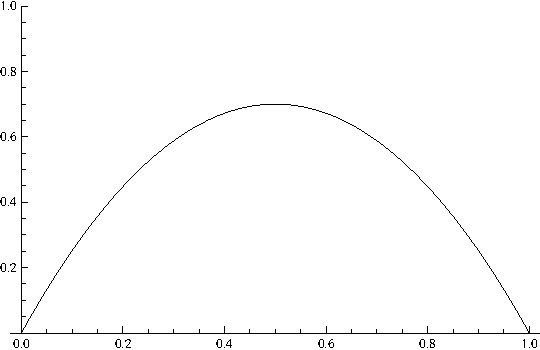
\includegraphics{figures/logisticmap28.pdf}}
\caption{The logistic map $L_r$ for $r=2.5$. \label{fig:logisticmap}}
\end{center}
\end{figure}
The behavior of the logistic map, depending on the value of $r$, can be very simple, or very complicated (or somewhere in between)---in fact, it is one of the simplest examples of a chaotic system, and studying it will give us valuable insights into the more general theory of discrete-time dynamical systems.

\beginexample{Billiard maps} An interesting class of examples with a geometric flavor are the billiard maps. Given some odd-shaped bounded region $D$ in the plane, we let a billiard ball bounce around in $D$, reflecting off the walls without loss of energy. This is a continuous time system, but a standard simplification step is to take its Poincar\'e section map with respect to the set of times at which the ball hits the wall. Thus, the state space of a billiard system considered as a discrete-time system is the set of pairs $(x,\theta)$ where $x \in \partial D$ is a boundary point and $\theta\in [0,2\pi)$ is the angle of the ball's velocity immediately after it reflects off the wall at $x$.

Billiard systems exhibit an extremely rich behavior that is extensively studied by mathematicians and physicists as a toy model for more complicated systems such as the behavior of an ideal gas. Depending on the shape of the ``billiard table,'' the system can have a chaotic structure or a more orderly behavior where nearby initial conditions do not drift far apart. See Figure~\ref{fig:billiards} for some examples.

\begin{figure}
\begin{center}
\begin{tabular}{cc}
\scalebox{0.27}{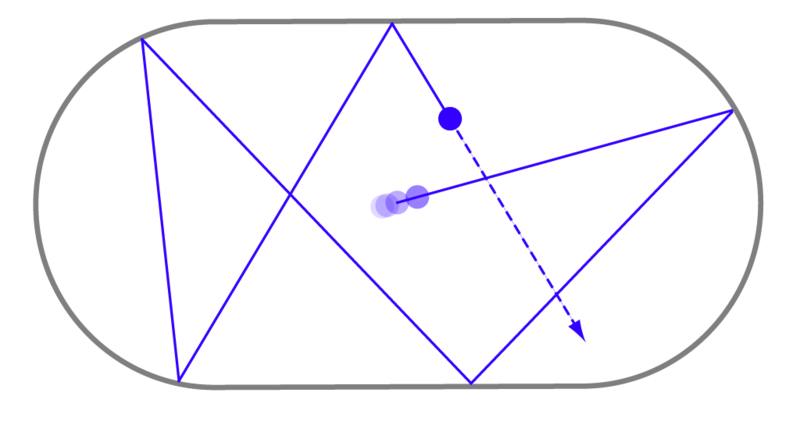
\includegraphics{figures/billiards-bunimovichstadium.png}} &
\scalebox{0.19}{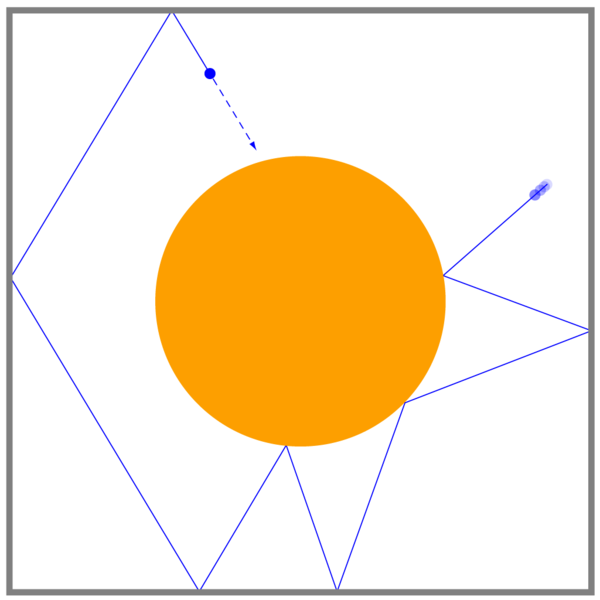
\includegraphics{figures/billiards-sinai.png}} \\  (a) & (b)
\\
\scalebox{0.8}{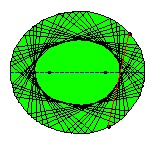
\includegraphics{figures/billiard-ellipse.jpg}} &
\scalebox{0.8}{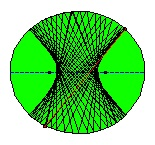
\includegraphics{figures/billiard-hyperbola.jpg}} \\ (c) & (d)
\end{tabular}
\caption{Billiard dynamical systems: (a) The ``Bunimovich stadium''; (b) The ``Sinai billiard'' (source: Wikipedia); (c) and (d) billiard in an ellipse-shaped region.}
\label{fig:billiards}
\end{center}
\end{figure}



\subsection{Interval maps}

A discrete-time system is called \emph{one-dimensional} if it has either $\mathbb{R}$ or a sub-interval of $\mathbb{R}$ as its state space. There are many interesting examples of such systems, and it will be especially convenient to focus on maps defined on an interval, usually taken to be the unit interval $[0,1]$ (or in some cases the open interval $(0,1)$). Such a map is called an \emph{interval map}. The logistic map is one especially interesting example of an interval map. Here are some additional maps that we will consider later.

\beginexample{Doubling map} The doubling map $D:[0,1)\to[0,1)$ is defined by
\eqst{
D(x) &= 2x \textrm{ mod } 1 = \begin{cases}
2x & \textrm{if }0\le x<\tfrac12, \\ 2x-1 & \textrm{if }\tfrac12 \le x < 1, 
\end{cases}
}
(see Figure~\ref{fig:intervalmaps}). As we will see later, it is closely related to binary expansions of real numbers in $(0,1)$. In particular, trying to understand the statistical properties of binary expansions of random numbers leads naturally to questions about properties of the doubling map---see Section~\ref{sec:normalnumbers} for further discussion.

\beginexample{Circle rotation map} For $0<\alpha<1$, the circle rotation map $R_\alpha:[0,1)\to[0,1)$ is defined by
\eqst{
R_\alpha(x) = x+\alpha\textrm{ mod }1
= \begin{cases}
x+\alpha & \textrm{if }0\le x<1-\alpha, \\
x+\alpha-1 & \textrm{if } 1-\alpha \le x\le 1.
\end{cases}
}
The reason for the name of this map is that if one considers the interval $[0,1]$ as a topological circle by identifying the two ends, the map corresponds to a rotation of the circle by the angle $2\pi \alpha$.

\beginexample{Tent map} The tent maps are another one-parameter family of maps $\Lambda_a$, $0<a\le 2$, defined by
\eqst{
\Lambda_a(x) &= \begin{cases}
ax & \textrm{if }0\le x<\tfrac12, \\ a-ax & \textrm{if }\tfrac12 \le x \le 1. 
\end{cases}
}
Figure~\ref{fig:intervalmaps} illustrates the extreme case $a=2$.

\beginexample{Gauss map} Denote by $\{ x \}=x-\lfloor x\rfloor$ the fractional part of a real number $x$ (where $\lfloor x\rfloor = \max\{ n\in\mathbb{Z}\,:\,n\le x\}$ is the integer part of $x$). The Gauss map $G:(0,1)\to[0,1)$, which is related to so-called continued fraction expansions of real numbers, is defined by
\eqst{
G(x) &= \left\{ \frac{1}{x} \right\},
}
i.e., $G(x)=1/x-n$ for $1/(n+1)<x<1/n$, ($n=1,2,\ldots$).

\beginexercise{Properties of the Gauss map}
\begin{enumerate}
\item Show (or read in a number theory textbook how to show) that the numbers $x\in [0,1]$ for which the sequence of iterates $G^n(x)$ eventually reaches $0$ (and is therefore undefined for larger values of $n$) are precisely the rational numbers.

\item Show that the eventually periodic points of $G$ (numbers $x$ for which for some $n$, $G^n(x)$ belongs to an $m$-cycle, see the definition below) are the quadratic irrationals, i.e., the irrational numbers which are solutions of quadratic equations. 

\item Find a formula for all the fixed points of $G$.
\end{enumerate}

\begin{figure}
\begin{center}
\begin{tabular}{cc}
\scalebox{0.6}{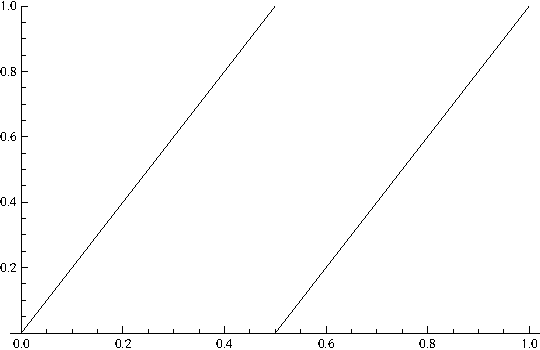
\includegraphics{figures/doublingmap.pdf}} 
&
\scalebox{0.6}{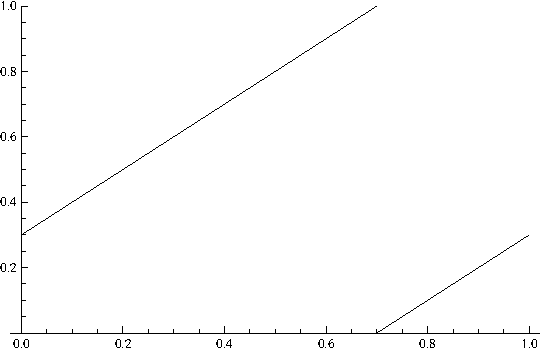
\includegraphics{figures/circlerotation03.pdf}} \\
(a) & (b) \\ 
\scalebox{0.6}{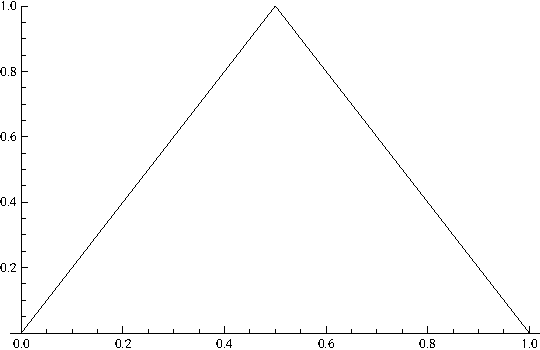
\includegraphics{figures/tentmap.pdf}}
&
\scalebox{0.6}{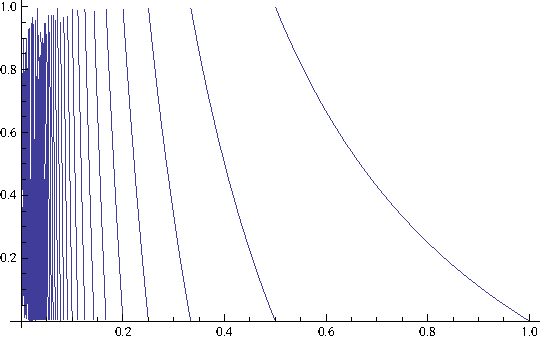
\includegraphics{figures/gaussmap.pdf}} \\ (c) & (d)
\end{tabular}
\caption{(a) The doubling map; (b) The circle rotation map $R_\alpha$ for $\alpha=0.3$; (c) the tent map $\Lambda_2$; (d) The Gauss map.
\label{fig:intervalmaps}}
\end{center}

\end{figure}

\subsection{Fixed points and cycles}

When we studied ODEs, we were interested in rest points, which are static points of the phase state which remain stationary under the ODE dynamics, and in periodic orbits which close in on themselves and lead to infinite repetition of a sequence of movements. In discrete-time systems, the analogous concepts are \emph{fixed points} and \emph{cycles}. A point $x\in I$ is a fixed point of a map $T:I\to\mathbb{R}$ if $T(x)=x$. We call a finite sequence $(x_j)_{j=1}^n$ a cycle (or an $n$-cycle if we want to emphasize its length) of $T$ if all the $x_j$'s are distinct and $T(x_1)=x_2, T(x_2)=x_3, \ldots, T(x_{n-1})=x_n, T(x_n)=x_1$.

The fixed points can be found graphically by drawing the graph of $T$ and the graph of the curve $y=x$, and finding their intersections. Note that if $(x_j)_{j=1}^n$ is an $n$-cycle of $T$ then $x_1 = T(T(T(\ldots(T(x_1)))\ldots)$ (that is, iterating $T$ $n$-times starting from $x_1$ leads back to $x_1$). The map $T$ iterated $n$ times is denoted $T^n$ (usually it is understood from the context that this represents an iteration rather than raising to a power; when there is risk of confusion one needs to be careful and say explicitly what is meant). So, the $n$-cycles can be found by first computing the iterated map $T^n$ and then finding the fixed points of $T^n$. Note that such a fixed point could turn out to be the first point of an $n$-cycle, or it could be a fixed point of $T$, or a fixed point of $T^k$ for some $k<n$ that is a divisor of $n$ (in this case we can use it to generate a $k$-cycle $x_1,T(x_1,\ldots,T^{k-1}(x_1)$). In practice, finding the $n$-cycles often becomes very hard to do when $n$ is larger than some very small number.

\beginexam Consider the map $T(x)=x^2$ on $[0,1]$. The fixed points are solutions of $x^2=x$, i.e., $x=0$ and $x=1$. Computing the iterated maps gives $T^2(x)=T(T(x))=x^4, T^3(x)=x^8, \ldots, T^n(x)=x^{2^n}, \ldots$. The fixed points of $T^n$ are still $x=0$ and $x=1$, which means there are no $n$-cycles for $n>1$.

\beginexam The doubling map $D(x)=2x\textrm{ mod }1$ has no fixed points. What about $2$-cycles? We have $D^2(x)=D(D(x))=4x\textrm{ mod }1$. The equation $x=D(D(x))$ has two solutions: $x_1=4x_1-1$ gives $x_1=1/3$; $x_2=4x_2-2=2/3 = D(x_1)$. So we have found a $2$-cycle $(1/3,2/3)$. In general, it is possible to identify all $k$-cycles, by noting an important connection between the doubling map and the binary expansion of a real number.

\beginexercise{$k$-cycles of the doubling map} Identify all the $k$-cycles of the doubling map, by using the connection with binary expansions (see the discussion in Section~\ref{sec:normalnumbers}). Alternatively, plot $D^k(x)=2^k x \textrm{ mod }1$ and use a graphical approach to identify all the $k$-cycles.

\subsection{Stability of fixed points} What happens to the system $x_{n+1}=T(x_n)$ if we move slightly away from a fixed point $x_*$? We will call the fixed point $x_*$ \emph{asymptotically stable}, or \emph{attracting}, if it has the property that for initial points $x_0$ in some small neighborhood $(x_*-\delta, x_*+\delta)$ of $x_*$, the sequence of iterates $x_n = T^n(x_0)$ converges to $x_*$. We will say that $x_*$ is \emph{asymptotically unstable}, or \emph{repelling}, if there is some $\delta>0$ such that for any initial point $x_0\neq x_*$, the sequence of iterates $x_n=T^n(x_0)$ will eventually leave the interval $[x_*-\delta,x_*+\delta]$. It is also possible for a fixed point to exhibit a mixture of the two types of behavior; for example, it may be attracting for initial points $x_0>x_*$ and repelling for $x_0<x_*$.

To understand the stability properties near a fixed point, consider the linear approximation to $T$ around $x_*$ (assuming it is continuously differentiable in a neighborhood of the fixed point):
\eqst{ T(x) &= T(x_*) + T'(x_*) (x-x_*) + o(x-x_*) \\ &= x_* + T'(x_*) (x-x_*) + o(x-x_*), }
i.e., if the initial point $x_0$ is near $x_*$ then by the neglecting the little-o $o(x-x_*)$ term, we see that for the first few values we have approximately
\eqst{
x_{n+1} - x_* \approx T'(x_*) (x_n-x_*),
}
or, denoting $y_n = x_n-x_*$ and $\lambda=T'(x_*)$,
\eqst{
y_{n+1} \approx \lambda y_n,
}
which is the recurrence for geometric growth. Ignoring the small inaccuracy that comes from the linearization, clearly $y_n\to 0$ if $|\lambda|<1$, and $|y_n|$ becomes larger than some fixed small number $\delta>0$ if $|\lambda|>1$. Thus, we have essentially proved the following fact.

\begin{lem} \label{lem-fixedpoint-stability}
For a fixed point $x_*$, if $|T'(x_*)|<1$ then the fixed point is asymptotically stable, and if $|T'(x_*)|>1$ then the fixed point is asymptotically unstable.
\end{lem}

\beginexer Complete the argument sketched above to get a rigorous proof of Lemma~\ref{lem-fixedpoint-stability}.

\beginexam In the example above involving $T(x)=x^2$, we have $T'(0)=0$ and $T'(1)=2$, so $0$ is an asymptotically stable fixed point, and $1$ is an asymptotically unstable fixed point.

\beginexam Pull out a pocket calculator and repeatedly press the ``$\cos$'' button.
 The value on the display will converge to the number $x_*\approx0.739085$, which is the unique fixed point of $T(x)=\cos x$. Note that $T'(x_*)=-\sin(x_*)\approx -0.673$, which shows that the fixed point is asymptotically stable. Note that the fact that $T'(x)<0$ means that the values of $x_n=\cos^n(0)$ will oscillate around $x_*$, producing values that are alternately bigger and smaller than $x_*$.

\beginexer In the case in which $|T'(x_*)|=1$ but $T''(x_*)\neq 0$, characterize the asymptotic stability of the fixed point as a function of $T'(x_*)$ and $T''(x_*)$.


\subsection{A detailed study of the logistic map}

This section is based on sections 10.2--10.5 in Strogatz's book \emph{Nonlinear Dynamics and Chaos}.

\subsection{Measures and measure preserving maps}

Our study of maps so far has shown that even very simple maps such as the logistic map or the $3x+1$ map can lead to extremely complicated behavior of the associated dynamical system. Is there any hope of understanding such complicated systems in some meaningful sense? Yes, there is. A key insight is that one should focus on questions of a statistical nature: instead of trying to predict in detail where the orbit of a particular initial point $x_0$ will go (which is hopeless for a chaotic system), instead we will try to make predictions about statistical behavior of orbits, i.e., how often they visit each part of the state space. The mathematical object that encodes such a set of statistics is called a \emph{probability measure}, and as we will see, a natural condition for a measure to encode the correct information about a map is that the map is \emph{measure preserving}.

Let $\Omega$ be a set. The theory of probability measures can be developed in much greater generality, but for our purposes we will assume that $\Omega$ is a connected open (or closed) subset of $\mathbb{R}$ or of $\mathbb{R}^d$. Thus, on $\Omega$ there is a natural ``measure'' $d\mathbf{x}$ of $d$-dimensional volume familiar from multivariate calculus. The probability measures that we will consider take the form
$$ P(d\mathbf{x})=f(\mathbf{x})\,d\mathbf{x} $$
where $f$ is a nonnegative function such that $\int_{\Omega} f(\mathbf{x})\,d\mathbf{x} = 1$. Formally, the measure $P$ is considered to be a function $A\mapsto P(A)$ that takes a subset $A\subset \Omega$ and returns a number
$$ P(A) = \int_A f(\mathbf{x})d\mathbf{x}. $$
Both the function $f$, called the \emph{probability density function} associated with $P$, and the set $A$ are assumed to be sufficiently well-behaved that $P(A)$ is defined. (You can learn about the precise technical definitions, which we will not discuss here, in an advanced class on real analysis, measure theory or probability theory). A set $A$ for which $P(A)$ is defined is called a \emph{measurable set}. It is an annoying fact of life that not all sets are measurable, but in practice all sets that you are ever likely to encounter will be measurable, so we will not worry about that.

Now, if $T:\Omega\to \Omega$ is a map and $P$ is a probability measure on $\Omega$, we say that $T$ \emph{preserves the measure $P$} (or \emph{is measure preserving for $P$}) if for any measurable set $A$ the following identity holds:
$$ P(A) = P(T^{-1}(A)), $$
that is,
$$ \int_A f(\mathbf{x})d\mathbf{x} = \int_{T^{-1}(A)} f(\mathbf{x})d\mathbf{x}.
$$
For interval maps, it is sufficient to prove this when $A$ is an interval. The intuitive meaning of the definition is that if the measure $P$ represents the statistical distribution of a random element $x$ in $\Omega$ (corresponding to the state of the dynamical system at some time $n$), then $T(x)$, which corresponds to the state at time $n+1$, will have the same statistical distribution. In other words, the probabilistic behavior is stationary with respect to the time dynamics. A dynamical system $(\Omega, T)$ together with a probability measure $P$ that is preserved by $T$ is called a \emph{measure preserving system}. If $T$ preserves the measure $P$, we say that $P$ is an \emph{invariant measure} for $T$.

\beginexample{Circle rotation map} The circle rotation map $R_\alpha$ preserves the standard length measure on $[0,1)$ (which in analysis is called \emph{Lebesgue measure}---pronounced like \emph{le-baig}), i.e., the measure with density $f(x)\equiv 1$.

\begin{proof} This fact is obvious if you think of the intuitive meaning of the circle rotation map, but for illustration purposes here is a formal proof. If $A$ is a subset of $[\alpha,1)$ then $R_\alpha^{-1}(A) = A-\alpha$, so clearly the length measure is preserved. Similarly, if $A \subset [0,\alpha)$ then $R_\alpha^{-1}(A) = A+1-\alpha$ and again the length measure is preserved. For a general $A\subset[0,1)$, write $A$ as a disjoint union $A=A'\sqcup A''$ where $A'\subset[0,\alpha)$, $A''\subset[\alpha,1)$, then $R_\alpha^{-1}(A) = R_\alpha^{-1}(A')\sqcup R_\alpha^{-1}(A'')$ has the same Lebesgue measure as $A$.
\end{proof}

\beginexample{Doubling map} The doubling map also preserves Lebesgue measure.

\begin{proof}
$$ P(D^{-1}(A)) = 
P\left(\tfrac12 A \sqcup \left(\tfrac12 A+\tfrac12\right) \right)
 = \tfrac12 P(A)
 + \tfrac12 P(\tfrac12+A) =
P(A).
$$
\end{proof}


\beginexercise{Tent map $\Lambda_2$} Show that the tent map $\Lambda_2$ (the special case $a=2$ of the family of tent maps $\Lambda_a$) preserves Lebesgue measure.

\beginexample{Logistic map $L_4$} For $r=4$, the logistic map $L_r=L_4$ preserves the measure
$$ P(dx) = \frac{1}{\pi \sqrt{x(1-x)}}\,dx. $$

\begin{proof} Denote $f(x)=\frac{1}{\pi \sqrt{x(1-x)}}$.
If $A \subset [0,1]$ is an interval, then
\eqst{
P(L_4^{-1}(A)) &= \int_{L_4^{-1}(A)} f(x)\,dx \\ &= 
\int_{L_4^{-1}(A)\cap\left[0,1/2\right]} f(x)\,dx + 
\int_{L_4^{-1}(A)\cap\left[1/2,1\right]} f(x)\,dx
\\ &= \int_A f(\lambda_1(y))\frac{dy}{L_4'(\lambda_1(y))} + \int_A f(\lambda_2(z)) \frac{dz}{-L_4'(\lambda_2(z))},
}
where we define $\lambda_1(y)=\tfrac12(1-\sqrt{1-y}), \lambda_2(z)=\tfrac12(1+\sqrt{1-z})$ (the functions $x=\lambda_{1,2}(w)$ are the two solutions of the equation $L_4(w)=x$), and we make the substitutions
\eqst{
y&=L_4(x) \leftrightarrow x=\lambda_1(y) \textrm{ in the first integral,} \\ z&=L_4(x) \leftrightarrow x=\lambda_2(z) \textrm{ in the second integral}.
}
Note that $L_4$ is decreasing on $[1/2,1]$, which explains why we needed to insert a minus sign in front of the $L_4'(\lambda_2(z))$ term in the second integral.

Now, since we are trying to prove that the expression above is equal to $P(A)=\int_A f(x)\,dx$, it will be enough to show that the following identity holds:
\eqst{
f(x) = f(\lambda_1(x))\frac{1}{|L_4'(\lambda_1(x))|} + f(\lambda_2(x))\frac{1}{|L_4'(\lambda_2(x))|}
}
(the absolute value signs make the sum on the right more symmetric, though of course the first one is unnecessary). This identity is strange but easy to verify: noting the simple relations
\eqst{
L_4'(w) &=4(1-2w), \\ f(w)&=\frac{2}{\pi\sqrt{L_4(w)}}, \\ L_4(\lambda_1(x)) &= L_4(\lambda_2(x)) =x,
}
the right-hand side of the identity becomes
\eqst{
\frac{2}{\pi \sqrt{x}} &\cdot \frac{1}{4(1-(1-\sqrt{1-x}))}
- 
\frac{2}{\pi \sqrt{x}}\cdot \frac{1}{4(1-(1+\sqrt{1-x}))}
\\ & =
\frac{1}{2\pi} \left( \frac{1}{\sqrt{x}}\cdot \frac{1}{\sqrt{1-x}} + 
\frac{1}{\sqrt{x}}\cdot \frac{1}{\sqrt{1-x}} \right) = \frac{1}{\pi\sqrt{x(1-x)}} = f(x).
}
\end{proof}

The idea used in the proof above can be generalized to give a criterion for checking whether a map is measure-preserving.

\begin{lem} \label{lem:measure-pres}
Let $T:I\to I$ be an interval map that is piecewise smooth and monotonic, i.e., the interval $I$ can be decomposed into a union of finitely many subintervals on each of which $T$ is smooth and monotonic (in fact, the claim is true even if this is true for a subdivision into countably many subintervals). Then $T$ preserves the measure $P(dx)=f(x)dx$ if and only if the density $f(x)$ satisfies the equation
\eqst{
f(x) = \sum_{y\in T^{-1}(x)} \frac{f(y)}{|T'(y)|}
}
for all but countably many points $x\in I$, where the sum ranges over all pre-images of $x$.
\end{lem}

\beginexer Prove Lemma~\ref{lem:measure-pres}.


\beginexample{Gauss map} The Gauss map $G(x)$ preserves the measure $\gamma$ on $(0,1)$ (called \emph{Gauss measure}), defined by
$$ \gamma(dx) = \frac{1}{\log 2}\cdot \frac{1}{1+x}\,dx. $$

\beginexer Use Lemma~\ref{lem:measure-pres} to prove this.

\beginexercise{Additive Gauss map} The additive Gauss map $g:[0,1]\to[0,1]$ is defined by
\eqst{
g(x) = \begin{cases} \frac{x}{1-x} & \textrm{if }0\le x\le \tfrac12, \\
\frac{1-x}{x}&\textrm{if }\tfrac12\le x\le 1
\end{cases}
}
(see Figure~\ref{fig:gaussppt}(a)). Show that $g$ preserves the measure 
$$m(dx)=\frac{1}{x}\,dx.$$
(Note: this measure is not a probability measure, since the integral of the density is infinite. However, the concept of measure-preservation makes sense for such measures, and Lemma~\ref{lem:measure-pres} is still valid in this context.)

\beginexercise{Boole map} Show that \emph{Boole's transformation}
\eqst{
B(x)=x-\frac{1}{x}
}
preserves Lebesgue measure on $\mathbb{R}$.


\beginexercise{Pythagorean triples map} The interval map $N:[0,1]\to[0,1]$
\eqst{
\begin{cases}
\frac{x}{1-2x} & \textrm{if }0\le x\le \tfrac13, \\
\frac{1}{x}-2 & \textrm{if }\tfrac13 \le x \le \tfrac12, \\
2-\frac{1}{x} & \textrm{if }\tfrac12 \le x \le 1,
\end{cases}
}
arises in the study of Pythagorean triples. (Figure~\ref{fig:gaussppt}(b) explains why it is denoted by $N$.) Show that it preserves the measure
\eqst{
\pi(dx) = \frac{1}{x(1-x)}\,dx.
}

Although much of our discussion has been focused on interval maps, the concept of measure preserving systems appears in many different contexts (including some rather exotic ones), as the next few examples illustrate.

\begin{figure}
\begin{center}
\begin{tabular}{cc}
\scalebox{0.6}{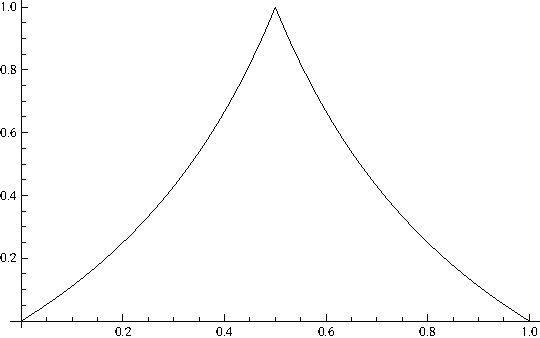
\includegraphics{figures/slowgauss.pdf}}
&
\scalebox{0.6}{
\includegraphics{figures/pythagorean}}
\\
(a) & (b)
\end{tabular}
\caption{(a) The additive Gauss map; (b) The Pythagorean triples map. \label{fig:gaussppt}}
\end{center}
\end{figure}


\beginexample{Hamiltonian flow} By Liouville's theorem, the phase flow of a Hamiltonian system preserves area measure in $\mathbb{R}^2$ (also called the two-dimensional Lebesgue measure). This is a continuous-time dynamical system, but the notion of  measure preserving dynamics makes sense for such systems as well. In particular, if the system is discretized by fixing a time step $\tau$, we get a map preserving Lebesgue measure.

\beginexample{Geodesic flow} The geodesic flow is a continuous-time dynamical system on a curved surface. Its phase space is the set of points $(x,v)$ where $x$ is a point on the surface and $v$ is a tangent vector to the surface based at $x$ (representing the direction and speed in which a person standing at $x$ will start walking). The flow $\varphi_t(\cdot,\cdot)$ takes such a pair $(x,v)$ and maps it to a new pair $(x',v')=\varphi(x,v)$ representing where the person will be, and which direction they will be pointing at, $t$ time units later. It can be shown that the geodesic flow preserves the natural volume measure associated with the phase space (roughly speaking, the measure is product of the surface area measure of the surface in the component $x$, and a standard area measure in the $v$ component).

\beginexample{Billiard map} Billiard maps can be thought of as a limiting case of certain Hamiltonian systems (think of a limit in which the reflecting wall is actually a strongly repelling potential well that becomes steeper and steeper), so they too have an invariant measure. In certain natural coordinates $\phi, \theta, \ell$, the formula for the invariant measure becomes
\eqst{ P(A) = \int_A \frac{\sin \theta}{\sin \theta_1}\, d\theta\, d\phi\, d\ell. }
(For the meaning of these quantities, see the interesting article \emph{What is the ergodic theorem?}, G.~D.~Birkhoff, \textit{American Math. Monthly}, April 1942.)

\beginexample{$3x+1$ map} One of the many (ultimately unsuccessful) attempts at solving the famous $3x+1$ problem mentioned in Section~\ref{sec:ergodic-intro} was based on the observation that since the formula of the $3x+1$ map $T(x)$ depends on the parity of $x$, the range of definition of $T$ can be expanded to include numbers of the form
\eqst{
a_0 + a_1 \cdot 2 + a_2 \cdot 4 + a_3\cdot 8 + \ldots + a_n \cdot 2^n + \ldots = \sum_{n=0}^\infty a_n 2^n.
}
Such exotic numbers, which have an infinite binary expansion to the \emph{left} of the ``binary point'', are called \emph{$2$-adic integers} and have fascinating properties. In particular, there is a natural measure associated with them that is analogous to Lebesgue measure on $\mathbb{R}$. It can be shown that the extended $3x+1$ map preserves this measure.

\subsection{Measure $0$ sets}

A set $E\subset \mathbb{R}$ is called a \emph{measure 0} set if its Lebesgue measure is 0. Although we have not discussed (and do not plan to discuss) precise definitions of Lebesgue measure or of the notion of measurability, for the case of measure 0 sets there is an easy explicit definition. $E$ has measure 0 if and only if for any $\epsilon>0$, $E$ can be covered by a countable union of open intervals whose lengths add up to less than $\epsilon$:
$$ \forall \epsilon>0\ \ \ E\subset\bigcup_{n=1}^\infty (a_n, b_n), \ \  \sum_{n=1}^\infty (b_n-a_n) < \epsilon \ \iff \ \textrm{measure 0.}$$

\beginexer Prove that any countable set $E\subset \mathbb{R}$ has measure~0.

\subsection{Invariant sets, ergodicity and the ergodic theorem}

We now come to a key idea that underlies the basis for all of ergodic theory and explains the importance of invariant measures in discrete-time dynamics. Given a map $T:I\to I$ and the associated recurrence $x_{n+1}=T(x_n)$, for every sub-interval $A\subset I$ we can compute the frequency of visits of the dynamical system to $A$, namely
\eqst{
\mu_{x}^{(n)}(A) = \frac{1}{n} \# \left\{ 0\le k \le n-1\,:\, T^k(x) \in A \right\}.
}
Note that this depends on the set $A$ as well as on $n$ (the number of elements in the sequence of iterates we are using to compute the frequency) and $x$, the initial point. If we fix $n$ and $x$, the function $A\mapsto \mu_x^{(n)}(A)$ is a probability measure (but it is a discrete probability measure, which assigns a positive measure of $1/n$ to the specific points
$x,T(x),\ldots,T^{n-1}(x)$, instead of the measures we considered earlier which were defined in terms of a density function $f(x)$). Now let $n\to\infty$ (for fixed $x$). If we are lucky, the probability measures $\mu_x^{(n)}(\cdot)$ will converge to a limiting measure $P(dx)=f(x)dx$, in the sense that
\eqst{
\mu_x^{(n)}(A) \xrightarrow[n\to\infty]{} P(A) = \int_A f(x)\,dx \ \ \textrm{ for any subinterval }A\subset I.
}
It is not hard to see that the limiting measure needs to be an invariant measure for $T$:
\eqst{
P(T^{-1}(A)) &= \lim_{n\to\infty} \mu_x^{(n)}(T^{-1}(A)) \\ &
= \lim_{n\to\infty} \frac{1}{n}\#\left\{ 0\le k\le n-1\,:\,T^k(x)\in T^{-1}(A) \right\}
\\ &
= \lim_{n\to\infty} \frac{1}{n}\#\left\{ 0\le k\le n-1\,:\,T^{k+1}(x)\in A \right\}
\\ &
= \lim_{n\to\infty} \frac{1}{n}\#\left\{ 1\le k\le n\,:\,T^{k}(x)\in A \right\}
\\ &
= \lim_{n\to\infty} \frac{1}{n}\#\left\{ 0\le k\le n-1\,:\,T^{k}(x)\in A \right\} = P(A).
}

It is therefore clear that an invariant measure which arises in this way encodes useful statistical information about the orbit of the point $x$ under the map $T$. On the other hand, the limiting measure may depend on $x$ (or we may have convergence to a limiting measure for some values of $x$, and fail to have convergence for other values). It turns out that for a wide family of maps, called \emph{ergodic} maps, the limit is mostly independent of the initial point $x$. We summarize the relevant facts, whose proof is beyond the scope of the course, in the following result, which is a version of a famous theorem known as Birkhoff's Pointwise Ergodic Theorem:

\begin{thm}[The ergodic theorem] If $T:I\to I$ is an interval map which preserves a measure $P(dx)=f(x)dx$, then:
\begin{enumerate}
\item There is a set $E\subset I$ such that $I\setminus E$ is a measure-$0$ set and for any $x\in E$, the measures $\mu_x^{(n)}(\cdot)$ converge to a limiting invariant measure $P_x$ in the sense described above.
\item If $T$ satisfies a natural condition known as ergodicity, then $P_x$ is independent of $x$ and is equal to the invariant measure $P$ for all $x\in E$.
\end{enumerate}
\end{thm}

Maps for which the condition of part (b) applies are the ergodic maps. In such a case, one can say that ``the statistics of most orbits reproduce the ideal statistics of the system'', or that ``time averages are equal to space averages''. That is, by observing a typical orbit for a long time we can learn about the statistical behavior of almost all other orbits. We will not discuss the precise definition of ergodicity, preferring instead to explore some of the interesting consequences of the result above. Roughly speaking (setting aside some nuances involving measure 0 sets), a map is ergodic if $I$ can't be divided into two disjoint parts $A$ and $B$ such that $P(A)>0$, $P(B)>0$ and for any points $x\in A, y\in B$, $T^k(x)\in A$ and $T^j(y) \in B$ for all $j,k\ge 0$. Such sets $A$ and $B$ are called \emph{invariant sets} for $T$. The existence of a nontrivial invariant set is a fairly obvious obstacle to the statement of part (b) in the theorem above holding true, and the main difficulty in proving the result is showing that when there are no invariant sets then (in some sense) there is nothing else that can go wrong and therefore the result must be true.

Another thing to note is that actually checking whether a given map is ergodic may be rather difficult. However, we will use the theorem in a few cases in which ergodicity is known and not very difficult to prove.

\subsection{The doubling map and normal numbers}
\label{sec:normalnumbers}

Our first application of the ergodic theorem is related to the doubling map $D(x)=2x\textrm{ mod }1$, which as we have seen preserves Lebesgue measure on $(0,1)$. We will use without proof the fact that this map is ergodic. The reason this is interesting is because the orbits $D^n(x)$ of a number $x$ encode information about the binary expansion of $x$. More precisely, write
\eqst{ x = \sum_{n=1}^\infty a_n(x) 2^{-n},
}
where $a_n(x) \in \{0,1\}$ is the $n$th digit in the binary expansion of $x$ (in the case of a dyadic number $m/2^N$ for which there is a small amount of ambiguity, choose the expansion which terminates with an infinite succession of $0$'s). Applying the doubling map gives
\eqst{
D(x) = 2x\textrm{ mod 1} = \sum_{n=1}^\infty a_n(x) 2^{-(n-1)} \textrm{ mod }1 = \sum_{n=1}^\infty a_{n+1}(x)2^{-n},
}
from which we conclude that $a_n(D(x)) = a_{n+1}(x)$ -- in terms of the binary expansion, the doubling map has the effect of ``chopping off'' the leading digit in the expansion. Successive applications of $D$ will chop off additional digits. By tracking the frequency of visits of $D(x)$ to a specific set such as $(0,1/2) = \{ u\in(0,1)\,:\, a_1(u)=0 \}$, we can prove the following result:

\begin{thm} All numbers $x\in(0,1)$ except those lying in some measure-0 set have the property:
\eq{ \label{eq:normal1}
\frac{1}{n}\#\left\{ 1\le k\le n\,:\, a_n(x) = 0 \right\} \xrightarrow[n\to\infty]{} \tfrac12,
}
and, more generally, for any $b_1,\ldots,b_m\in\{0,1\}$, we have
\eq{ \label{eq:normal2}
\frac{1}{n}\#\left\{ 1\le k\le n\,:\, a_k(x) = b_1,\ldots, a_{k+m-1}(x)=b_m \right\} \xrightarrow[n\to\infty]{} \frac{1}{2^m}.
}
\end{thm}

\begin{proof}
The frequency on the left-hand side of \eqref{eq:normal1} is what we denoted earlier by $\mu_x^{(n)}((0,1/2))$ (with respect to the doubling map), so by the ergodic theorem, it converges to $P((0,1/2))=1/2$. Similarly, the left-hand side of \eqref{eq:normal2} converges to the Lebesgue measure of the interval $[\sum_{j=1}^m b_j 2^{-j},\sum_{j=1}^m b_j 2^{-j}+2^{-m})$, which is $1/2^m$.
\end{proof}

A number $x\in (0,1)$ is called \emph{normal to base $2$} if it satisfies the condition \eqref{eq:normal2}---that is, if its binary expansion contains the digits 0 in 1 in the right asymptotic frequency of $1/2$, and similarly contains each of the types of successive pairs ``$00$'', ``$01$'', ``$10$'' and ``$11$'' with asymptotic frequency $1/4$, each triple of digits with frequency $1/8$, etc. In other words, the binary expansion of a number that is normal to base $2$ is hard to distinguish (at least based on statistics) from the output of an ideal random number generator. We proved above that ``almost every'' $x\in (0,1)$ (all $x$ except for those in some measure-$0$ set) is normal to base $2$. This can be generalized to arbitrary bases.

\beginexercise{Normal numbers to base $10$} Define the notion of a number $x\in(0,1)$ that is normal to base $10$. Define an interval map $E:(0,1)\to(0,1)$ that is related to the decimal expansion of a number in the same way that $D$ is related to the binary expansion, and use it to prove that almost every number $x\in(0,1)$ is normal to base $10$.



\subsection{Circle rotations and equidistribution on $(0,1)$} Our next application of the ergodic theorem will be to the circle rotation map $R_\alpha(x)=x+\alpha\textrm{ mod }1$. Note that $R_\alpha^n(x)=x+n\alpha\textrm{ mod }1 = \left\{ x+n\alpha \right\}$ (where $\left\{u\right\}=u-\lfloor u \rfloor $ denotes the fractional part of a real number $u$).

\begin{thm} The map $R_\alpha$ is ergodic if and only if $\alpha$ is irrational.
\end{thm}

\begin{proof} If $\alpha=p/q$ is rational, the set 
$$ E = \left[0, \tfrac{1}{2q}\right]
\cup \left[\tfrac{1}{q}, \tfrac{3}{2q}\right] 
\cup \left[\tfrac{2}{q}, \tfrac{5}{2q}\right] 
\cup \left[\tfrac{3}{q}, \tfrac{7}{2q}\right] 
\cup \ldots
\cup \left[\tfrac{q-1}{q}, \tfrac{2q-1}{2q}\right]
$$
is an example of a nontrivial invariant set. The other direction (that if $\alpha$ is irrational then the map is ergodic) can be proved using Fourier series. Here is a sketch of the proof. The idea is to check the ergodic theorem by taking some well-behaved function $g:[0,1)\to\mathbb{R}$ and looking at sums of the form
\eqst{ 
\mu_x^{(n)}(g) = \frac{1}{n} \sum_{k=0}^{n-1} g(R_\alpha^k(x))
}
(such sums are called \emph{ergodic averages}, since they represent an averaging of the values of $g$ over orbits of $x$). It can be shown that if the averages converge to the ``ideal average'' $\int_0^1 g(x)\,dx$ (the average of $g$ with respect to the invariant measure, which in this case is simply Lebesgue measure) for a sufficiently large family of functions $g$, then the map is ergodic. It turns out that for the circle rotation map, this is particularly simple to check when $g_m(x)=e^{2\pi i m x}$ is a complex exponential, $m\in\mathbb{Z}$. For $m=0$ the claim is trivial, and for $m\neq 0$ we have 
\eqst{
\mu_x^{(n)}(g_m) &= 
\frac{1}{n} \sum_{k=0}^{n-1} g_m(R_\alpha^k(x)) =%\\ &=
\frac{1}{n} \sum_{k=0}^{n-1} \exp(2\pi i m R_\alpha^k(x)) \\ &=
\frac{1}{n} \sum_{k=0}^{n-1} \exp(2\pi i m (x+k\alpha \textrm{ mod }1))
\\ &=
\frac{1}{n} \sum_{k=0}^{n-1} \exp(2\pi i m (x+k\alpha))
=%\\ &=
\frac{1}{n} e^{2\pi i m x} \sum_{k=0}^{n-1} e^{2\pi i m k \alpha}
\\ &=
\frac{1}{n} e^{2\pi i m x} \frac{1-e^{2\pi i n m \alpha}}{1-e^{2\pi i m \alpha}} \xrightarrow[n\to\infty]{}0=\int_0^1 e^{2\pi i m x}\,dx = \int_0^1 g_m(x)\,dx.
}
\end{proof}

Applying the ergodic theorem, we get (see the exercise below the proof) the following famous result in number theory, proved in 1909 and 1910 independently by
Weyl, Sierpinski and Bohl.

\begin{thm}[Equidistribution theorem] If $\alpha\in(0,1)$ is irrational then for any $0\le a<b\le 1$
\eq{ \label{eq:equidistribution1}
\frac{1}{n} \#\Big\{ 1\le k \le n \,:\, \left\{n\alpha\right\} \in (a,b) \Big\} \xrightarrow[n\to\infty]{} b-a.
}
\end{thm}

\beginexer The ergodic theorem only guarantees the result that
\eq{ \label{eq:equidistribution2}
\frac{1}{n} \#\Big\{ 1\le k \le n \,:\, \left\{x+n\alpha\right\} \in (a,b) \Big\} \xrightarrow[n\to\infty]{} b-a
}
holds for all $x\in [0,1)$ except on a measure-0 set. Explain why in the case of the rotation map $R_\alpha$, the truth of this claim is independent of the initial point $x$, and therefore \eqref{eq:equidistribution1} follows from \eqref{eq:equidistribution2}.

\subsection{Statistics of the logistic map $L_4$}

As a final example of the application of the ergodic theorem, we justify our earlier claim that the logistic map $L_4$ can be understood statistically even though its orbits are chaotic. We rely on another unproved fact from ergodic theory, which is that $L_4$ is  ergodic.

\begin{thm} For all $0\le a<b\le 1$ and for all $x\in[0,1]$ except on a set of measure $0$, we have
\eqst{
\frac{1}{n}\# &\left\{ 0\le k\le n-1\,:\, L_4^k(x) \in (a,b) \right\} 
\\ & \xrightarrow[n\to\infty]{} \frac{1}{\pi} \int_a^b \frac{du}{\sqrt{u(1-u)}}
= \frac{2}{\pi}\arcsin(\sqrt{b})-\arcsin(\sqrt{a}).
}
\end{thm}

\beginexer \begin{enumerate}
\item Prove that the logistic map $L_4$ is related to the tent map $\Lambda_2$ by
$$ \Lambda_2(x) = (h\circ L_4 \circ h^{-1})(x), $$
where $h(x) = \frac{2}{\pi}\arcsin(\sqrt{x})$. (Two interval maps that are related to each other via a relation of the type $T_1=h\circ T_2 h^{-1}$, where $h:I\to I$ is invertible, are called \emph{conjugate maps}, and share many similar properties.)
\item Use this to prove that the tent map satisfies a similar statistical distribution result, namely that for all $x\in[0,1]$ except on a set of measure 0, we have
\eqst{
\frac{1}{n}\#\left\{ 0\le k\le n-1\,:\, \Lambda_2^k(x) \in (a,b) \right\} \xrightarrow[n\to\infty]{} b-a.
}
\end{enumerate}




\vspace{30.0pt}
\begin{center}
\textbf{End of Part 2}
\end{center}


%\end{document}


\newpage


\section*{Part 3. Control theory}
\addtocounter{section}{1}
\setcounter{subsection}{0}

%\noindent *** Will be added soon... ***
%
%\end{document}

\subsection{Introduction: the problem of control}

The dynamical systems we find in nature are plagued by a host of undesirable effects such as instabilities, unpredictable and chaotic behavior, and unwanted oscillations. Left to their own devices, ecosystems can suffer cycles of uninhibited growth followed by mass starvation; economies undergo cyclical downturns; human hearts go into fibrillation; aircraft would plunge down to earth; etc. The goal of control theory is to devise methods to steer dynamical systems away from unfavorable modes of behavior and towards desired ones, by manipulating the differential equation itself---usually through manipulation of a specific term (or set of terms) present in the equation, known as the \emph{control function}. Control theory is a large field, and its proper study requires a separate concentrated effort. In these notes we will merely give a short introduction to the subject, focusing on a few simple examples which illustrate some of the main ideas of this fascinating (and extremely useful) subject and how it relates to the theory of ODEs.

In mathematical terms, the problem of control can be formulated as follows. We are given a vector equation of the form
\eqst{
\dot{\mathbf{x}} = G(\mathbf{x},\mathbf{u},t)
}
where $\mathbf{x}$ is a $d$-dimensional vector dynamic variable and \hbox{$G:\mathbb{R}^{d+k+1}\to\R^d$} is a smooth function. We think of $\mathbf{u}$ as a $k$-dimensional input that is a parameter to the equation. That is, given a curve $\mathbf{u}(t)$ in $\mathbf{R}^k$, we can plug it into the equation to get an ODE
$\dot{\mathbf{x}}(t) = G(\mathbf{x}(t),\mathbf{u}(t),t)$ for the vector variable~$\mathbf{x}$.
The assumption is that we can pick $\mathbf{u}$, with the goal being of steering the solution $x(t)$ towards a specified desired behavior. For example, $\mathbf{u}$ could represent a driving force in a mechanical system; an electric voltage applied by a digital controller in an electronic circuit; an interest rate on government-issued bonds set by a central bank, etc. A common goal is to make $\mathbf{x}$ go to a specific point in $\mathbb{R}^d$ and stay there, i.e., to stabilize the system at a state that it would not normally (in the absence of deliberate control) remain stable at. We refer to $\mathbf{u}$ as the \emph{control variable} (or variables), or \emph{control function}.

\subsection{Feedback} If the control variable $\mathbf{u}$ at a given time $t$ needs to be specified simply as a function $\mathbf{u}(t)$ of time, without reference to the current state $\mathbf{x}(t)$ of the dynamical system, we are talking about control without feedback (technically, this is known as \emph{open-loop control}). Alternatively, if we allow $\mathbf{u}$ to be specified as a function $\mathbf{u}(\mathbf{x},t)$ (that is, if the controller is allowed to ``look at what she is doing''), this means that the control system incorporates feedback. A control system of this type is known as \emph{closed-loop control}. Feedback is an extremely powerful idea---as anyone who has tried to drive a car blindfolded knows! Indeed, almost all of control theory focuses on control with feedback. However, as we shall see below, open-loop control also has some surprising uses.

\subsection{An inverted pendulum with a vertically oscillating base} The simple pendulum has two rest points: it can be ``hanging down'' or ``standing up''. A pendulum in the ``standing up'' position is called an \emph{inverted pendulum}. Since this rest point is asymptotically unstable, one rarely observes pendulums in this position! However, from the point of view of control theory, the inverted pendulum is much more interesting than the pendulum in its stable state. It turns out that the pendulum can be stabilized around the inverted rest point, using both open-loop and closed-loop control schemes. The Segway personal transportation device is a practical invention built precisely around this idea.

As our first example in control theory, we will show how the inverted pendulum can be stabilized in an open-loop control scheme whereby the base of the pendulum is made to oscillate along the vertical direction. This dynamical system is known as \emph{Kapitza's pendulum} (see Figure~\ref{fig:kapitza}). The amplitude and frequency of the oscillation need to be adjusted to suitable values to achieve stability, but in practice the effect is quite easy to achieve, and entertaining video demonstrations of this surprising and unintuitive result can be found online. 

\begin{figure}
\begin{center}
\scalebox{0.25}{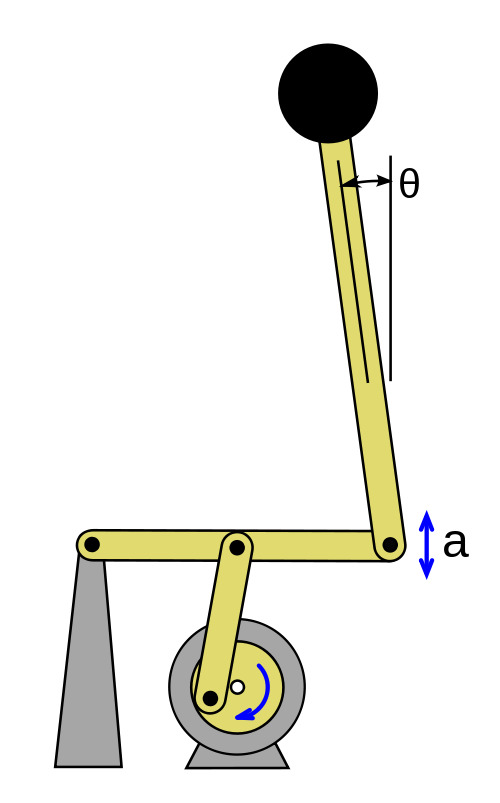
\includegraphics{figures/kapitza.png}}
\caption{Kapitza's pendulum (source: Wikipedia). \label{fig:kapitza}}
\end{center}
\end{figure}


Let $\ell$ denote the length of the rod of the pendulum. We assume the base is moving along the vertical axis as a function $u(t)$ of time (which plays the role of the ``control function'' in this problem), and denote by $x$ the angle the pendulum forms with the \emph{upward-pointing vertical}, so that $x=0$ (rather than $x=\pi$ with the more commonly used angular coordinate) represents the unstable equilibrium point of the inverted pendulum. The position of the swinging mass is $\mathbf{r}=(\ell\sin x, \ell \cos x + u(t))$. We can now write the kinetic energy, potential energy and the Lagrangian, as follows:
\eqst{
K &= \tfrac12 |\dot{\mathbf{r}}|^2 = \tfrac12\left( \ell^2 \dot{x}^2\cos^2 x + \ell^2 \dot{x}^2 \sin^2 x - 2 \ell \dot{u} \dot{x} \sin x + \dot{u}^2\right)
\\ &= \tfrac12 \ell^2 \dot{x}^2 + \tfrac12 \dot{u}^2 - \ell \dot{u} \dot{x} \sin x, \\
U &= g\ell \cos x + g u, \\
L &= \tfrac12 \ell^2 \dot{x}^2 + \tfrac12 \dot{u}^2 - \ell \dot{u} \dot{x} \sin x
-g\ell \cos x - g u. \\
}
Therefore we have
\eqst{
\pder{L}{x} &= -\ell \dot{u}\dot{x}\cos x + gl\sin x, 
\\
\pder{L}{\dot{x}} &= \ell^2 \dot{x} - \ell \dot{u}\sin x,
\\
\der{}{t}\left(\pder{L}{\dot{x}}\right) &= \ell^2 \ddot{x} - \ell \ddot{u}\sin x - \ell \dot{u}\dot{x} \cos x,
}
and the Euler-Lagrange equation for this Lagrangian is
\eqst{
\ddot{x} =\frac{g+\ddot{u}}{\ell} \sin x.
}
That is, the effect of the vertical driving acceleration $\ddot{u}(t)$ applied to the base point is to make the effective gravity felt by the pendulum change as a function of time. We shall now make some assumptions to simplify the analysis. First, we shall study the behavior in the vicinity of the rest point, so we can replace the equation with its linearized version
\eqst{
\ddot{x} = \frac{g+\ddot{u}}{\ell} x.
}
Next, we assume that $u(t)$ is a periodic function with period $2T$ and frequency $f = 1/2T$, and furthermore, we assume that its second derivative $\ddot{u}(t)$ takes only two values $\pm a$, changing its sign exactly every half-period $T$, so that the graph of $u$ over each half-period is a parabolic arc rather than the sinusoidal arc typically used for periodic motions (this can even be a realistic assumption depending on the way the driving mechanism operates in practice, but the main reason for assuming it is that it results in a simpler mathematical analysis); see Figure~\ref{fig:drivingforce}. With this assumption, the equation becomes
\eqst{
\ddot{x} = (\omega^2 \pm A^2) x,
}
with the notation $\omega=\sqrt{g/\ell}$, $A=\sqrt{a/\ell}$, and where ``$\pm$'' denotes the square wave function
\eqst{ \pm = \begin{cases} +1 & \textrm{if }\sin(2\pi f t)>0, \\ -1 & 
\textrm{if }\sin(2\pi f t)<0.
\end{cases}
}
We assume that $A>\omega$, i.e., the ``artificial gravity'' induced by the vibrations dominates the gravity of the more usual type. It can be easily checked that the amplitude $d$ of the oscillation is given by
\eqst{
d = \frac{T^2 a}{8}.
}

\begin{figure}
\begin{center}
\scalebox{0.8}{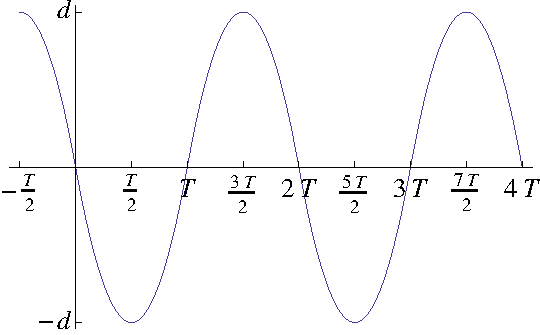
\includegraphics{figures/drivingforce.pdf}}
\caption{In our analysis, the driving function $u(t)$ for the height of the oscillating base is assumed to be periodic with period $2T$, and each half-period is a parabolic arc with second derivative $\pm a$ and amplitude $d$. \label{fig:drivingforce} }
\end{center}
\end{figure}


As a final notational step before we start the analysis, we do the usual trick of representing a second-order system as a planar first-order system:
\eqst{
\dot{x} &= y, \\
\dot{y} &= (\omega^2 \pm A^2) x.
}
Note that this is a linear, but time-dependent, system, so we can represent it in vector notation as
\eq{ \label{eq:kapitza-matrix}
\dot{\mathbf{x}} &= B_t \mathbf{x},
}
where $\mathbf{x}=(x,y)^\top$ and $B_t = \left( \begin{array}{cc} 0&1 \\ \omega^2\pm A^2 & 0 \end{array}\right)$. 

We are now in a position to study when (as a function of the parameters $a, T, \ell, g$) we can expect the system to be stable at $x=0$. 
The idea is to reduce the problem to understanding the stability of an autonomous discrete-time dynamical system which we can explicitly compute. For real numbers $t_0<t_1$, define a map $\psi_{t_0,t_1}:\R^2\to\R^2$, analogous to the phase flow map $\varphi_t$ we studied for autonomous systems, as follows:
\eqst{
\psi_{t_0,t_1}(\mathbf{x}_0) = &\ \mathbf{x}(t_1)\textrm{ where $\mathbf{x}(t)_{t\ge t_1}$ is the solution of the system \eqref{eq:kapitza-matrix}}\\ & \textrm{with initial condition $\mathbf{x}(t_0)=\mathbf{x}_0$}.
}
That is, $\psi_{t_0,t_1}$ evolves a point forward in time from time $t_0$ to time $t_1$. (In the case of an autonomous system, we could write this as $\varphi_{t_1-t_0}(\mathbf{x}_0)$ since it would depend only on the duration of the evolution rather than the specific starting and ending times.) The evolution maps $\psi_{t_0,t_1}$ have several important properties. First, they are linear, since the system \eqref{eq:kapitza-matrix} is linear. Second, they satisfy the composition property
\eqst{
\psi_{t_0,t_2}(\mathbf{x}_0) = \psi_{t_1,t_2}( \psi_{t_0,t_1}(\mathbf{x}_0)) \ \ (t_0<t_1<t_2),
}
or equivalently
\eq{ \label{eq:composition-prop}
\psi_{t_0,t_2}(\mathbf{x}_0) = \psi_{t_1,t_2}\circ \psi_{t_0,t_1}\ \ (t_0<t_1<t_2),
}
since evolving a solution from time $t_0$ to $t_2$ can be done by evolving it up to time $t_1$ and then evolving the resulting point from $t_1$ to $t_2$. Third, because the matrix function $t\mapsto B_t$ in the equation \eqref{eq:kapitza-matrix} is periodic with period $2T$, we have
\eqst{
\psi_{t_0+2T,t_1+2T}(\mathbf{x}_0) = \psi_{t_0,t_1}(\mathbf{x}_0).
}
By the composition property \eqref{eq:composition-prop}, we can now express the solution $\mathbf{x}(t)$ with an initial condition $\mathbf{x}(0)=\mathbf{x}_0$ at time $0$ as the result of a sequence of evolution steps along small time intervals of length $T$. More precisely, if $n$ is an integer such that $2nT \le t < 2(n+1)T$, then we have
\eq{
\begin{split}
\mathbf{x}(t) &= \psi_{0,t}(\mathbf{x}_0)
\\ &=
\psi_{T,t} \circ \psi_{0,T}(\mathbf{x}_0)
\\ &=
\psi_{2T,t} \circ \psi_{T,2T}\circ \psi_{0,T}(\mathbf{x}_0) =  \ldots 
\\ &= 
\psi_{2nT, t} \circ \psi_{(2n-1)T,2nT} \circ \ldots
\circ \psi_{2T,3T} \circ \psi_{T,2T}\circ \psi_{0,T}(\mathbf{x}_0)
\\ &=
\psi_{2nT, t} \circ S_- \circ S_+ \circ S_- \circ S_+ \circ \ldots \circ S_- \circ S_+ (\mathbf{x}_0)
\\ &=
\psi_{0, t-2nT} \circ (S_- \circ S_+)^n (\mathbf{x}_0) = \psi_{0, t-2nT} \circ P^n (\mathbf{x}_0),
\end{split}
\label{eq:kapitza-phase-flow}
}
where we denote
\eqst{
S_+ = \psi_{0,T}, \ \ \ S_- = \psi_{T,2T}, \ \ \ P= S_- \circ S_+ = \psi_{0,2T}.
}
The analysis will now revolve around an explicit computation of the $2\times 2$ matrices associated with the linear maps $S_\pm$ and their composition $P$, the \emph{period evolution map}. A key observation is the following:

\begin{lem}
If $|\operatorname{tr}(P)|<2$ then the system \eqref{eq:kapitza-matrix} has a stable rest point at $\mathbf{x}=\mathbf{0}$.
\end{lem}

\begin{proof}
$P$ is a $2\times 2$ matrix of real numbers with determinant $\det(P)=\det(S_-)\det(S_+)=1$ (this fact also follows from Liouville's theorem). Its eigenvalues $\lambda_1, \lambda_2$ are the roots of a quadratic polynomial with real coefficients, and satisfy 
\eqst{
\lambda_1 \lambda_2 &= \det(P)=1, \\ 
\lambda_1 + \lambda_2 &= \operatorname{tr}(P).
}
If both eigenvalues are real then the fact that $\lambda_2=1/\lambda_1$ implies that
\eqst{
|\lambda_1 + \lambda_2| = \left|\lambda_1 + \frac{1}{\lambda_1}\right| \ge 2,
}
in contradiction to the assumption that $|\operatorname{tr}(P)|<2$. The only other possibility is that $\lambda_1$ and $\lambda_2$ are conjugate complex numbers, which must lie on the unit circle, since $\lambda_1\lambda_2 = \lambda_1 \overline{\lambda_1}= |\lambda_1|^2 = 1$. This implies that for some constant $C>0$, we have
\eqst{
|P^n \mathbf{x}| \le C |\mathbf{x}|
}
for all $n\ge1$ and $\mathbf{x}\in \R^2$, since $\lambda_1=e^{i\theta}$ for some real $\theta$, and from linear algebra we know that by representing such a matrix in an appropriate basis one can bring it to the form of a rotation matrix $\left(\begin{array}{cc} \cos \theta & -\sin\theta \\ \sin\theta & \cos\theta\end{array} \right)$. In other words, this shows that the \emph{discrete-time} dynamical system defined by the matrix $P$ has a (neutrally) stable rest point at $\mathbf{x}=\mathbf{0}$.

Finally, observe that the family of matrices $(\psi_{0,s})_{0\le s\le 2T}$ is the image of a compact interval $[0,2T]$ under a continuous map $s\mapsto \psi_{0,s}$, and therefore this set of matrices is compact, and hence bounded in norm, in the space of $2\times 2$ matrices. Therefore there is some constant $D>0$ such that \eqst{
\max_{0\le s\le 2T} |\psi_{0,s}(\mathbf{y}) | \le D |\mathbf{y}|
}
for any $\mathbf{y}\in\R^2$. Combining this with the previous comment and with \eqref{eq:kapitza-phase-flow}, we get that
\eqst{
|\psi_{0,t} (\mathbf{x_0})| \le CD |\mathbf{x_0}|
}
for all $t\ge 0$, which shows that $\mathbf{x}=\mathbf{0}$ is a neutrally stable rest point of the system \eqref{eq:kapitza-matrix}.
\end{proof}

To compute $S_-$ and $S_+$, observe that they are both obtained by evolution of the system along time intervals for which the matrix $B_t$ is constant; for such intervals the system \eqref{eq:kapitza-matrix} behaves like an autonomous system, and can be solved explicitly using matrix exponentials.

\begin{lem} The matrices $S_\pm$ are given by
\eq{
S_+ &= \left(\begin{array}{cc}
\cosh\left(kT\right) & \frac{1}{k}\sinh\left(kT\right) 
\\[5pt] 
k\sinh\left(kT\right) & \cosh\left(kT\right)
\end{array}\right),
\\[3pt]
S_- &= \left(\begin{array}{cc}
\cos\left(jT\right) & \frac{1}{j}\sin\left(jT\right) 
\\[5pt] 
-j\sin\left(jT\right) & \cos\left(jT\right)
\end{array}\right),
\label{eq:kapitza-mat-exp}
}
where $k=\sqrt{A^2+\omega^2}=\sqrt{(a+g)/\ell}, j=\sqrt{A^2-\omega^2}=\sqrt{(a-g)/\ell}$.
\end{lem}

\begin{proof}
By the comment above, we have
\eqst{
S_+ &= \exp\left(T \left(\begin{array}{cc} 0 & 1 \\ k^2 & 0
\end{array} \right) \right) = \exp(M_+), \\
S_- &= \exp\left(T \left(\begin{array}{cc} 0 & 1 \\ -j^2 & 0
\end{array} \right) \right) = \exp(M_-),
}
where we denote $ M_+ = \left(\begin{array}{cc} 0 & T \\ k^2T & 0
\end{array}\right)$,
$ M_- = \left(\begin{array}{cc} 0 & T \\ -j^2 T & 0
\end{array}\right)$. Note that $M_\pm$ satisfy
\eqst{
M_+^2 = k^2 T^2 I, \ \ \ 
M_-^2 = -j^2 T^2 I.
}
As a result, it is easy to evaluate the matrix exponentials $\exp(M_\pm)$ by directly summing the power series $\sum_{n=0}^\infty \frac{1}{n!}M_{\pm}^n$ (since the even powers are scalar multiples of $I$ and the odd powers are scalar multiples of $M_\pm$) to obtain the expressions in \eqref{eq:kapitza-mat-exp}. The computation is left as an exercise.
\end{proof}

\beginexer Perform the power series summation outlined above to verify the formulas \eqref{eq:kapitza-mat-exp}.

\bigskip
The final step consists of studying $\operatorname{tr}(P)=\operatorname{tr}(S_- S_+)$ to show that for an appropriate choice of parameters, stability can be achieved. Denote
$\sigma = \sigma(a, g, \ell, T) = \operatorname{tr}(P)$.
By the formulas \eqref{eq:kapitza-mat-exp}, we have
\eqst{
\sigma &= 
2\cos\left(jT\right)\cosh\left(kT\right)
+ \left(\frac{k}{j}-\frac{j}{k}\right)
\sin\left(jT\right)\sinh\left(kT\right)
\\ &=
2\cos\left(T\sqrt{\frac{a-g}{\ell}}\right)
\cosh\left(T\sqrt{\frac{a+g}{\ell}}\right)
\\ & \qquad +
\left(\sqrt{\frac{a+g}{a-g}}-\sqrt{\frac{a-g}{a+g}}
\right)
\sin\left(T\sqrt{\frac{a-g}{\ell}}\right)
\sinh\left(T\sqrt{\frac{a+g}{\ell}}\right).
}
We can now prove:

\begin{thm}
There are values of the parameters $a, g, \ell, T$ for which Kapitza's pendulum is stable.
\end{thm}

\begin{proof} Using the metric system of units,
take $g=9.8\,\frac{\textrm{m}}{\textrm{sec}^2}$ (the Earth's gravitational constant),
$\ell = 20\, \textrm{cm}$, $d=1\,\textrm{cm}$, $f=40\,\textrm{sec}^{-1}$. With these values we 
have $T=\frac{1}{80}\,\textrm{sec}$, $a=512\,\frac{\textrm{m}}{\textrm{sec}^2}$.
For these parameters the computer returns the value
\eqst{
\sigma(a, g, \ell, T) = 1.97728\ldots,
}
so in particular $|\sigma|<2$ and the pendulum is stable.
\end{proof}

It is possible to get a better understanding of the subset of the parameter space for which the motion is stable, at least for oscillations with small amplitude and high frequency, that explains why the ``lucky'' numbers above work to produce a stable value $|\sigma|<2$. This can be done by introducing two dimensionless parameters $w,z$, defined by
\eqst{
w^2 &= \frac{g}{a}\ \ \  \textrm{(the ratio of ``natural'' to ``artificial'' gravity)}, \\
z^2 &= \frac{d}{\ell}\ \ \  \textrm{(the ratio of the oscillation amplitude to the pendulum length)},
}
and to consider a limit in which both variables $w,z$ tend simultaneously to $0$ (with the variable $T$ changing accordingly).

\beginexercise{Asymptotic stability regime of Kapitza's pendulum} Represent $\sigma$ as a function of the variables $w, z$, then expand $\sigma$ in a Taylor series in $w,z$, including all terms up to and including order $4$ (i.e., all monomials of the form $w^i z^j$ for $0\le i+j\le 4$). From this approximation, deduce that if $w,z\to 0$ in such a way that $w<cz$ where $c$ is a constant satisfying $0<c<\sqrt{2/3}$, then for small enough values of $w,z$ the stable regime $|\sigma|<2$ is entered, i.e., the motion becomes stable.



\subsection{Alternating gradient focusing}

While the example discussed above is interesting mostly for its curiosity value, the mathematical idea underlying it has found a serious application as a method for focusing beams of charged particles in particle accelerators. The method, known as \emph{alternating gradient focusing} or \emph{strong focusing}, is an essential piece of technology used in all particle accelerator designs since the invention of the technique in the early 1950's. Roughly, the idea is as follows. In particle accelerators, beams of charged particles moving at close to the speed of light are directed along an approximately circular path by passing them through a sequence of powerful magnets. To focus the beams in order to achieve a high-quality beam suitable for performing useful experiments, the magnetic fields are carefully designed to create magnetic analogues of optical lenses. However, due to the way the physical law (called the Lorentz force) that governs how charged particles are influenced by magnetic fields works, it turns out that these magnetic lenses can only focus a beam along one axis: if the lens focuses the beam along the $x$-axis (where we imagine the beam to be moving in the $y$-direction), then it will \emph{defocus} the beam along the $z$-axis, and vice versa. The alternating gradient focusing technique is based on the observation that a series of magnetic lenses that focus the beam along alternating axes (an $x$-focusing lens, followed by a $z$-focusing lens, followed by an $x$-focusing lens, etc.) will achieve a net focusing effect along \emph{both} axes! Mathematically, the analysis showing the validity of the idea is virtually identical to the stability analysis we performed above for the inverted pendulum with an oscillating base\footnote{see equations (2.11), (2.12), (2.33) and (2.34) in the paper \emph{Theory of the alternating gradient synchrotron}, by E.~D.~Courant and H.~S.~Snyder (Annals of Physics \textbf{3} (1958), 1--48), available online at
\href{http://ab-abp-rlc.web.cern.ch/ab-abp-rlc/AP-literature/Courant-Snyder-1958.pdf}{\tiny \texttt{http://ab-abp-rlc.web.cern.ch/ab-abp-rlc/AP-literature/Courant-Snyder-1958.pdf}}}.

\subsection{Electromagnetic levitation} 

A famous practical demonstration of control theory is that of electromagnetic levitation. This is a method for causing a small magnetic object to hover in the air by causing an electromagnet (a coil that behaves like a magnet when an electric current is passed through it) positioned above the object to pull on it, balancing the magnetic attraction force against the force of gravity. There are several known ways to achieve stable levitation, a few of which use physical principles that are unrelated to control theory (for example, one of the most amusing demonstrations of levitation was in an experiment performed by a group of Dutch researchers in the year 2000 that used the physical effect of \emph{diamagnetism} to levitate a live frog). However, the easiest---and from our point of view, the most interesting---approach is to modulate the attractive magnetic field of the electromagnet using a feedback control scheme.

We will discuss the following simple model for a levitation device. The levitating object is idealized as a particle moving along a one-dimensional (vertical) axis, whose position $x(t)$ satisfies the equation
\eqst{
\ddot{x} = \begin{cases} -1 & \textrm{if the electromagnet is off}, \\
1 & \textrm{if the electromagnet is on.}
\end{cases}
}
The idea is that when the electromagnet is turned off, the particle experiences a downward acceleration due to the effect of gravity, and when the electromagnet is switched on, the attractive magnetic force causes an upward acceleration that overcomes gravity and exactly negates it. For simplicity, we choose units such that the gravitational constant $g$ is equal to $1$, and assume that the acceleration when the electromagnet is switched on is exactly equal in magnitude (and opposite in its direction) to the gravitational acceleration. The control variable $u$ is a binary ``on/off'' variable that corresponds to the decision of when to activate the electromagnet (a control scheme based on a binary control variable is sometimes called a \emph{switching control}). Our goal is to design a feedback-based control rule
\eqst{ u = u(x, \dot{x}) }
(where we denote $u=\ddot{x}=\pm 1$ to correspond to the two states of the electromagnet) such that the system will have an asymptotically stable equilibrium point at $x=0$ to which all the orbits converge.

\subsubsection{A first attempt.} An obvious idea to try is to switch the electromagnet on when $x<0$ and off when $x>0$. That is, we try the control rule $u=-\operatorname{sgn}(x)$ (where $\operatorname{sgn}(x)=x/|x|$ is the signum function), leading to the equation of motion
\eq{  \label{eq:magnet-unstable}
\ddot{x} = \begin{cases} -1 & \textrm{if }x>0 \\ 1&\textrm{if }x<0\end{cases} \ = -\operatorname{sgn}(x).
}
This can be represented in the usual way as a planar system of first-order ODEs, namely
\eqst{\dot{x} = y, \quad \dot{y}= - \operatorname{sgn}(x).
}
It is not hard to see how to draw the phase portrait for this system. First, imagine that there is no electromagnet, which leads to the simpler system (describing simply the motion of a particle under a uniform gravitational force)
\eq{ \label{eq:gravity-system}
\dot{x} = y, \quad \dot{y}= -1.
}
The solutions of this equation take the form
\eqst{ x(t) = x_0 + y_0t -\tfrac12 t^2, \ \ y(t)=y_0-t, }
where $x_0$ is the initial position and $y_0$ is the initial velocity. 
We then have that $y=y_0-t$, and therefore
\eqst{
x = x_0 + y_0(y_0-y)-\tfrac12(y_0-y)^2 = (x_0+\tfrac12 y_0^2)-\tfrac12 y^2,
}
in other words, the solution curves of the system have the form $x=a-\tfrac12 y^2$ where $a$ is some arbitrary parameter. This leads to the phase portrait shown in Figure~\ref{fig:phasediag-gravity}.

\begin{figure}
\begin{center}
\scalebox{0.7}{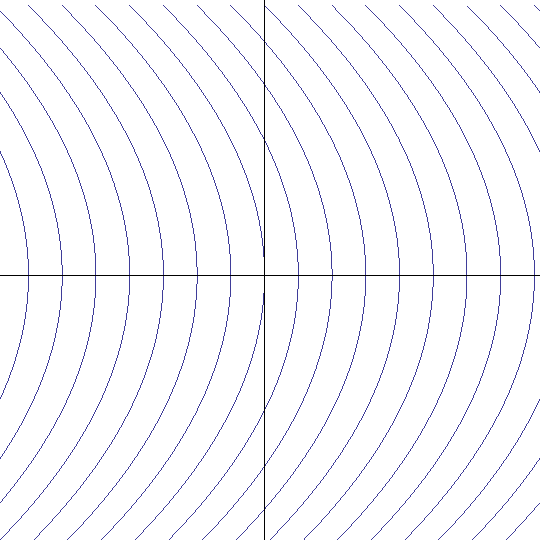
\includegraphics{figures/phasediag-gravity.pdf}}
\caption{The phase portrait for a particle falling under the influence of gravity. \label{fig:phasediag-gravity}}
\end{center}
\end{figure}

Next, the system \eqref{eq:magnet-unstable} consists of modifying the equation vector field by reflecting the flow curves for negative $x$ so that they mirror the lines for positive $x$. This leads to the phase portrait in Figure~\ref{fig:phasediag-magnet-unstable}. We see that the system indeed has a rest point at $(x,y)=(0,0)$. However, the rest point is a center, i.e., it is only neutrally stable (this is to be expected, since in fact this is an autonomous Hamiltonian system arising from a potential energy $U(x)=|x|$, and we know energy is conserved in such systems, leading to periodic oscillatory motions). So, a particle moving according to these equations of motion will indeed levitate, but will do so in a way that oscillates around the reference point $x=0$, and only under the unrealistic assumption that the physical system is indeed described to perfect precision by the equations \eqref{eq:magnet-unstable}. In practice, due to the finite speed of response of the switching control, any physical implementation of this control rule will be unstable.


\begin{figure}
\begin{center}
\scalebox{0.7}{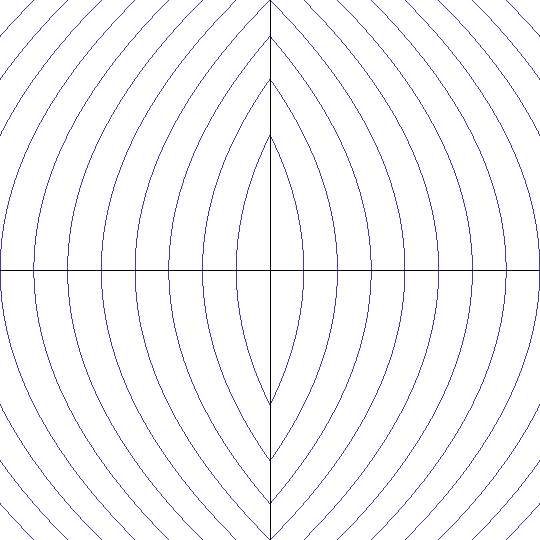
\includegraphics{figures/phasediag-magnet-unstable.pdf}}
\caption{The phase portrait for the equation of motion of a magnetically levitated object, using the ``naive'' approach. The rest point is only neutrally stable, and in practice this approach does not result in stable levitation. \label{fig:phasediag-magnet-unstable}}
\end{center}
\end{figure}


\subsubsection{Taking velocity into account}

It is apparent that to achieve stable levitation, a new idea is needed. Note that until now we only used information about the position of the particle. Why not use information about its velocity (the $y$ coordinate of the system's state $(x,\dot{x})$ when represented as a planar system) as well? Intuitively, this should help, since it's clear that the reason for oscillations developing in the previous scheme is that we are allowing the particle to overshoot the equilibrium point from either direction before toggling the state of the electromagnet; by looking at the velocity we could predict where the particle will be in a short time and do the toggling in advance in a way that will gradually reduce the size of the oscillations.

Formally, the idea described above leads to a feedback rule of the type
\eqst{ u = -\operatorname{sgn}(x+b\dot{x}), }
where $b>0$ is a small numerical constant. This leads to the modified system
\eqst{\dot{x} = y, \quad \dot{y}= - \operatorname{sgn}(x+b y).
}

To draw the phase portrait for the modified system, again one has to combine the curves from the simple gravity system \eqref{eq:gravity-system} with their mirror images, but the choice of which one to draw at a given point goes according to which side of the line $x+by=0$ the point is on. Finding the intersection points of the parabolas $x=a-\tfrac12 y^2$ and $x=a+\tfrac12y^2$ with the line $x+by=0$ leads to quadratic equations which are easily solved, so the phase portrait can be plotted fairly easily. The result is shown in Figure~\ref{fig:magnet-stable}.


\begin{figure}
\begin{center}
\scalebox{0.7}{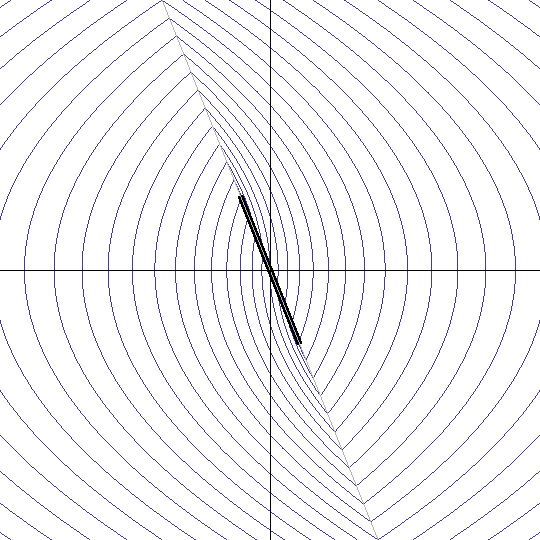
\includegraphics{figures/phasediag-magnet-stable.pdf}}
\caption{A feedback rule based on a linear combination of position and velocity leads to stable levitation. The final stage of the convergence to the equilibrium point is a non-smooth ``sliding motion'' along a ``chattering curve'', shown in black. \label{fig:magnet-stable}}
\end{center}
\end{figure}

A look at the phase portrait suggests that the idea is successful, and indeed results in stable levitation. It is not difficult to confirm this analytically. One interesting behavior that emerges upon closer examination of the properties of this system is that when $(x,y)$ crosses the switching line $x+by=0$, if the point is close enough to the origin then the equation of motion becomes ill-defined, since the vector field $(y,-\operatorname{sgn}(x+by))$ starts pointing back towards the switching line. In practice, due to time-delay effects in any physical implementation of the system, the particle will undergo a ``sliding motion'' in which it oscillates violently around both sides of the switching motion, all the while still sliding towards the origin. This phenomenon has been referred to as \emph{chattering}, since in physical implementations where the binary switching is done using an electrical relay, the high frequency switching makes a chattering noise. We can estimate the rate at which the particle will approach the origin during the sliding motion stage: since the sliding motion happens very near the line $x+by=0$ and we have the equation $\dot{x}=y$, the particle's position will approximately satisfy the ODE $\dot{x}=-x/b$, whose solution is given by
\eqst{
x(t) = c e^{-t/b}.
}
That is, the convergence to the origin in the final sliding stage is exponential, with a time constant of $1/b$.

\beginexer 
\begin{enumerate}
\item Show that the sliding motion for points along the line $x+by=0$ happens precisely for $|x|\le b^2$.
\item If we start the system at a point $(x_0,y_0)$ that lies on the switching line $x+by=0$, find a formula for the time it takes the point to flow into the sliding motion area connecting the points $(-b^2,b)$ and $(b^2,-b)$.)
\end{enumerate}

\subsubsection{Optimal switching control.} Although we have achieved our goal of designing a stable levitation control scheme, it is not necessary to stop here. A natural question is to ask for the \emph{optimal} control rule, namely the one that causes the particle to reach the stable equilibrium point in the shortest time, regardless of its initial conditions. Using ideas from the theory of nonlinear optimal control which are beyond the scope of this course, it is possible to prove that the optimal control rule is
\eqst{
u(x) = -\operatorname{sgn}\left(x+\tfrac12 \dot{x}|\dot{x}|\right).
}
This makes intuitive sense, since the idea behind this control rule is to toggle the electromagnet as soon as the state of the system reaches the curve $x=\tfrac12 y|y|$. The flow from that point on takes place along the parabola $x=\tfrac12 y^2$ (if $x>0$) or $x=-\tfrac12 y^2$ (if $x<0$) and leads directly to the origin with no further toggling of the controller's state required. The phase portrait of the system governed by this control rule is shown in Figure~\ref{fig:magnet-optimal}.

\begin{figure}
\begin{center}
\scalebox{0.7}{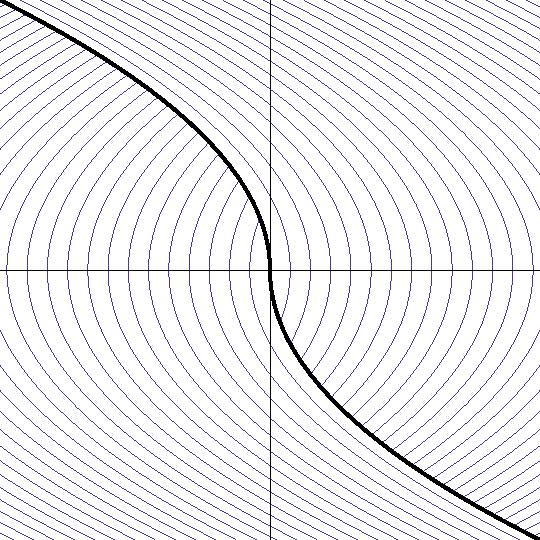
\includegraphics{figures/phasediag-magnet-optimal.pdf}}
\caption{Phase portrait for the optimal switching control. \label{fig:magnet-optimal}}
\end{center}
\end{figure}


\beginexercise{Optimal switching time} Find a formula for the time $\tau(x,\dot{x})$ it takes the particle to get to the origin when the optimal switching rule is used.
% *** note to self: the answer is:
%\eqst{
%T(x,y) = \begin{cases}
%y+2 \sqrt{x+\tfrac12 y^2} & \textrm{if }x>\tfrac12 y|y|, \\
%-y+2\sqrt{-x+\tfrac12 y^2} & \textrm{if }x\le \tfrac12 y|y|.
%\end{cases}
%}
% ***

\begin{figure}
\begin{center}
\scalebox{0.13}{\rotatebox{270}{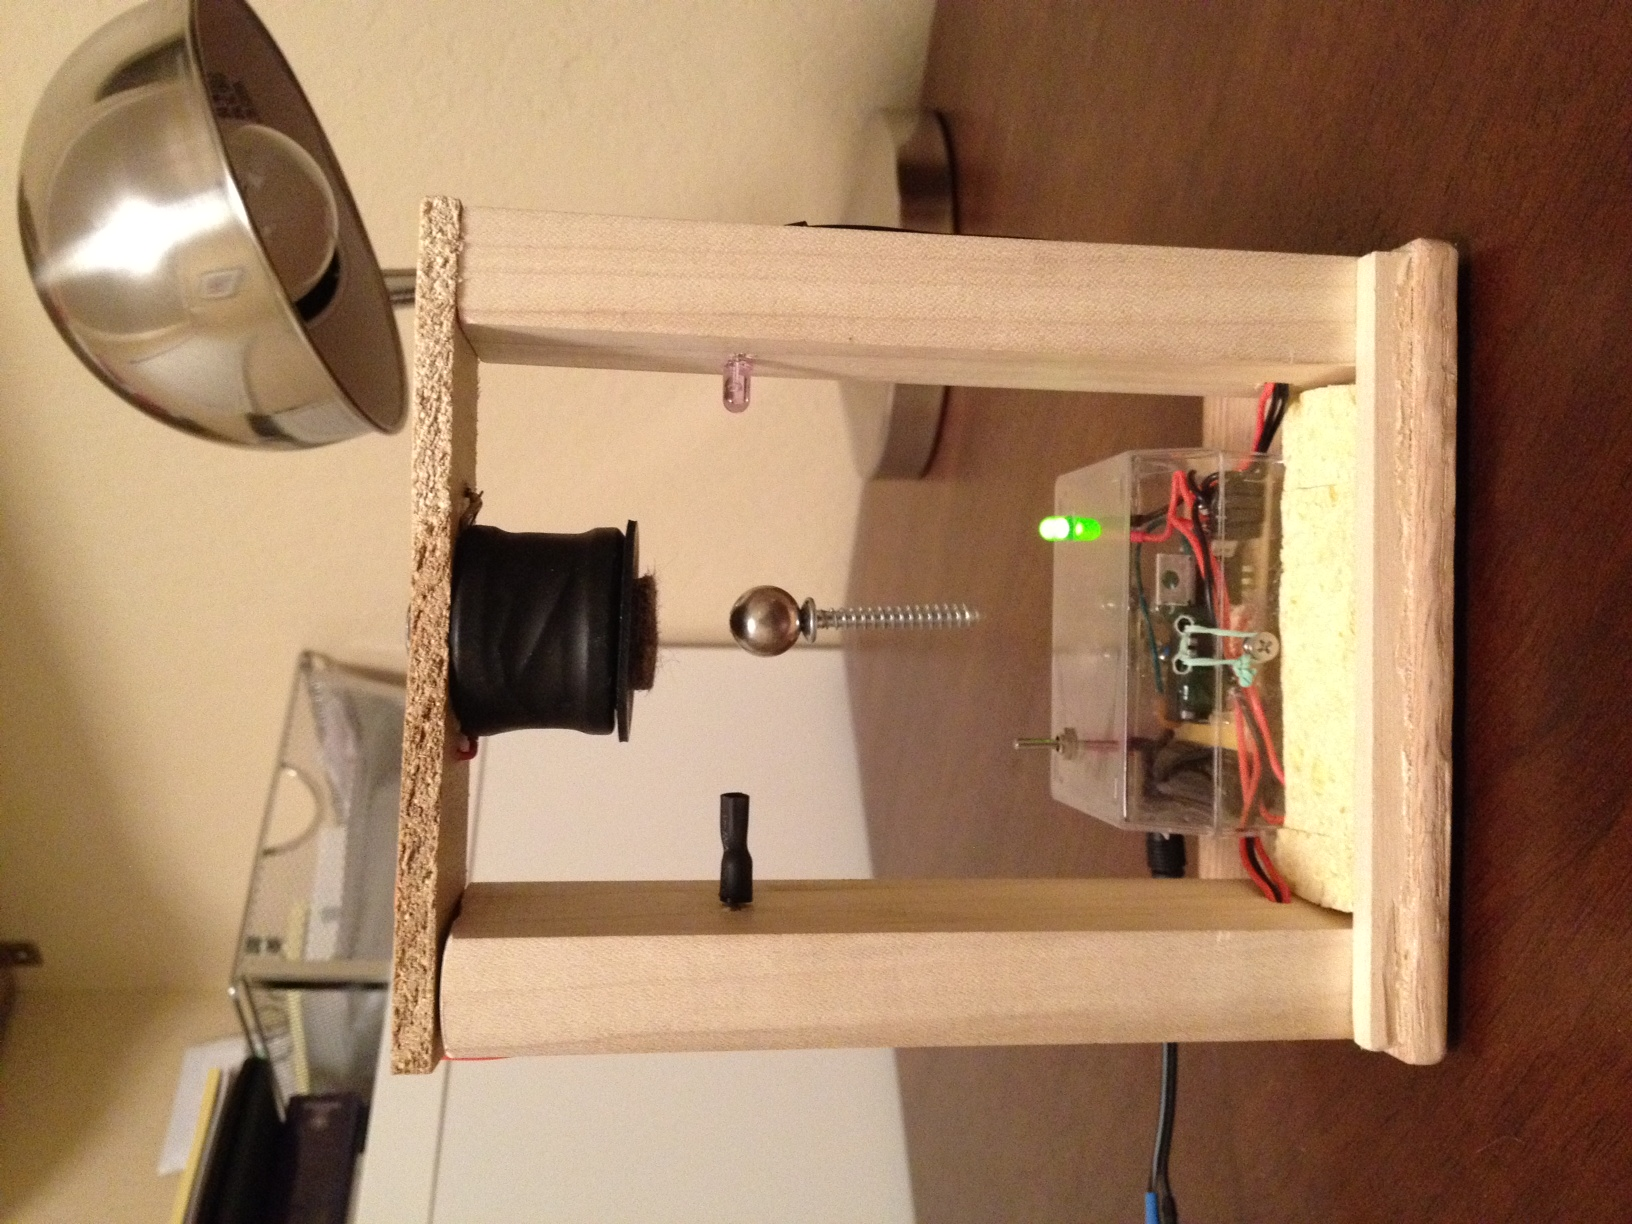
\includegraphics{figures/levitator1.JPG}}}
\caption{A homemade electromagnetic levitation device.}
\end{center}
\end{figure}


\subsection{Linear Quadratic Performance control}

In this section we consider control problems which take the general form
\eq{ \label{eq:lqp-linear}
\dot{\mathbf{x}} = A \mathbf{x} + B \mathbf{u},
}
where the state $\mathbf{x}$ of the dynamical system is an $n$-dimensional vector, the control variable $\mathbf{u}$ is an $m$-dimensional vector, and $A, B$ are linear operators (i.e., $A$ is an $n\times n$ matrix and $B$ is an $n\times m$ matrix). The goal of the control will be to bring the dynamical variable $\mathbf{x}$ to the origin. Moreover, we associate with any proposed solution a \emph{cost functional} that measures how effective it is. The cost functional will take the form
\eq{ \label{eq:lqp-quadratic}
J = \int_{t_1}^{t_2}
\left( \mathbf{x}^\top P \mathbf{x} + \mathbf{u}^\top Q \mathbf{u} \right)\, dt,
}
where $-\infty<t_1<t_2\le \infty$, $P$ is an $n\times n$ positive-definite matrix and $Q$ is an $m\times m$ positive-definite matrix. The idea is that we want to incentivize the controller to bring $\mathbf{x}$ to the origin as fast as possible by ``pushing'' on it as hard as possible; at the same time, in a typical situation the ``pushing'' also incurs a price since it uses resources  such as electricity, fuel, etc. The problem of optimal control is to find the feedback-based solution $\mathbf{u}=\mathbf{u}(\mathbf{x})$ that minimizes the overall cost functional, which finds a balance between the cost of resources and the desire to achieve good performance. It turns out that the solution has the form
\eq{ \label{eq:lqp-gain-mat}
\mathbf{u} = -K \mathbf{x},
}
where $K$ is a time-dependent linear operator which we will identify. Usually $K$ is expressed in the form $K(t_2-t)$, i.e., as a function of the ``time-to-go'' variable $T=t_2-t$. The most interesting case is that of an infinite time horizon: $t_2=\infty$; in this case we look for a stationary solution in which $K$ is a constant matrix, called the \emph{gain matrix}.

Note that the mapping that takes a pair $(\mathbf{u},\mathbf{a})$ where $\mathbf{u}$ is the control function and $\mathbf{a}$ is the initial condition $\mathbf{x}(t_1)=\mathbf{a}$ to the solution of \eqref{eq:lqp-linear} is linear, and the cost functional \eqref{eq:lqp-quadratic} is a quadratic expression in $\mathbf{x}$ and $\mathbf{u}$. Thus this type of problem is referred to as Linear Quadratic Performance (LQP) control. The main advantage of LQP control problems is that they have an explicit solution in terms of an ordinary differential equation, the Ricatti equation, which furthermore is easy to solve numerically.

\subsubsection{The one dimensional LQP control problem} Since the problem in this generality is somewhat complicated to analyze, to illustrate the main ideas we will focus on a simple one-dimensional settting in which $m=n=1$, the differential equation becomes
\eqst{
\dot{x} = ax+bu 
}
for some constants $a,b\in\mathbb{R}$, and the cost functional takes the form
\eqst{
I = \int_{t_1}^{t_2} (px^2+qu^2)\,dt
}
for some numbers $p,q>0$. Note that, for a given control rule, to compute $I$ all that one needs to know is the initial condition $x(t_1)$ and the duration $T=t_2-t_1$ over which the cost is integrated (that is, changing the left endpoint $t_1$ of the interval $[t_1,t_2]$ while keeping its length fixed will not change the cost functional). Let $I_*(w,T)$ denote the optimal control cost associated with an initial condition $x(t_1)=w$ and an interval $[t_1,t_2]$ of length $T$:
\eqst{
I_*(w,T) = \min_{\textrm{control rule $u$}} \int_{t_1}^{t_1+T} (p x^2+qu^2)\,dt
\ \qquad (x(t_1)=w).
}
In the derivation that follows, we assume that $t_2<\infty$ and that $I_*(w,T)$ is a smooth function of $w$ and $T$. Furthermore, it is not hard to see due to the quadratic nature of $I$ that the dependence of $I_*(w,T)$ on $w$ is also quadratic, i.e., we can write
\eqst{
I_*(w,T) = v(T) w^2
}
for some smooth function $v(T)$. The variable $T=t_2-t_1$ is nonnegative, and for $T=0$ we clearly have $v(0)=0$.

Now, let $\delta$ be a small positive number. We separate the interval $[t_1,t_2]$ into the subintervals $[t_1,t_1+\delta]$ and $[t_1+\delta,t_2]$. When optimal control is used for the entire interval $[t_1,t_2]$, in particular the control rule for each subinterval is also optimal. Thus, we have the equation
\eq{ \label{eq:lqp-subintervals}
I_*(w,T) = I_*(w,\delta) + I_*(z,T-\delta),
}
where $z=x(t_1+\delta)$ is the value obtained from the solution of the optimal control problem with initial condition $x(t_1)=w$ for the interval $[t_1,t_1+\delta]$. When $\delta$ is small, we have the following linear approximations in $\delta$:
\eq{ \label{eq:lqp-approx}
I_*(w,\delta) &= (p w^2 + q u_*^2)\delta + O(\delta^2), \\ 
z &= w + \dot{x}(0)\delta + O(\delta)^2 = w + (aw+b u_*)\delta + O(\delta^2),
}
where $u_*$ is the value of the control variable at time $t=t_1$ when optimal control is used with initial condition $x(t_1)=w$ over the interval $[t_1,t_2]$. Note that like $I_*$, $u_*$ depends only on $w$ and $T=t_2-t_1$. Furthermore, by dimensional considerations, the dependence of $u_*$ on $w$ is linear, so we may write
\eqst{
u_* = - k(T)w. 
}
The scalar quantity $k(T)$ is a gain factor, analogous to the operator $K$ mentioned above in connection with the LQP control problem in arbitrary dimension.

Now, continuing \eqref{eq:lqp-subintervals}, we may further expand all terms on the right-hand side as linear approximations in $\delta$:
\eqst{
I_*(w,T) &= I_*(w,\delta) + I_*(z,T-\delta)
\\ &= (p w^2 + q u_*^2)\delta \\ & \qquad +
I_*(w,T) + \pder{I_*}{w}(w,T)(z-w) + \pder{I_*}{T}(w,T)(-\delta) + O(\delta^2)
\\ &=
I_*(w,T) + \delta\left[
(p w^2+qu_*^2) + 2w v(T)(aw+b u_*) - v'(T) w^2
\right]
 \\ & \qquad + O(\delta^2).
}
In the limit when $\delta\downarrow 0$ we therefore get that
\eqst{
(p w^2+qu_*^2) + 2w v(T)(aw+b u_*) - v'(T) w^2 = 0,
}
or, substituting $-k(T)w$ for $u_*$, we have the equation
\eqst{
w^2\left(
p + q k^2 + 2av(T) -2 b k v(T) -v'(T)
\right) = 0,
}
where we write $k$ instead of $k(T)$. Since $w$ is arbitrary, we get the relation
\eq{ \label{eq:lqp-quadratic-poly}
p + q k^2 + 2av(T) -2 b k v(T) -v'(T) = 0.
}
We still don't know $k$ (or equivalently, $u_*$); but now, recalling that $u_*$ was defined from the value of the control variable \emph{under optimal control}, we see that the left-hand side of \eqref{eq:lqp-quadratic-poly}, which is a quadratic polynomial in $k$, must take its minimum at the correct value $k=k(T)$:
\eqst{
k &= \textrm{value of $s$ for which }\  qs^2-2b v(T) s + p-v'(T)\ \textrm{ is minimized}
\\ &= \frac{b v(T)}{q}.
}
(Recall that a quadratic polynomial $a_2s^2+a_1s+a_0$ has its extremum point when $s=-a_1/2a_2$, as can be seen by equating its derivative to~$0$).

Summarizing, we have found that the unknown gain function $k(T)$ is given by $k(T) = b v(T)/q$, where $v(T)$, heretofore also unknown, is the solution of the differential equation
\eq{ \label{eq:lqp-ricatti1}
v'(T) = p + 2 a v(T) - \frac{b^2}{q} v(T)^2
}
obtained by plugging the expression for $k(T)$ back into \eqref{eq:lqp-quadratic-poly}, with the initial condition $v(0)=0$. This is the \emph{Ricatti equation with constant coefficients}.

\subsubsection{The case of an infinite time horizon} The case $t_2=\infty$ can be approached by letting $T\to\infty$ in the equation above. The solution $v(T)$ of the Ricatti equation should converge to a stationary point satisfying $v'(T)=0$, so we get for this case that the limiting value $v_\infty$ of $v(T)$ must satisfy the quadratic equation
\eqst{ 
v_\infty^2 - \frac{2aq}{b^2} v_\infty - \frac{pq}{b^2} = 0, 
}
giving that
\eqst{
v_\infty = \frac{aq}{b^2}\left( 1 \pm \sqrt{1+\frac{pb^2}{qa^2}}\right).
}
Since we know that $v_\infty\ge 0$ and $p,q>0$, it can be checked that the correct choice of sign is:
\eqst{
v_\infty = \begin{cases}
\frac{aq}{b^2}\left( 1 - \sqrt{1+\frac{pb^2}{qa^2}}\right)
&
\textrm{if }a<0,  \\
\frac{aq}{b^2}\left( 1 + \sqrt{1+\frac{pb^2}{qa^2}}\right)
&
\textrm{if }a>0.
\end{cases}
}
The optimal control gain $k=k_\infty$ is then given as before by $k_\infty = b v_\infty/q$.
Note that the case $a<0$ corresponds to a situation in which the object is stable even in the absence of a control force, i.e., if we take $u=0$.

\subsubsection{Generalization to arbitrary dimension}

By repeating the above analysis in a careful manner for the general LQP problem in arbitrary dimension discussed at the beginning of this section, one can derive the solution for that general case. For the LQP problem with a finite horizon, the gain matrix $K(T)$ from \eqref{eq:lqp-gain-mat} is expressed as a matrix product
\eqst{
K(T) = Q^{-1}B^\top V(T),
}
where $V(T)$ is a matrix related to the optimal cost function $J_*(\mathbf{w},T)$ (defined analogously to $I_*(w,T)$) by
\eqst{
J_*(\mathbf{w},T) = \mathbf{w}^\top V(T)\mathbf{w}.
}
Furthermore, $V$ satisfies the matrix differential equation (also referred to as the Ricatti equation)
\eqst{
\der{V}{t} = P + A^\top V(T) + V(T) A - V(T) B Q^{-1} B^\top V(T)
}
with boundary condition $V(0) = 0$ (the zero matrix). For an infinite time horizon, we again look for stationary solutions, which leads to the \emph{algebraic Ricatti equation}
\eqst{
P + A^\top V + V A - V B Q^{-1} B^\top V = 0,
}
which is a system of quadratic equations in the entries of $V$.
The (constant) gain matrix $K$ is again given by
\eqst{
K = Q^{-1}B^\top V.
}
While these equations may seem intimidating at first sight, they are easy to solve numerically on a computer. Symbolic math software applications such as \texttt{Mathematica} even contain specialized packages for control theory that make the process of deriving optimal LQP control rules highly automated and quite simple in practice, as the next example demonstrates.

\beginexample{The inverted pendulum with cart: \textnormal{LQP} optimal control with \textnormal{\texttt{Mathematica}}}\footnote{This example is based on a blog post written by Andrew Moylan on the website of Wolfram Research (maker of the \texttt{Mathematica} software); see the link: \\
\href{http://blog.wolfram.com/2011/01/19/stabilized-inverted-pendulum/}{\texttt{http://blog.wolfram.com/2011/01/19/stabilized-inverted-pendulum/}}\,.}
The controlled inverted pendulum with cart is a dynamical system with 2 degrees of freedom $\theta=\theta(t)$ (representing the angle of the pendulum relative to the positive $x$-axis) and $x=x(t)$ (representing the displacement of the cart along the $x$-axis), satisfying the equations of motion
\eqst{
4\ddot{x} &=  \ddot{\theta}\sin \theta + \dot{\theta}^2 \cos \theta + 2 u, \\
0 &= \ddot{\theta}+2\cos \theta - 2\ddot{x} \sin\theta,
}
where $u$ is the control variable representing a control force being applied to the cart---see Figure~\ref{fig:invertedpendulum-cart}. 

\begin{figure}
\begin{center}
\scalebox{0.7}{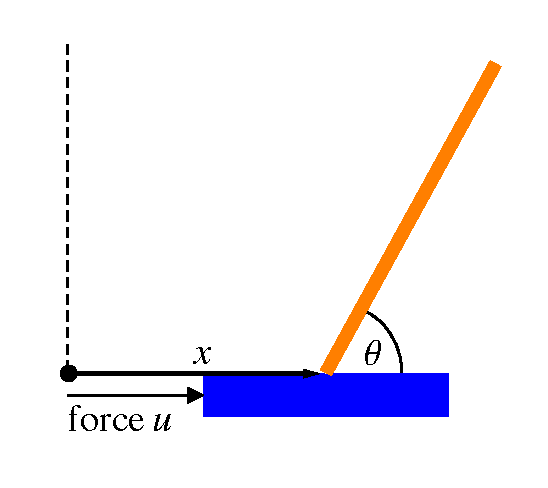
\includegraphics{figures/invertedpendulum-cart.pdf}}
\caption{The inverted pendulum and cart. \label{fig:invertedpendulum-cart}}
\end{center}
\end{figure}

The system can be thought of in the usual way as a system of 4 coupled first-order ODEs in the variables $\theta, \dot{\theta}, x, \dot{x}$. The goal of the control problem is to bring the system to a stable equilibrium at $(x,\dot{x},\theta,\dot{\theta}) = (0,0,\pi/2,0)$. 
In \texttt{Mathematica}, we type the following commands:

\vspace{-10.0pt}
\begin{quote}
\eqst{
\scriptsize{\textcolor{blue}{\text{In[1]=}}}\quad & \text{eqns}=\left\{2 u[t]+\text{Cos}[\theta [t]] \theta '[t]^2+\text{Sin}[\theta [t]] \theta ''[t]==4 x''[t], \right.\\ & \qquad\qquad \qquad  \qquad \left. 2 \text{Cos}[\theta [t]]-2 \text{Sin}[\theta [t]] x''[t]+\theta ''[t]==0\right\};
\\
\scriptsize{\textcolor{blue}{\text{In[2]=}}}\quad &\text{model}=\text{StateSpaceModel}\Big[\text{eqns}, \\ & \qquad\qquad \left\{\{x[t],0\},\{x'[t],0\},\left\{\theta [t],\frac{\pi }{2}\right\},\{\theta '[t],0\}\right\},u[t],\{\},t\Big]
\\
\scriptsize{\textcolor{blue}{\text{Out[2]=}}}\quad &
\left(
\begin{array}{cccc|c}
 0 & 1 & 0 & 0 & 0 \\
 0 & 0 & 1 & 0 & 1 \\
 0 & 0 & 0 & 1 & 0 \\
 0 & 0 & 4 & 0 & 2 \\
\end{array}
\right)_{}^{\mathcal{S}}
}
\end{quote}
The second command causes \texttt{Mathematica} to linearize the equations of motion around the desired rest point. The output is an augmented matrix of the form $\left( A\,|\,B\right)$ where $A, B$ are the two matrices in the resulting linearized equation \eqref{eq:lqp-linear}. This brings the problem to the familiar setup of LQP optimal control which we discussed above. We now type:
\eqst{
\scriptsize{\textcolor{blue}{\text{In[3]=}}}\quad &
\text{gains}=\text{LQRegulatorGains}[\text{N}[\text{model}],
\\ & \qquad\qquad
\{\text{DiagonalMatrix}[\{1,10,10,100\}],\{\{1\}\}\}]\text{//}\text{First}
\\
\scriptsize{\textcolor{blue}{\text{Out[3]=}}}\quad &
\{-1.,-5.97415,14.8452,13.7966\}
}
This asks \texttt{Mathematica} to compute the gain matrix $K$ (in this case a vector with 4 coordinates) associated with the cost functional 
\eqref{eq:lqp-quadratic} (in the case $t_2=\infty$ of an infinite time horizon), where the quadratic forms $P, Q$ are defined by
\eqst{
P = \left(\begin{array}{cccc}
1&0&0&0\\0&10&0&0\\0&0&100&0\\0&0&0&1000
\end{array}\right),
\qquad
Q = (1).
}
Using the gain matrix computed by \texttt{Mathematica}, we see that the solution to the optimal control problem we defined is given by the feedback rule
\eqst{
u = - x -5.97415\, \dot{x} + 14.8452\, \theta + 13.7966\, \dot{\theta}.
}


\vspace{10.0pt}
\begin{center}
\textbf{End of Part 3}
\end{center}

\newpage

\section*{Bibliographic notes}

Here are the main sources I used during the preparation of these lecture notes. I had a lot of fun consulting these books, but had to leave out many beautiful topics. The interested reader is encouraged to continue his or her journey into the world of ODEs by looking into these more detailed sources. I especially recommend the books by Arnold, Banks and anything written by Richard Feynman (including his hilarious memoir \textit{Surely You're Joking, Mr. Feynman}).

\bigskip

\noindent \textbf{Sources for Part 1}
\begin{enumerate}
\item V.~I.~Arnold, Mathematical Methods of Classical Mechanics, 2nd Ed. Springer, 1988.
\item R.~B.~Banks, Towing Icebergs, Falling Dominoes, and Other Adventures in Applied Mathematics. Princeton University Press, 1998.
\item R.~Grimshaw, Nonlinear Ordinary Differential Equations. Blackwell Scientific Publications, 1990.
\item J.~K.~Hunter, Lecture Notes on Applied Mathematics, available online at
\\
\href{http://www.math.ucdavis.edu/~hunter/m280_09/applied_math.html}{\texttt{http://www.math.ucdavis.edu/}\textasciitilde\texttt{hunter/m280\_09/applied\_math.html}}
\item L.~A.~Pars, An Introduction to the Calculus of Variations. Heinemann Educational Books, 1962 (reprinted by Dover Publications, 2010).
\suspend{enumerate}

\noindent \textbf{Sources for Part 2}
\resume{enumerate}
\item D.~Romik, Lecture Notes for Math 235B: Probability Theory, available online at
\\ 
\href{http://www.math.ucdavis.edu/~romik/teaching/mat235-2011-2012/#235b}{\texttt{http://www.math.ucdavis.edu/}\textasciitilde\texttt{romik/teaching/mat235/\#235b}}
\item S.~H.~Strogatz, Nonlinear Dynamics and Chaos. Westview Press, 1994.
\suspend{enumerate}

\noindent \textbf{Sources for Part 3}
\resume{enumerate}
\item Chapter 5 of Arnold's book listed above.
\item R.~P.~Feynman, R.~B.~Leighton, M.~Sands, The Feynman Lectures on Physics, Vol. II. Basic Books, 1964. (Chapter 29 has a discussion of alternating-gradient focusing and the inverted pendulum with an oscillating base.)
\item O.~L.~R.~Jacobs, Introduction to Control Theory. Oxford Science Publications, 1993.
\end{enumerate}

\end{document}

\newpage

\newpage

\eqst{
\dot{\mathbf{x}} = \mathbf{A} \mathbf{x} + \mathbf{B} \mathbf{u}
}

\eqst{
\mathbf{u} = -\mathbf{K} \mathbf{x}
}

\eqst{
J = \int_{t_1}^{t_2}
\left( \mathbf{x}^\top \mathbf{P} \mathbf{x} + \mathbf{u}^\top \mathbf{Q} \mathbf{u} \right)\, dt.
}

\eqst{\dot{x} = ax+bu }
\eqst{I = \int_{t_1}^{t_2} (px^2+qu^2)\,dt}



\newpage
\ 

\newpage

\subsection{Linear systems}

\subsubsection{Matrix exponentials}

\subsubsection{Stability analysis}

\subsubsection{Linearization of nonlinear systems}

\subsection{Open-loop control}

\subsubsection{Stabilizing an inverted pendulum with vertical oscillations}

\subsubsection{Alternating gradient focusing}

\subsection{Control with feedback}

\subsection{PID control}

\subsection{Linear quadratic regulator}

\subsection{Low pass and high pass filters}

\subsection{Examples}

\subsubsection{Inverted pendulum}

\subsubsection{Electromagnetic levitation} single threshold, two thresholds

\subsubsection{Bicycle}





\section{Miscellaneous topics}

\subsection{ODE proof of the fundamental theorem of algebra}




\subsection{Random ideas}
Particle in free space, particle in uniform gravitational field, harmonic oscillator, pendulum, rotating pendulum, double pendulum, spinning top, levitron

(Material for exercises: physical analogs of a pendulum: Josephson junction and elastic rods; analytic solution of pendulum; application to falling domino waves)




\end{document}